\documentclass[12pt, a4paper]{report}

% --- Packages ---
\usepackage[margin=2.5cm]{geometry}
\usepackage{setspace}
\usepackage{graphicx}
\usepackage{float}
\usepackage{booktabs}
\usepackage{hyperref}
\usepackage{listings}
\usepackage{amsmath}
\usepackage{cite}
\usepackage{microtype}
\usepackage{xcolor}
\usepackage{caption}
\usepackage{subcaption}
\usepackage{multirow}
\usepackage{tikz}
\usepackage{algorithm}
\usepackage{algpseudocode}
\usetikzlibrary{arrows.meta, positioning, fit, backgrounds}

\onehalfspacing

% --- Code listing style ---
\lstset{
    basicstyle=\ttfamily\small,
    breaklines=true,
    frame=single,
    numbers=left,
    numberstyle=\tiny,
    tabsize=4
}

% --- Prettier C listing style (used for short code snippets) ---
\definecolor{codebg}{RGB}{248,248,248}
\definecolor{codeframe}{RGB}{210,210,210}
\definecolor{codekw}{RGB}{0,86,156}
\definecolor{codecomment}{RGB}{106,115,125}
\definecolor{codestring}{RGB}{163,21,21}
\definecolor{codenum}{RGB}{150,150,150}

\lstdefinestyle{csnippet}{
    language=C,
    basicstyle=\ttfamily\footnotesize,
    keywordstyle=\color{codekw}\bfseries,
    commentstyle=\color{codecomment}\itshape,
    stringstyle=\color{codestring},
    numberstyle=\tiny\color{codenum},
    backgroundcolor=\color{codebg},
    rulecolor=\color{codeframe},
    frame=single,
    framerule=0.4pt,
    rulesep=2pt,
    numbers=none,
    xleftmargin=10pt,
    xrightmargin=4pt,
    aboveskip=10pt,
    belowskip=10pt,
    showstringspaces=false,
    breaklines=true,
    tabsize=4,
    captionpos=b,
    columns=fullflexible,
    keepspaces=true,
    morekeywords={uint8_t,uint32_t,int64_t,size_t}
}

% ============================================================
\begin{document}
% ============================================================

% ---- Title Page --------------------------------------------
\begin{titlepage}
    \centering
    \vspace*{2cm}
    {\Large University College London \par}
    {\large Department of Computer Science \par}
    \vspace{2cm}
    {\LARGE\bfseries Enabling Modularity in IoT: Running WebAssembly Containerized
Workloads on Microcontrollers \par}
    \vspace{1cm}
    {\large Ahmed Ansari \par}
    \vspace{0.5cm}
    {\large MEng Computer Science \par}
    \vspace{0.5cm}
    {\large Supervisor: Stefano Vissicchio \par}
    \vspace{0.5cm}
\end{titlepage}
 


% ---- Abstract ----------------------------------------------
\chapter*{Abstract}

Microcontroller firmware is usually deployed as a monolithic, architecture-specific image, which limits update granularity and fault isolation. WebAssembly offers a portable and sandboxed execution model, but its practicality on resource-constrained control devices remains uncertain.

This project evaluates the WebAssembly Micro Runtime (WAMR) on an ESP32 using a two-board Hardware-in-the-Loop thermal testbed. The same bang-bang, PID, and step-response workloads are implemented in native C and in WebAssembly, then executed using the WAMR interpreter and WAMR ahead-of-time (AOT) mode. This allows the runtime cost to be measured from individual host calls through to full system behaviour, including fault recovery, update cost, inter-container communication, and multi-container scaling.

Running the same workloads across native C and WAMR produced equivalent control behaviour at a 100~ms period, with total wall-clock overhead below 0.2\%. The finer-grained measurements showed that overhead still depended strongly on execution mode. Interpreter mode added about 59~\textmu{}s to temperature reads and 113~\textmu{}s to heater writes, while AOT reduced these penalties to about 23--25~\textmu{}s. WAMR also used an additional 76--86~KB of heap memory. The runtime contained injected faults without rebooting the device and reduced logic-only update time from 20.15~s to 7.60~s. In the scaling experiments, interpreter mode failed at seven active containers due to CPU and scheduler pressure, while AOT remained stable up to eleven containers and then failed due to memory exhaustion. Overall, WAMR AOT was the most practical mode for this workload.

\chapter*{Acknowledgements}
\begingroup
\setlength{\parindent}{0pt}
\setlength{\parskip}{1em}

I would like to express my sincere gratitude to my supervisor, Professor Stefano Vissicchio, for his invaluable guidance, support, and kindness.

This work is dedicated to my best friend, Muhammad Abdullah, who departed this world too soon and is dearly missed. I know that part of him lives on in the lives he touched, and in the boundless love and happiness he shared with those closest to him.

I also want to thank my friends, who gave me an endless stream of precious memories and supported me through difficult times. I hope we have many more opportunities for banter, adventure, and growth together.

Lastly, I want to thank my parents, who nurtured and supported my interest in science, inquiry, and reason.
\endgroup

\newpage

% ---- Table of Contents -------------------------------------
\tableofcontents


% ============================================================
\chapter{Introduction}
% Target: 2--4 pages
% ============================================================
\section{Motivation and Problem Statement}

Microcontrollers (MCUs) form the computational backbone of modern building automation~\cite{jia2019smartbuildings}, industrial control systems~\cite{wollschlaeger2017future}, and robotics platforms~\cite{chikurtev2026esp32}, where low-cost system-on-chip devices such as the Espressif ESP32 act as self-contained computers executing firmware that drives actuators and processes sensor data~\cite{hercog2023esp32}. These MCUs are typically deployed as nodes in distributed Internet-of-Things (IoT) networks~\cite{atzori2010iot} that coordinate to deliver a shared function. Maintaining such fleets is non-trivial: firmware updates have historically required physical access, and poorly designed over-the-air (OTA) mechanisms can leave deployed devices unusable~\cite{eljaouhari2022secure}. In low-bandwidth deployments such as LoRaWAN, transmitting full firmware images is impractical and increases the risk of partial or failed updates across large device swarms~\cite{desimone2025bpatch,bauwens2020ota}. Furthermore, low-power MCUs frequently lack hardware memory isolation~\cite{zandberg2022femto,dessouky2023pipmpu}, so a faulty firmware-level update or a compromised OTA channel can take down the entire device with no containment. Even routine improvements, such as swapping a control algorithm, require a full flash and reboot~\cite{dunkels2006runtime,ruizdeazua2024modular}. Many IoT deployments are not built around a single MCU family: they mix devices based on Xtensa/ESP32, Arm Cortex-M, and RISC-V cores. This complicates deployment because the same application logic must be built, tested, and distributed for each target architecture~\cite{zandberg2022femto}. A viable update mechanism must therefore provide (i) sandboxed execution for fault containment, (ii) compact and resumable payloads, (iii) hot-swappable logic without a full reboot, and (iv) portability across hardware architectures.

WebAssembly (Wasm) is a candidate for this role because it was designed as a compact binary format for running low-level code at near-native speed while preserving portability and sandboxed execution~\cite{haas2017webassembly}. For embedded systems, the relevant point is that a Wasm module separates application logic from the instruction set of the target device. In principle, this allows the same control logic to be distributed as a portable module rather than rebuilt as native firmware for each MCU architecture. For MCUs, however, this portability is only useful if the runtime fits the device. An ESP32-class controller has limited SRAM, no conventional virtual memory, and a real-time scheduler sharing the same chip with the application logic; overhead that is acceptable on a server can consume too much memory or CPU time on a device with only a few hundred kilobytes of RAM. Recent embedded-Wasm work therefore treats footprint and execution cost as first-order constraints rather than implementation details~\cite{li2022wait,moron2025benchmarking}. This matters in control systems, where a large performance penalty can turn an otherwise portable update mechanism into one that misses timing constraints or drains energy too quickly to be practical.

Existing embedded-Wasm studies show that the idea is feasible, but they also expose the cost of the abstraction. WARDuino demonstrated Wasm execution, remote debugging, and OTA reprogramming on Arduino-class devices, but remained far slower than native C and did not support ahead-of-time (AOT) compilation~\cite{warduino2024}. Other MCU studies report similar interpreter penalties: Wasm execution can be an order of magnitude slower than native code and substantially more energy-hungry on constrained devices~\cite{wasm-iot-constrained}. More recent benchmarking shows why execution mode matters. Moron and Wallentowitz found that the WebAssembly Micro Runtime (WAMR) reduced overhead to around 2.2--2.4x native execution when using AOT, while interpreter modes remained much slower~\cite{moron2025benchmarking}. Cross-architecture work also shows that AOT can bring standalone Wasm runtimes close to native performance on larger ARM, x86, and RISC-V platforms~\cite{rausch2024cross}. However, these studies mainly use micro-benchmarks or computational benchmark suites. They do not measure whether a Wasm runtime can preserve the timing behaviour of a closed-loop control workload on an ESP32, nor how the runtime affects fault recovery, OTA update structure, or multi-container execution under FreeRTOS, the real-time operating system used by ESP-IDF.

This project addresses that gap by evaluating WAMR on an ESP32. It compares native C with WAMR interpreter and AOT execution in a two-board hardware-in-the-loop thermal-control setup, then extends the evaluation to fault containment, OTA update behaviour, and the overhead of multi-container architectures. The central question is whether WebAssembly can provide a practical modular execution layer for embedded control workloads on an ESP32 without exceeding the timing and memory limits of the device.

\section{Aims and Objectives}

The overall aim of the project is to evaluate whether WebAssembly can support modular embedded workloads on an ESP32-class microcontroller while remaining performant enough for closed-loop control and lightweight enough to be practical.

To answer that question, the project pursues five concrete objectives:

\begin{enumerate}
    \item Build a repeatable two-board Hardware-in-the-Loop thermal testbed that exposes realistic sensing, actuation, and signal-propagation behaviour.
    \item Implement matched controller variants in native C and in WebAssembly, using WAMR to execute the Wasm modules on the ESP32 in both interpreter and AOT modes.
    \item Measure the cost of the Wasm abstraction in terms of execution time, host-function overhead, loop timing, end-to-end latency, memory footprint, and CPU activity.
    \item Evaluate whether the runtime provides meaningful isolation benefits by injecting representative faults and observing how the host system behaves.
    \item Examine deployment-oriented questions that matter for modular firmware, including update cost, inter-container communication overhead, and how resource usage scales with number of containers.
\end{enumerate}

\section{Project Approach}

The project was designed around a controlled comparison rather than a simple demonstration that WebAssembly can run on an ESP32. Measuring runtime overhead on a microcontroller is easy to get wrong: changes in task layout, peripheral access, memory allocation, logging, or scheduler behaviour can distort the result. For that reason, much of the work went into building an experimental setup where the native and Wasm variants were as similar as possible, and where differences in timing, heap use, CPU activity, or host-call cost could be traced back to the execution environment rather than to unrelated firmware structure.

A two-board hardware-in-the-loop thermal-control setup was used for this purpose. One ESP32 acts as the controller, while a second board implements the plant model. The boards communicate through an analogue DAC-to-ADC signal path rather than a software-only interface. This design was chosen to approximate the boundary present in deployed control systems, where the controller samples sensor signals, drives actuator inputs, and observes the plant response through physical I/O rather than direct function calls. The analogue path therefore includes conversion, sampling, and signal-propagation effects that would be absent from a purely in-process benchmark. A reset line was also included to return the simulator to a known initial state before repeated runs. The resulting setup remains simple enough to instrument, while still exercising sensing, actuation, timing constraints, FreeRTOS scheduling, and host interaction.

The native and Wasm implementations were then kept deliberately close. Both use the same ADC and DAC path, implement the same auxiliary tasks, and include an identical data capture pipeline. The native firmware provides the baseline, while the Wasm version executes the same control logic through the WebAssembly Micro Runtime (WAMR) in interpreter and ahead-of-time (AOT) modes. This was a central implementation choice, because the comparison would be much weaker if the Wasm version also changed the surrounding firmware architecture.

After measuring the performance overhead of Wasm, the project tested whether the Wasm sandbox changes fault behaviour, whether logic-only updates reduce deployment cost, how different inter-container communication patterns behave, and how the system scales as more containers run concurrently. These experiments were included because modular firmware introduces system-level concerns that do not appear in a basic execution-time benchmark: container execution can starve scheduler time, communication mechanisms can create long-tail delays, and additional modules can put pressure on the limited heap.

The project was carried out in stages. The first stage established the testbed: the controller board, the simulator board, the analogue signal path, and the reset mechanism. The second stage built the native controller baseline. The third stage reproduced the same control logic as Wasm modules and integrated WAMR into the ESP-IDF firmware. The final stage used the same testbed and instrumentation to run the performance, fault-tolerance, update, inter-container communication, and scaling experiments reported in the following chapters.

\section{Report Structure}

Chapter~\ref{ch:background} introduces the relevant background on WebAssembly, WAMR, the ESP32 platform, FreeRTOS, and the control concepts used in the benchmark. Chapter~\ref{ch:design} then describes the shared experimental setup, including the thermal simulator, controller firmware structure, and Wasm integration pipeline. The evaluation starts in Chapter~\ref{ch:performance_profiling}, which profiles the runtime cost of executing the same control workloads natively and through WAMR. Chapter~\ref{ch:fault_tolerance} examines whether the sandbox provides meaningful fault containment and recovery, while Chapter~\ref{ch:containerization_strategy} considers the wider system consequences of modular deployment, including update cost, inter-container communication, and multi-container scaling. The report closes with Chapter~\ref{ch:conclusion}, which draws together the main findings, limitations, and next steps.

% ============================================================
% ============================================================
\chapter{Background and Context}
\label{ch:background}
% ============================================================

This chapter introduces the technical foundations underpinning the project. It begins with WebAssembly as a compilation target and portable execution format, then examines the WebAssembly Micro Runtime (WAMR) used to execute Wasm modules on embedded hardware. The ESP32 microcontroller platform and its FreeRTOS-based task model are described, followed by the control theory fundamentals relevant to the benchmarked algorithms. The chapter concludes with a survey of related work and a summary of the gap this project addresses.

% ------------------------------------------------------------
\section{WebAssembly}
\label{sec:wasm}
% ------------------------------------------------------------

\subsection{Origins and Design Goals}
\label{subsec:wasm-origins}

WebAssembly (Wasm) is a binary instruction format for a stack-based virtual machine, standardised by the World Wide Web Consortium (W3C) in 2019~\cite{wasm-spec}. It was originally designed as a portable compilation target for web browsers, intended to complement JavaScript by enabling computationally intensive tasks---such as image processing, 3D rendering, and scientific simulation---to execute at near-native speed within a sandboxed browser environment.

The design of WebAssembly is guided by four core goals~\cite{haas2017bringing}. First, \textit{portability}: Wasm defines a platform-independent binary format that can execute on any hardware architecture for which a conforming runtime exists. Second, \textit{performance}: the binary encoding is compact and structured to enable fast decoding, validation, and compilation, with the instruction set mapping efficiently to common CPU architectures. Third, \textit{safety}: Wasm executes within a memory-safe sandbox that enforces strict bounds checking on linear memory accesses and prevents direct interaction with the host environment unless explicitly permitted through imported functions. Fourth, \textit{determinism}: with the exception of a small number of explicitly non-deterministic operations (such as NaN bit patterns in floating-point arithmetic), the same Wasm binary produces identical results across all compliant runtimes.

A Wasm module encapsulates functions, global variables, and a linear memory segment. Functions are encoded as bytecode instructions for a stack-based virtual machine, where operands are pushed onto and popped from an implicit evaluation stack. The module also declares \textit{imports} (functions or memory provided by the host environment) and \textit{exports} (functions or memory made available to the host). This import/export model is central to how Wasm interacts with external systems and is the primary mechanism through which embedded applications access hardware peripherals, as discussed in Section~\ref{subsec:wamr-host}.

\subsection{WebAssembly Beyond the Browser}
\label{subsec:wasm-beyond}

While WebAssembly was initially conceived for browser-based execution, its properties of portability, safety, and small binary size have made it increasingly attractive for server-side, edge, and embedded applications. The WebAssembly System Interface (WASI) standardisation effort, led by the Bytecode Alliance, defines a set of POSIX-like system call interfaces that allow Wasm modules to interact with the host operating system for file I/O, environment variables, clocks, and random number generation, without requiring a browser~\cite{wasi-spec}. WASI decouples Wasm from the browser and positions it as a general-purpose sandboxed execution environment.



These developments have prompted considerable interest in using Wasm as a lightweight alternative to Linux containers for deploying application logic. Docker founder Solomon Hykes famously remarked in 2019 that had Wasm and WASI existed in 2008, Docker might not have been created~\cite{hykes-tweet}. While Docker and Wasm serve different abstraction levels, the comparison is still useful. A Wasm module is typically orders of magnitude smaller than a Docker image (kilobytes rather than megabytes), starts in microseconds rather than seconds, and provides a defined security sandbox without requiring an operating system kernel~\cite{wasmedge-comparison}. Those characteristics make Wasm appealing for edge computing and IoT deployments, where devices may have limited memory, intermittent connectivity, and strict latency requirements.

In the embedded and IoT domain specifically, Wasm offers a compelling value proposition.
Traditional microcontroller firmware is compiled to a specific instruction set architecture
(ISA) and flashed as a monolithic binary. Any update requires recompiling for the target
architecture and reflashing the entire device. Wasm introduces a layer of abstraction:
application logic can be compiled once to the Wasm binary format, distributed to
heterogeneous devices, and executed by a Wasm runtime on each device. This enables a model
where control algorithms, sensor processing pipelines, or business logic can be updated
independently of the underlying firmware, analogous to how containers decouple application
code from the host operating system in cloud
environments~\cite{menetrey2022twine, li2022wasm-iot}. In practice, source languages such
as C, C++, and Rust target the \texttt{wasm32} architecture using toolchains like
\texttt{wasi-sdk} (for C/C++) or \texttt{wasm-pack} (for Rust), producing a
\texttt{.wasm} binary that is architecture-independent: the same binary compiled from a C
source file can, in principle, execute on an x86 server, an ARM mobile device, or an Xtensa
microcontroller, provided each host supplies the required imported functions and a
compatible runtime.

However, the embedded context also introduces constraints that do not apply in cloud or server environments. Microcontrollers typically have no memory management unit (MMU), limited RAM (often under 1~MB), no virtual memory, and no operating system in the conventional sense. The Wasm runtime itself must fit within these constraints alongside the application, the RTOS, and the device drivers. Whether the overhead of a Wasm runtime is acceptable for latency-sensitive tasks such as real-time control is the central question this project investigates. 


\subsection{WASI and wasi-sdk}
\label{subsec:wasi-sdk}

The WebAssembly System Interface (WASI) is a standardisation effort led by the Bytecode
Alliance that defines a set of POSIX-like system call interfaces for Wasm modules running
outside the browser~\cite{wasi-spec}. WASI provides capabilities such as file I/O,
environment variables, clocks, and random number generation through a set of importable
functions that the host runtime implements. By programming against WASI rather than a
platform-specific API, a Wasm module can be compiled once and executed on any
WASI-compliant runtime without modification. On embedded targets where full POSIX support is
unavailable, runtimes such as WAMR implement a subset of WASI sufficient for common
operations while leaving hardware-specific interactions to custom host functions.

The \texttt{wasi-sdk} is the standard toolchain for compiling C and C++ source code to
WebAssembly with WASI support~\cite{wasi-sdk}. It packages a Clang/LLVM compiler configured
to target \texttt{wasm32-wasi}, along with a \texttt{sysroot} providing C standard library
headers and a \texttt{libc} implementation (based on \texttt{musl}) compiled to Wasm. When a
C program calls \texttt{printf()} or \texttt{malloc()}, the \texttt{wasi-sdk} links these
against the Wasm-compiled \texttt{libc}, which in turn calls WASI imports that the host
runtime resolves at instantiation. Compilation flags control the module's memory layout,
including the initial linear memory size (\texttt{--initial-memory}) and stack size, which
directly determine how much RAM the runtime must allocate when the module is instantiated on
the target device.

\subsection{WebAssembly Runtimes}
\label{subsec:wasm-runtimes}

Executing a Wasm binary in non browser environments requires a host runtime that can load the module, validate its
bytecode, and either interpret or compile it to the native instruction set of the host
processor. Several runtimes have emerged targeting different points in the
performance--portability--footprint design space.

\textbf{Wasmtime}, developed by the Bytecode Alliance, is a production-grade runtime
targeting server and desktop environments~\cite{wasmtime}. It uses the Cranelift compiler
backend for both AOT and JIT compilation and provides comprehensive WASI support. However,
Wasmtime assumes a POSIX-like host with virtual memory and is not designed for bare-metal
or RTOS-based microcontrollers.

\textbf{WasmEdge}, a Cloud Native Computing Foundation (CNCF) sandbox project, targets edge
and cloud-native deployments~\cite{wasmedge}. It supports AOT compilation via LLVM and
offers extensions for networking, AI inference, and Kubernetes integration. Like Wasmtime,
its resource requirements exceed what is available on typical microcontrollers.

\textbf{wasm3} is a high-performance interpreter written in C that emphasises portability
and minimal dependencies~\cite{wasm3}. It has been demonstrated on platforms as constrained
as the Raspberry Pi Pico and Arduino boards. However, wasm3 supports only interpreted
execution with no AOT path, and the project has seen reduced maintenance activity in
recent years.

\textbf{WARDuino}, developed at Ghent University, is a research-oriented Wasm VM for
Arduino-compatible microcontrollers~\cite{warduino2024}. It extends the Wasm specification
with remote debugging and over-the-air reprogramming primitives. WARDuino is a pure
interpreter and was found to be approximately 426 times slower than native C in micro-benchmarks,
making it unsuitable for latency-sensitive control loops.

\textbf{WAMR} (WebAssembly Micro Runtime), also under the Bytecode Alliance, is the only
major runtime that combines embedded platform support, both interpreter and AOT execution
modes, and active ESP-IDF integration~\cite{wamr-github}. Its configurable build system
allows features to be selectively enabled or disabled to minimise footprint, and its
system allocator mode permits it to share the ESP32's heap rather than requiring a
dedicated static memory pool. For these reasons, WAMR was selected as the runtime for
this project. Its architecture and execution modes are described in the following section.

% ------------------------------------------------------------
\section{WebAssembly Micro Runtime (WAMR)}
\label{sec:wamr}

\subsection{Project Overview and Architecture}
\label{subsec:wamr-overview}

The WebAssembly Micro Runtime (WAMR) is a Bytecode Alliance project providing a
lightweight, standalone Wasm runtime with a small footprint, high performance, and highly
configurable feature set~\cite{wamr-github, wamr-project-doc}. It is written in C, licensed
under Apache 2.0 with the LLVM exception, and targets applications spanning embedded
systems, IoT, edge computing, trusted execution environments (TEEs), and cloud-native
deployments.

WAMR comprises four principal components~\cite{wamr-project-doc}:

\begin{enumerate}
    \item \textbf{The \texttt{iwasm} VM core} is the central runtime engine responsible for
    loading and executing Wasm modules. It supports multiple execution modes --- interpreter,
    Ahead-of-Time (AOT), and Just-in-Time (JIT) compilation --- which can be selectively
    enabled at build time and controlled per-module-instance at runtime. The VM core
    implements the Wasm module loading pipeline: parsing and validating the binary, resolving
    imports against host-registered native functions, instantiating the module (allocating
    linear memory, globals, tables, and the operand stack), creating an execution environment,
    and invoking the module's entry point. The official documentation reports a runtime binary
    size of approximately 85~KB for the interpreter build and approximately 50~KB for an
    AOT-only build~\cite{wamr-project-doc}.

    \item \textbf{The \texttt{wamrc} AOT compiler} is an offline tool that compiles a
    \texttt{.wasm} binary into a native machine code file (\texttt{.aot}) targeting a
    specific instruction set architecture, using LLVM as its compiler backend. The compiled
    AOT file is subsequently loaded and executed by the \texttt{iwasm} VM core's AOT loader.
    This separation of compilation and execution is central to WAMR's deployment model on
    microcontrollers: the computationally expensive LLVM compilation is performed on a
    development workstation, while the constrained target device only needs the lightweight
    AOT loader at runtime.

    \item \textbf{The application framework} provides a library of APIs for Wasm applications
    targeting device and IoT use cases, including timers, inter-application communication
    (request/response and publish/subscribe patterns), sensor access, connectivity, and 2D
    graphical UI support~\cite{wamr-project-doc}. The framework supports an event-driven
    programming model and can host multiple concurrent Wasm applications. This component is
    not used in this project, as the control algorithms interact with hardware exclusively
    through host-exported native functions.

    \item \textbf{The application manager} supports remote management of Wasm applications
    from a host environment or cloud service over physical transports such as TCP, UDP, UART,
    or BLE~\cite{wamr-project-doc}. Its modular design allows it to support management for
    different runtime configurations. This component is also not used in this project.
\end{enumerate}

WAMR's portability is a key design goal. The \texttt{iwasm} VM core supports a broad range
of CPU architectures, from mainstream server and desktop targets such as x86-64, x86-32,
ARM, and AArch64 through to embedded-oriented architectures including RISC-V, MIPS, ARC,
and Xtensa~\cite{wamr-project-doc}. On the platform side, it runs on general-purpose
operating systems such as Linux, macOS, Windows, and Android, as well as several embedded
RTOSes including Zephyr, NuttX, RT-Thread, VxWorks, and ESP-IDF. The Xtensa architecture
support and ESP-IDF platform integration are directly relevant to this project: the former
enables WAMR to execute on the ESP32's LX6 dual-core processor, while the latter allows
WAMR to be included as a managed component within Espressif's standard firmware build
system.

Of the four components described above, this project uses two. The \texttt{iwasm} VM core
loads and executes Wasm modules on the ESP32 at runtime, while the \texttt{wamrc} AOT
compiler runs on the development machine to produce Xtensa-native AOT files ahead of
deployment. The application framework and application manager are not required, as the
control algorithms interact with hardware exclusively through host-exported native functions
rather than WAMR's higher-level API abstractions. The following subsections describe the VM
core's execution modes, memory model, host function interface, and ESP-IDF integration in
detail.
\subsection{Memory Model}
\label{subsec:wamr-memory}
\begin{figure}[htbp]
  \centering
  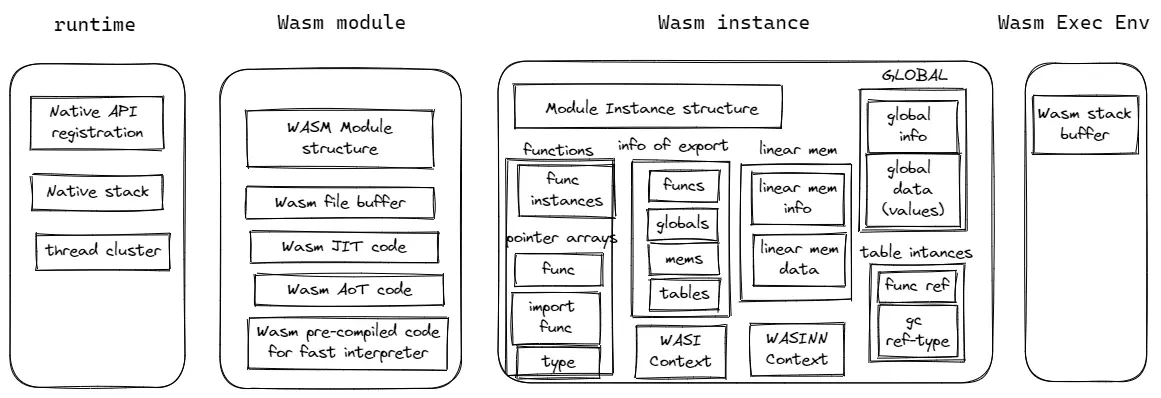
\includegraphics[width=\linewidth]{images/wamr_memory_model.png}
  \caption[WAMR memory layout.]{WAMR memory layout, adapted
  from~\cite{wamr-memory-model}.}
  \label{fig:wamr-memory}
\end{figure}
WAMR's memory consumption is divided into four categories, each with a distinct
lifecycle~\cite{wamr-memory-model}. 

\textbf{Runtime memory} is allocated once during
runtime initialisation and persists for the lifetime of the process, covering internal data
structures for native API registration, the native execution stack, and thread management
state such as pthread wrappers and WASI-thread support.

\textbf{Module memory} is allocated when a \texttt{.wasm} or \texttt{.aot} file is loaded
and freed when the module is unloaded. It includes the parsed \texttt{WASMModule} structure
containing metadata for globals, tables, imports, and exports, as well as a reference to
the file buffer provided by the host. In interpreter mode, this category also includes a
pre-compiled internal bytecode buffer where the fast interpreter converts stack-based Wasm
opcodes into a register-based representation with resolved handler addresses. This
pre-compilation improves dispatch efficiency at runtime but consumes additional memory
proportional to the module's code size --- memory that the AOT path does not require, since
AOT-compiled code is loaded as native machine instructions.

\textbf{Instance memory} is the largest category, allocated when a loaded module is
instantiated into a running instance. It comprises the \texttt{WASMModuleInstance} structure,
function instance metadata, global variable storage, export and table data, and WASI context
state. The most significant sub-allocation is the \textit{linear memory} segment: a
contiguous byte array that the Wasm module uses for all heap allocations and data storage,
with its initial size defined at compile time. The operand stack and application heap are
also allocated at this stage, with their sizes configured as parameters to the instantiation
call.

\textbf{Execution environment memory} provides the calling stack buffer used during Wasm
function execution. It is allocated when a \texttt{wasm\_exec\_env\_t} is created and
released when the execution environment is destroyed after the module's entry point returns.

WAMR supports three allocator modes for managing these categories~\cite{wamr-memory-model}.
\textit{Pool mode} restricts all allocations to a fixed-size buffer supplied by the host at
initialisation, using WAMR's built-in \texttt{ems} allocator. This provides deterministic
memory bounds but requires reserving a sufficiently large contiguous block upfront.
\textit{System allocator mode} delegates all allocations to the platform's standard
\texttt{malloc}/\texttt{free} implementation, allowing WAMR to share the host's
general-purpose heap. \textit{Custom allocator mode} allows the host to supply its own
allocation functions. The choice of allocator mode determines how WAMR's memory consumption
interacts with the rest of the system's heap and has direct implications for the memory
overhead measurements discussed in Chapter~\ref{ch:performance_profiling}.

\subsection{Native Function Interface}
\label{subsec:wamr-host}

A Wasm module cannot directly access hardware peripherals, operating system services, or any resource outside its sandboxed linear memory. All interaction with the external environment occurs through \textit{imported functions}---functions declared by the Wasm module but implemented by the host application. This is the fundamental mechanism by which a Wasm-based control algorithm reads sensor values or actuates outputs. The native functions exposed to the Wasm module communicate strictly using WebAssembly's four primitive numeric types: \texttt{i32}, \texttt{i64}, \texttt{f32}, and \texttt{f64}. Complex data structures, pointers, and strings cannot be passed directly; instead, they are exchanged as \texttt{i32} memory offsets, requiring the host runtime to read or write the corresponding bytes directly within the module's sandboxed linear memory.

In WAMR, native functions are registered as an array of \texttt{NativeSymbol} structures, each specifying a function name, a C function pointer, and a type signature string that encodes the parameter and return types. For example, a host function that returns a floating-point temperature reading is registered with the signature \texttt{"()f"}, indicating no parameters and a float return value. At module instantiation time, WAMR resolves the module's import declarations against the registered symbols.

When a Wasm module calls an imported function, the runtime must perform several operations: decode the \texttt{call} instruction, look up the native symbol, validate the function signature, marshal arguments from the Wasm operand stack to the native C calling convention, invoke the native function, and marshal the return value back onto the Wasm operand stack. Each host function also receives a \texttt{wasm\_exec\_env\_t} parameter providing access to the execution context. This boundary-crossing overhead is a fixed per-call cost that is incurred regardless of the complexity of the underlying native operation, and constitutes a significant portion of the measured overhead in this project's benchmarks, as discussed in Chapter~\ref{ch:performance_profiling}.

\subsection{WAMR Stack Model}
\label{subsec:wamr-stacks}


\begin{figure}[htbp]
      \centering
      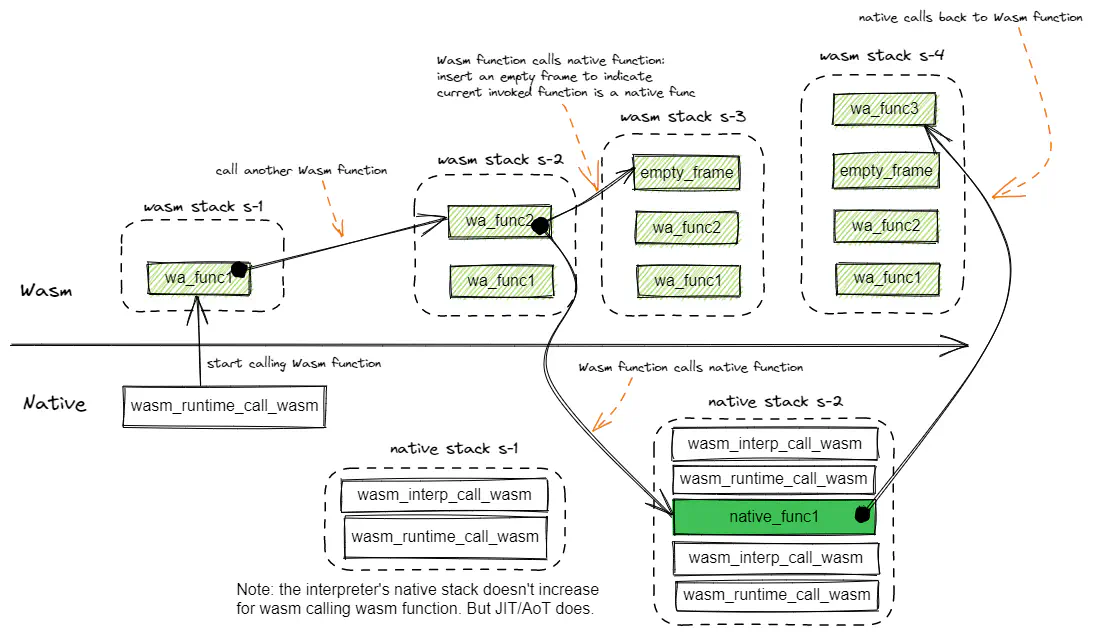
\includegraphics[width=\linewidth]{images/wamr_stack}
      \caption[Interpreter-mode WAMR stack transitions.]{
      Interpreter-mode WAMR stack transitions during Wasm-to-Wasm, Wasm-to-
  native, and native-to-Wasm calls.}
      \label{fig:wamr-interpreter-stacks}
\end{figure}


WAMR uses two distinct notions of stack during execution: the host's native call stack and
the runtime-managed Wasm stack associated with an execution environment
(\texttt{exec\_env})~\cite{wamr-stacks-blog}. The distinction matters because it changes
across execution modes and affects both memory provisioning and call overhead.

In interpreter mode, nested Wasm-to-Wasm calls grow the Wasm stack stored in the
\texttt{exec\_env} stack buffer, while the native stack remains largely unchanged~\cite{wamr-stacks-blog}.
Each interpreter call frame holds the function's locals and operand stack. When control
crosses from Wasm into an imported native function, a native stack frame is created as
usual. If that native function then re-enters Wasm, WAMR inserts an empty marker frame into
the Wasm stack to represent the transition back from native code~\cite{wamr-stacks-blog}.
This behaviour is directly relevant to the host-call measurements in \autoref{ch:performance_profiling} 
because the observed interpreter overhead includes not only the native function body but
also the bookkeeping required to move between WAMR's interpreter stack representation and
the host C calling convention.

In AOT and JIT modes, ordinary Wasm call frames are integrated into the runtime's native
stack frames rather than being stored in a separate interpreter stack buffer~\cite{wamr-stacks-blog}.
Each Wasm function call therefore grows the native stack in the conventional way. The
\texttt{exec\_env} object still provides the execution context passed to imported functions,
but its dedicated stack buffer is used much less heavily and is primarily retained for
optional diagnostics such as call-stack or profiling dumps~\cite{wamr-stacks-blog}. This
different stack organisation is one reason why AOT execution reduces runtime overhead
relative to interpretation.

In this project, the controller firmware instantiates each module with a \texttt{16~KiB}
default stack parameter and then invokes the module's entry point through an explicitly
created \texttt{exec\_env} with an \texttt{8~KiB} stack buffer. 

\subsection{Execution Modes}
\label{subsec:wamr-modes}

The \texttt{iwasm} VM core supports multiple execution modes, each representing a different
trade-off between execution performance, memory consumption, startup latency, and platform
requirements~\cite{wamr-running-modes-blog, wamr-running-modes-doc}. These modes are
selectively compiled into the runtime binary via CMake build flags, and the execution mode
for a given module instance can be controlled at runtime through WAMR's embedding API.

\paragraph{Interpreter mode:} WAMR provides two interpreter variants, selected at compile
time via the \texttt{WAMR\_BUILD\_FAST\_INTERP} flag; they cannot coexist in the same
binary. The \textit{Classic Interpreter} is a straightforward stack-based bytecode
interpreter that walks the Wasm opcode stream and dispatches each instruction at runtime. It
has the smallest memory footprint of all execution modes and is currently the only mode that
supports WAMR's source-level debugging facilities~\cite{wamr-running-modes-blog}. The
\textit{Fast Interpreter} pre-compiles the Wasm bytecode into an internal opcode format
during module loading, resolving handler addresses and fusing common opcode sequences into a
register-based internal representation. The official WAMR documentation reports that the
Fast Interpreter runs approximately twice as fast as the Classic Interpreter, at the cost of
additional memory to hold the pre-compiled code~\cite{wamr-running-modes-doc,
wamr-fast-interp}. Both interpreters require no executable memory regions, making them
suitable for platforms without an MMU or with execute-in-place flash memory. This project
uses the Fast Interpreter, as it provides the stronger performance baseline for evaluating
interpreter overhead against native execution.

\paragraph{Ahead-of-Time (AOT) compilation:} The \texttt{wamrc} compiler compiles a
\texttt{.wasm} binary offline into a native machine code file (\texttt{.aot}) for a
specific ISA, using LLVM as its backend. At runtime, the \texttt{iwasm} VM core's AOT
module loader (enabled with \texttt{WAMR\_BUILD\_AOT=1}) loads the \texttt{.aot} file,
performs relocation, and links the compiled native code with the host's registered imported
functions~\cite{wamr-running-modes-blog}. Because control flow, register allocation, and
instruction selection are resolved at compile time, AOT execution achieves near-native speed
with very small runtime footprint and quick startup~\cite{wamr-running-modes-doc}. The AOT
loader can coexist with any interpreter or JIT engine in the same binary. The trade-off is
that the \texttt{.aot} file is architecture-specific --- a separate \texttt{wamrc}
invocation is required for each target ISA --- partially sacrificing Wasm's portability
advantage.

\paragraph{Just-in-Time (JIT) compilation:} WAMR supports two JIT tiers. The \textit{Fast
JIT} is a lightweight engine implemented with a self-contained code generator, offering
quick startup and small footprint but currently limited to x86-64 targets on Linux,
Linux-SGX, and macOS. Its performance is approximately 50\% that of LLVM
JIT~\cite{wamr-running-modes-doc}. The \textit{LLVM JIT} uses the full LLVM compilation
framework and delivers the best JIT execution performance --- approximately twice that of
Fast JIT --- at the cost of longer compilation latency~\cite{wamr-running-modes-blog}. WAMR
also supports dynamic \textit{tier-up}: a module can begin execution under Fast JIT for
rapid cold start and transparently switch to LLVM JIT-compiled code as it becomes available,
combining quick startup with high steady-state performance. However, both JIT modes require
the ability to allocate and execute dynamically generated machine code at runtime, which is
unavailable on microcontrollers such as the ESP32 that lack an MMU and do not support
executable heap memory. JIT compilation is therefore not used in this project.

\paragraph{Mode selection rationale:} This project evaluates both the Fast Interpreter and
AOT modes. The Fast Interpreter represents the most portable deployment scenario: a single
\texttt{.wasm} binary can be distributed to any WAMR-supported platform and executed
without a separate compilation step. AOT represents the highest-performance scenario, where
the Wasm module is pre-compiled for the ESP32's Xtensa LX6 architecture using
\texttt{wamrc} before being flashed to the device. Comparing both modes against native C
execution reveals the overhead attributable to the Wasm abstraction layer at each end of the
performance--portability spectrum.

% ------------------------------------------------------------
\section{ESP32 Hardware Platform}
\label{sec:esp32}
% ------------------------------------------------------------

\subsection{Xtensa LX6 Dual-Core Architecture}
\label{subsec:xtensa}

The ESP32 is a system-on-chip (SoC) designed by Espressif Systems, widely used in IoT and embedded applications. It features a dual-core Xtensa LX6 processor running at up to 240~MHz, 520~KB of on-chip SRAM, and integrated Wi-Fi and Bluetooth connectivity~\cite{esp32-trm}. The two CPU cores share access to the same SRAM through a common memory bus, with each core maintaining its own instruction cache (32~KB per core) but sharing the data bus and peripheral bus.

The shared memory bus architecture is significant for this project's analysis. When both cores actively access memory, bus arbitration introduces contention that can increase access latency for both cores. This effect is normally negligible in typical IoT workloads where one core is often idle, but becomes relevant when the WAMR interpreter on one core performs intensive, irregular memory access patterns such as bytecode fetch, operand stack manipulation, and indirect dispatch table, lookups, while the other core simultaneously reads ADC values and traverses FreeRTOS kernel data structures.

The ESP32 lacks a memory management unit (MMU) in the conventional sense---there is no virtual memory or page-based memory protection. All tasks share a single flat address space, and memory protection relies on the RTOS and application-level discipline rather than hardware enforcement. This absence of an MMU is one reason why Wasm's software-enforced memory sandboxing is particularly valuable on this platform: it provides memory isolation guarantees that the hardware cannot.



\subsection{Flash and Execute-in-Place (XIP)}
\label{subsec:esp32-xip}

The ESP32 has 520\,kB of on-chip SRAM but keeps firmware in a much larger external SPI flash chip; the DevKitC boards used in this project carry 4\,MB~\cite{esp32-trm}. Rather than copying code into SRAM at boot, the processor executes directly out of flash through a memory-mapped cache, an arrangement known as execute-in-place (XIP). Applications can therefore ship binaries that are larger than the available RAM, but instruction fetches now depend on what the cache holds.

The cache maps 32\,kB regions of flash into the instruction address space on demand. A fetch to an already-resident region costs the same as an SRAM access; a fetch to a non-resident region stalls the CPU while the controller reads the region from flash. Code with good locality almost never pays that price. Code with poor locality, such as the indirect dispatch loop of a Wasm interpreter, accumulates enough misses to show up as measurable execution overhead. The \texttt{.rodata} section is mapped through the data cache on the same principle. Only \texttt{.bss}, \texttt{.data}, task stacks, and the heap live permanently in on-chip SRAM.

\subsection{GPIO and Analogue I/O}
\label{subsec:esp32-gpio}

The ESP32 exposes 34 GPIO pins, many of them multiplexed with peripheral functions including SPI, I\textsuperscript{2}C, UART, PWM, and analogue conversion~\cite{esp32-trm}. Of particular relevance to this project are the on-chip analogue peripherals. The SoC provides two 12-bit successive-approximation ADC units for voltage sampling and two 8-bit DAC channels for analogue output, all referenced to the 3.3\,V supply. The ADC is used when the microcontroller needs to read an external analogue signal, such as a sensor voltage, and convert it into a digital value that software can work with. The DAC does the reverse: it lets software produce a voltage level that can be sent to other analogue components. This makes the ESP32 suitable for simple low-cost sensing and actuation tasks without requiring external converter hardware. Figure~\ref{fig:esp32-pinout} gives an overview of the available pin functions on the ESP32-DevKitC used in the testbed. The specific pin assignments and signal roles used in the experimental testbed are described later in Chapter~\ref{ch:design}.

\begin{figure}[htbp]
    \centering
    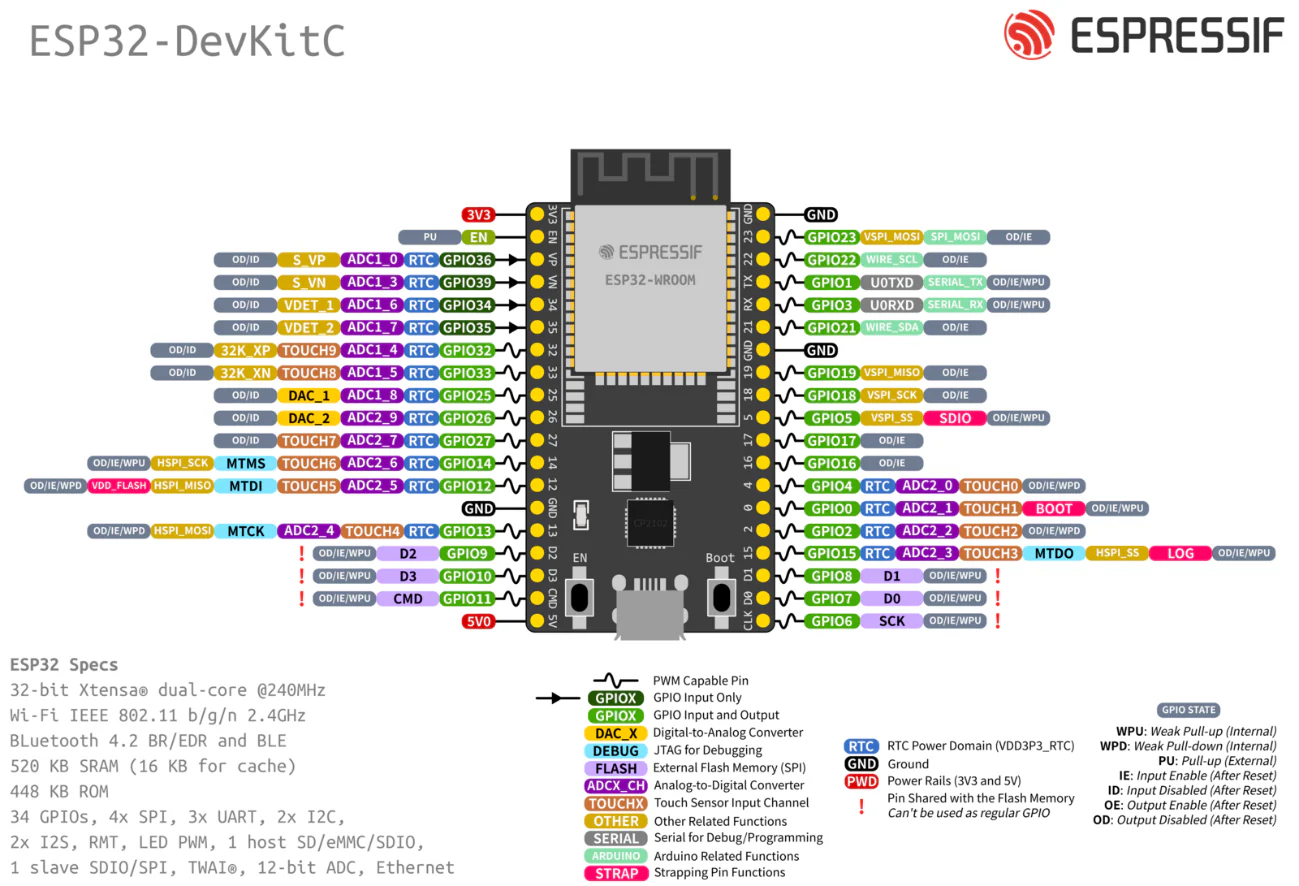
\includegraphics[width=0.92\textwidth]{images/esp32_pinout.png}
    \caption{ESP32-DevKitC pinout overview, showing the range of GPIO, ADC, DAC, and peripheral functions exposed by the board.}
    \label{fig:esp32-pinout}
\end{figure}

\subsection{SPI Flash File System (SPIFFS)}
\label{subsec:esp32-spiffs}

SPIFFS is a lightweight filesystem designed for flash storage on microcontrollers~\cite{spiffs}. It treats a flash partition as a flat namespace of small files and handles wear levelling and power-loss tolerance internally, without a directory tree. ESP-IDF ships a SPIFFS component that mounts a named partition at a user-chosen path (\texttt{/spiffs} in this project) and exposes it through the standard POSIX file API.

For the containerised setup, the partition table dedicates a 512\,kB SPIFFS region at offset \texttt{0x210000} to the Wasm binaries. At build time the container files in \texttt{wasm\_assets/} are packed into an image (\texttt{storage.bin}) and written into this region by \texttt{esptool}. At runtime WAMR opens the relevant \texttt{.wasm} or \texttt{.aot} file by path, streams it into RAM, and hands the bytes to its loader. Because the containers live on a separate partition from the application binary, a field update that only swaps the containers never touches the bootloader or the firmware. Chapter~\ref{ch:containerization_strategy} uses exactly this boundary for the SPIFFS-only OTA path.

\section{FreeRTOS}
\label{subsec:freertos}

FreeRTOS is an open-source real-time operating system kernel widely used in embedded
systems~\cite{freertos-esp}. It provides preemptive multitasking on resource-constrained
hardware, allowing multiple concurrent tasks to share a single processor through
priority-based scheduling. Each task is assigned a fixed priority level, and the scheduler
always selects the highest-priority ready task for execution. Tasks of equal priority are
scheduled round-robin within configurable time slices. When no application task is ready to
run, the scheduler executes a low-priority idle task.

Tasks in FreeRTOS are created with a fixed-size stack allocated from the heap at creation
time. Unlike general-purpose operating systems, there is no virtual memory or dynamic stack
growth --- the developer must specify a stack size at task creation that is sufficient for
the task's worst-case call depth. Inter-task communication and synchronisation are provided
through primitives including binary and counting semaphores, mutexes with priority
inheritance (to prevent unbounded priority inversion), message queues, and event
groups~\cite{astrom-feedback}.

The standard FreeRTOS kernel is designed for single-core processors. For multi-core targets
such as the ESP32, ESP-IDF provides a modified implementation that extends the kernel with
symmetric multiprocessing (SMP) support~\cite{freertos-esp}. This extension introduces the
ability to pin tasks to a specific core using
\texttt{xTaskCreatePinnedToCore()}, ensuring that a task always executes on a designated
core rather than being migrated by the scheduler. Each core maintains its own idle task, and
the scheduler independently selects the highest-priority ready task on each core.

FreeRTOS also provides facilities for runtime instrumentation. When runtime statistics
collection is enabled, a high-resolution hardware timer accumulates per-task tick counts that
record how much CPU time each task has consumed. The kernel function
\texttt{uxTaskGetSystemState()} returns these counters for all tasks in the system, from
which per-core CPU utilisation can be derived by comparing the idle task's accumulated ticks
against the total elapsed time over a measurement interval.

\section{ESP-IDF Development Framework}
\label{subsec:esp-idf}

ESP-IDF (Espressif IoT Development Framework) is the official open-source SDK for
Espressif's ESP32 family of SoCs~\cite{esp-idf-docs, esp-idf-github}. Written primarily in
C and licensed under Apache 2.0, it provides peripheral drivers, networking stacks (Wi-Fi,
Bluetooth, TCP/IP), file system support, cryptographic libraries, and a build system for
cross-compiling firmware targeting the ESP32's Xtensa architecture.

FreeRTOS is integrated into ESP-IDF as a core component rather than as a separate operating
system layer~\cite{freertos-esp}. The version shipped with ESP-IDF is based on Vanilla
FreeRTOS v10.5.1 but includes significant modifications to support symmetric multiprocessing
on the ESP32's dual cores. All ESP-IDF applications --- including both controllers in this
project --- are built against this SMP-aware FreeRTOS API.

The framework uses a CMake-based build system organised around reusable
\textit{components}. Third-party libraries such as WAMR are added as managed components and
compiled alongside the core framework automatically. Compile-time configuration is managed
through \texttt{idf.py menuconfig}, which exposes options for FreeRTOS kernel settings
(tick rate, runtime statistics collection), peripheral drivers, and WAMR-specific options
such as interpreter variant and AOT loader enablement. The application entry point is a
user-defined \texttt{app\_main()} function called automatically after the scheduler and core
peripherals have been initialised~\cite{freertos-esp}. Both the native and WAMR controllers
in this project define their task topology and begin execution from within
\texttt{app\_main()}.



% \subsection{Peripheral Interfaces}
% \label{subsec:peripherals}

% The ESP32's on-chip peripherals relevant to this project are the digital-to-analogue converter (DAC) and analogue-to-digital converter (ADC). The DAC provides two 8-bit output channels (GPIO~25 and GPIO~26), each capable of producing a voltage between 0 and approximately 3.3~V with 256 discrete levels. The ADC provides two units (ADC1 and ADC2) with 12-bit resolution (4096 levels). ADC1 channels are available on GPIOs~32--39; ADC2 channels share pins with the Wi-Fi peripheral and are therefore less reliable when Wi-Fi is active.

% The 8-bit DAC resolution limits the heater command to 256 discrete power levels, and the 12-bit ADC resolution limits temperature readings to approximately 0.08\textdegree C per least significant bit (assuming a 0--100\textdegree C mapping over the full 3.3~V range). These quantisation effects introduce a noise floor into both the control signal and the measured temperature, which is an inherent characteristic of the analogue signal path between boards.

% ADC readings are performed using the \texttt{adc\_oneshot} driver in ESP-IDF, which configures the channel attenuation and bit width, performs a single conversion, and returns the raw digital value. Calibration is applied using ESP-IDF's line-fitting calibration scheme, which corrects for per-chip manufacturing variations by reading factory-programmed reference voltage values from the chip's eFuse memory. The calibrated output is a voltage in millivolts, which the reader task converts to a temperature using a linear scaling based on the simulator's known voltage-to-temperature mapping.

% ------------------------------------------------------------
\section{Real-Time Control Fundamentals}
\label{sec:control}
% ------------------------------------------------------------

\subsection{Closed-Loop Control and Timing Requirements}
\label{subsec:closed-loop}

A closed-loop (feedback) control system continuously measures the output of a physical process, compares it to a desired setpoint, and adjusts an actuator to minimise the error. The control loop operates at a fixed period $T$, typically ranging from sub-millisecond (for motor control) to seconds (for thermal processes). At each period, the controller reads the sensor, computes the control action, and writes the actuator command.

Two timing properties are critical for correct control behaviour. The \textit{control period} $T$ must be short enough to capture the dynamics of the controlled process---the Nyquist criterion requires sampling at least twice the bandwidth of the fastest disturbance, though practical control systems typically sample 10--20 times faster~\cite{astrom-feedback}. The \textit{jitter} in the control period---the variation in the actual time between successive control actions---must be small relative to $T$, as jitter introduces a time-varying phase shift that can degrade stability margins and increase overshoot.

For the thermal system modelled in this project, with a heating rate of 2.0\textdegree C/s and a cooling time constant of several seconds, even a 10~Hz loop is sufficient for stable control. The tighter 100~Hz case used in the step-response workload is therefore deliberate over-sampling rather than a control-theoretic requirement. It shrinks the time budget to 10~ms per iteration and makes any per-iteration runtime overhead directly visible in the timing measurements.

\subsection{Bang-Bang and PID Controllers}
\label{subsec:controllers}

\paragraph{Bang-bang control.} The simplest form of closed-loop control is hysteresis (bang-bang) control, where the actuator is driven fully on or fully off depending on whether the measured temperature is below or above the setpoint. A hysteresis band of $\pm\delta$ around the setpoint prevents rapid switching (chattering) near the target. If $T_{\text{measured}} < T_{\text{target}} - \delta$, the heater is set to full power; if $T_{\text{measured}} > T_{\text{target}} + \delta$, the heater is turned off. Within the hysteresis band, the previous actuator state is maintained. This controller requires negligible computation per iteration, making it useful as a baseline for isolating runtime overhead from algorithmic complexity.

\paragraph{PID control.} The proportional-integral-derivative (PID) controller computes the actuator command $u(t)$ as a weighted sum of three terms derived from the error signal $e(t) = T_{\text{target}} - T_{\text{measured}}$:

\begin{equation}
\label{eq:pid}
u(t) = K_p \, e(t) + K_i \int_0^t e(\tau) \, d\tau + K_d \, \frac{de(t)}{dt}
\end{equation}

\noindent where $K_p$ is the proportional gain (responding to the current error), $K_i$ is the integral gain, and $K_d$ is the derivative gain. In discrete time with sampling period $T$, the integral is approximated by a running sum and the derivative by a first-order difference:

\begin{equation}
\label{eq:pid-discrete}
u[k] = K_p \, e[k] + K_i \, T \sum_{j=0}^{k} e[j] + K_d \, \frac{e[k] - e[k-1]}{T}
\end{equation}

Anti-windup clamping is applied to the integral term to prevent accumulation of error during actuator saturation, bounding the integral between configurable limits $[I_{\min}, I_{\max}]$. The output $u[k]$ is clamped to the range $[0, 1]$ before being written to the DAC as a heater power fraction.

Like bang-bang control, the PID computation is arithmetically simple (a few multiplications and additions per iteration) and completes in microseconds on a 240~MHz processor. The dominant cost per control loop iteration is not the algorithm itself but the sensor read, actuator write, and any runtime overhead---which is precisely what this project measures.

% ------------------------------------------------------------
\section{Related Works}
\label{sec:related}

Research on WebAssembly in embedded and IoT environments has grown considerably since
Wasm's standardisation, though comparatively few studies have examined real-time control
applications specifically. \\

\textbf{WARDuino }a
WebAssembly virtual machine designed for Arduino-compatible
microcontrollers~\cite{warduino2024}. WARDuino extends the standard Wasm VM with remote
debugging, over-the-air reprogramming, and hardware access primitives. Their benchmarks
showed WARDuino to be approximately 426 times slower than native C execution and 38 times
slower than WASM3 (an AOT-capable runtime), but 12 times faster than Espruino, a JavaScript
interpreter for ESP32. While WARDuino demonstrates the feasibility of running Wasm on
microcontrollers, it is a pure interpreter without AOT support, and its benchmarks focused
on micro-benchmarks (such as a breakout game) rather than closed-loop control workloads. \\

A recent study evaluated both WAMR and wasm3 in interpreter mode on three microcontrollers:
the Raspberry Pi Pico (ARM Cortex-M0+), ESP32-C6 (RISC-V), and nRF5340
(ARM Cortex-M33)~\cite{wasm-iot-constrained}. Using bubble sort and CRC-16 workloads, they
found that on the Pico a 1000-element bubble sort took approximately 612~\textmu{}s
natively, 6,358~\textmu{}s under wasm3 (a 10.4x slowdown), and 29,475~\textmu{}s under
WAMR (a 48x slowdown). Wasm execution was also 10--40 times more energy-hungry than native
code across all devices. The authors concluded that Wasm offers acceptable trade-offs when
portability and sandboxing outweigh strict performance constraints, but noted that only
interpreter mode was tested and that AOT and JIT evaluation remained as future
work --- a gap that the present project partially addresses. \\

Moron and Wallentowitz conducted the most
comprehensive embedded Wasm benchmarking study to date, comparing WAMR (classic and fast
interpreter), wasm3, WARDuino, and Wasmi against Lua and MicroPython on an STM32L4
Cortex-M4 microcontroller using the \textbf{Embench} benchmark suite~\cite{moron2025benchmarking}.
Across all benchmarks, wasm3 was the fastest interpreter at 36.9x native execution time
($\sigma = 8.0$), closely followed by WAMR's fast interpreter at 43.3x ($\sigma = 10.9$).
Both substantially outperformed Lua at 176x ($\sigma = 116.0$) and MicroPython at 636x
($\sigma = 575.5$). When AOT compilation was enabled, WAMR reduced the overhead to just
2.2--2.4x native, demonstrating that the compilation step can nearly eliminate the
interpreter penalty. Their memory analysis showed WAMR's total memory footprint (static plus
dynamic) to be approximately 5x that of native code, comparable to MicroPython and lower
than Lua's 8x. The authors concluded that WebAssembly is preferable to alternative embedded
VMs, offering competitive performance with greater language flexibility and stronger
isolation guarantees. However, their evaluation used computational benchmarks on a
single-core platform and did not examine real-time control workloads, multi-core scheduling
effects, or host function call overhead --- all of which the present project addresses. \\

Rausch et al.\ conducted a
cross-architecture evaluation of Wasm using Wasmtime and WAMR across ARM, x86, and RISC-V
platforms~\cite{rausch2024cross}. Their characterisation of standalone runtimes found that
interpreter execution introduced an average 1.59x to 9.57x performance slowdown relative to
native code, with the range depending heavily on the workload and target architecture. AOT
compilation substantially closed this gap, bringing execution time and startup latency close
to native levels on all tested platforms. However, their evaluation targeted server-class
and single-board computer hardware rather than microcontrollers, and did not examine
real-time constraints or memory-limited environments. \\


% \paragraph{Real-time and embedded Wasm.} Research specifically addressing Wasm in real-time
% contexts is limited. Seidler et al.\ proposed Wasm-IO, a set of WASI interfaces for
% low-level device interaction in industrial automation, addressing the gap between Wasm's
% sandboxed execution model and the direct hardware access required by control
% systems~\cite{seidler2025wasmio}. Their work highlights the standardisation challenge but
% does not benchmark execution overhead. The Bytecode Alliance established an Embedded Special
% Interest Group (ESIG) in 2024 to address requirements specific to the embedding industry
% --- prioritising performance, footprint, and stability over the cloud-centric features that
% dominate the broader Wasm standardisation effort~\cite{wamr-2024-review}.

Prior work has established that Wasm can execute on microcontrollers and that AOT compilation
approaches native speed. However, no study has benchmarked Wasm in a closed-loop real-time
control context with millisecond-scale timing budgets, compared interpreter and AOT modes
under such constraints, or investigated the system-level effects of a Wasm runtime on
multi-core RTOS scheduling. This project addresses these gaps on ESP32 hardware.




% ============================================================
\chapter{Design and Implementation}
\label{ch:design}
% ============================================================

This chapter sets out the common platform used by the three evaluation chapters: performance profiling (Chapter~\ref{ch:performance_profiling}), fault tolerance (Chapter~\ref{ch:fault_tolerance}), and containerisation strategies (Chapter~\ref{ch:containerization_strategy}). It covers the two-board testbed, the thermal simulator, the controller firmware structure, the WebAssembly toolchain, and the runtime initialisation sequence. The later chapters vary the workload or deployment strategy while keeping this shared base fixed.

The application modelled by the testbed is a closed-loop thermal-control system. One ESP32 board simulates the thermal plant, including the heating element, thermistor response, sampling delay, and analogue quantisation. A second ESP32 board runs the controller, reads the simulated temperature, and drives the simulated heater. A thermal process was chosen because it is slow enough to control reliably on an ESP32-class device while still exercising the features that matter for embedded control: periodic sensing, actuation, state feedback, timing delay, and repeatable plant dynamics.

The native and WAMR controller firmware share the same FreeRTOS task topology, ADC and DAC paths, and capture pipeline. The design goal is to make the execution environment the only meaningful independent variable, so that later differences in latency, memory footprint, fault behaviour, or inter-container communication overhead can be traced back to the WebAssembly runtime rather than to incidental implementation differences.

For this reason, the chapter includes implementation details that might otherwise appear low-level. Task placement, signal routing, memory allocation, host-function boundaries, and reset behaviour all affect the timing, memory, and fault-containment results reported later. Making these details explicit shows that the native and containerised variants are functionally and structurally matched before their performance is compared.

% ------------------------------------------------------------

% ------------------------------------------------------------
\section{Execution Variants: Native vs WAMR}
\label{sec:variants}
% ------------------------------------------------------------

The Controller board is evaluated using a native firmware baseline and a containerised WAMR firmware. The WAMR firmware is used in two execution modes in the later experiments: interpreter mode and AOT mode.

\paragraph{Native Variant:} This is the baseline. The control algorithms are compiled by the ESP-IDF toolchain directly into Xtensa LX6 machine code. The resulting application is a monolithic firmware binary in which the control loop runs as a normal FreeRTOS task with direct access to hardware peripherals and the RTOS API.

\paragraph{WAMR Variant:} This is the containerised design, covering both the WAMR interpreter and WAMR AOT runs used in the evaluation. The same control logic is implemented with matched constants, control flow, and host-facing calls, then compiled with \texttt{wasi-sdk} into an architecture-agnostic WebAssembly module. For AOT runs, this module is then compiled offline into an Xtensa-specific \texttt{.aot} file. The ESP-IDF firmware acts as the host, launching the WebAssembly Micro Runtime (WAMR) inside a FreeRTOS pthread. The control loop then runs inside WAMR's software sandbox and reaches the hardware only through host functions.

Because the surrounding firmware is otherwise kept the same, any measured differences in latency, footprint, or fault tolerance can be attributed to the runtime rather than to a different controller architecture.


\section{The Testbed}
\label{sec:arch-overview}

\begin{figure}[htpb]
    \centering
    \begin{subfigure}[t]{0.38\textwidth}
        \centering
        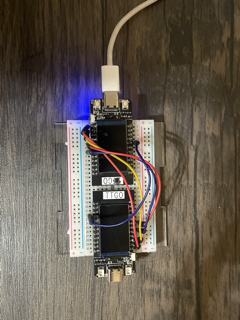
\includegraphics[height=0.30\textheight]{images/testbed_picture.png}
        \caption{Physical testbed.}
    \end{subfigure}
    \hfill
    \begin{subfigure}[t]{0.58\textwidth}
        \centering
        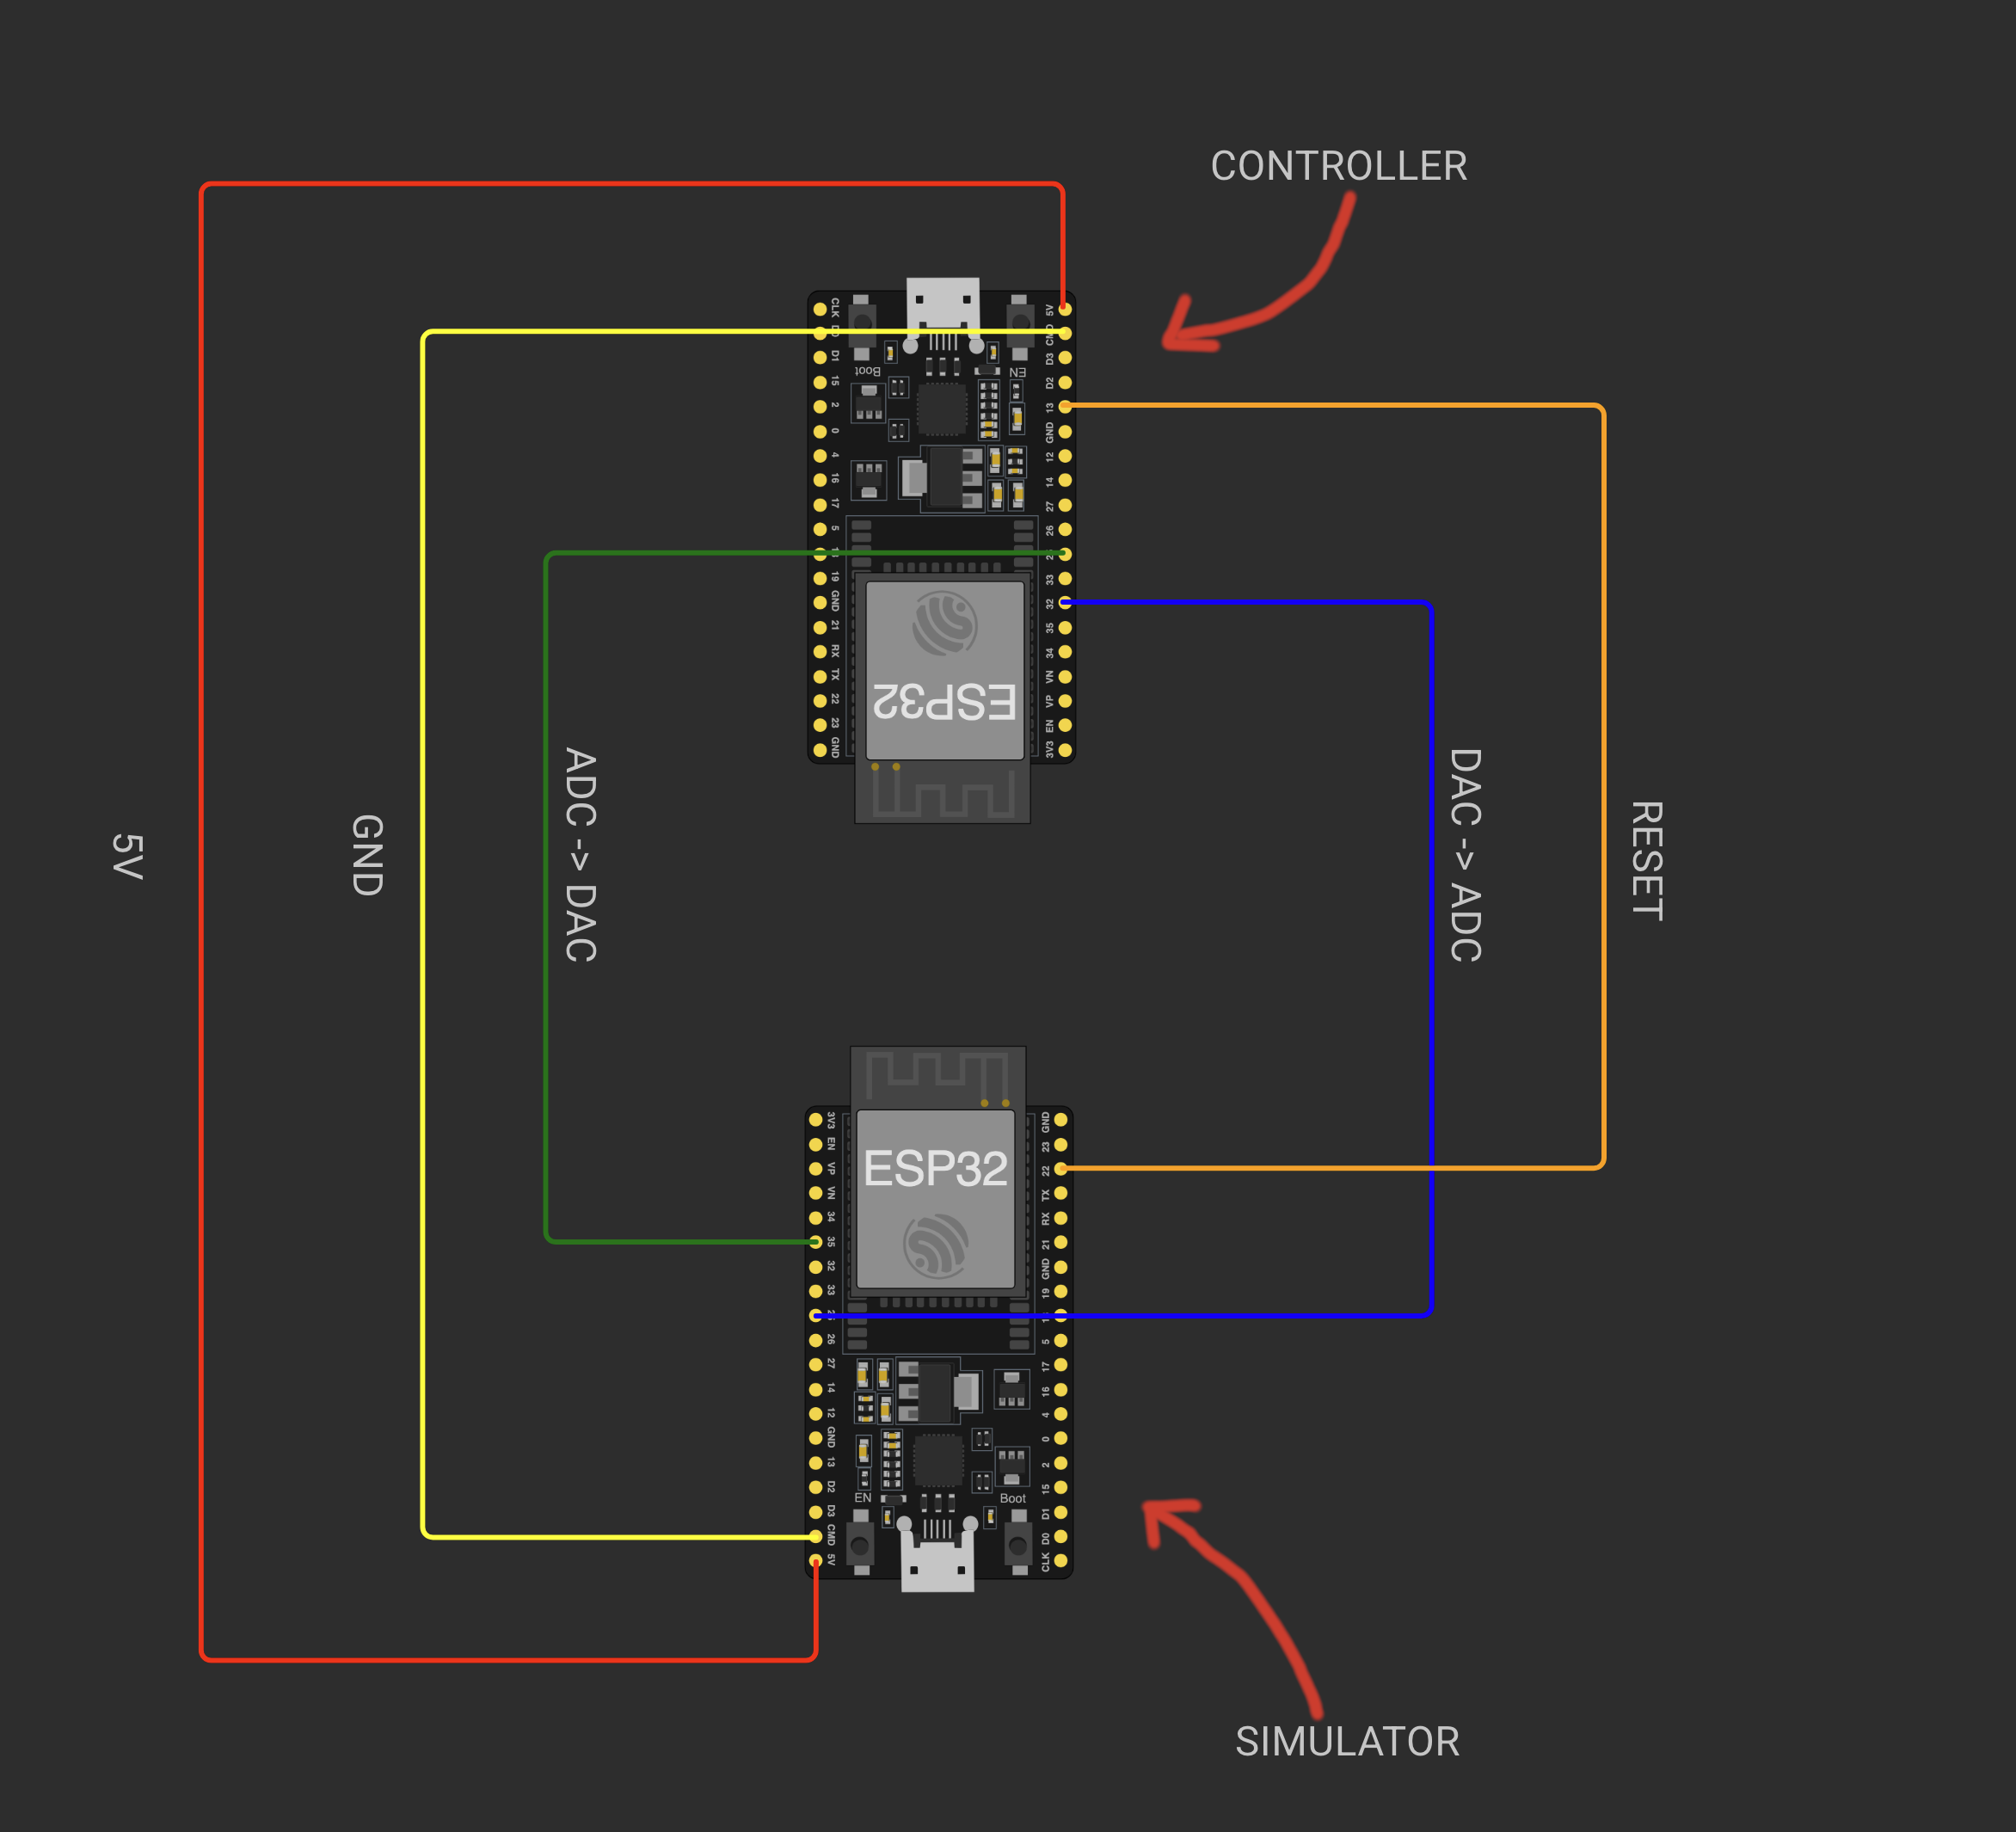
\includegraphics[height=0.30\textheight]{images/circuit_diagram_annotated.png}
        \caption{Connection diagram.}
    \end{subfigure}
    \caption{Physical testbed and wiring layout.}
    \label{fig:testbed}
\end{figure}

Figure~\ref{fig:testbed} shows the physical testbed and the corresponding connection layout. The experimental setup consists of two ESP32 development boards connected by GPIO jumper wires to emulate the signal paths of a closed-loop thermal control system. One board acts as the \textbf{Thermal Simulator}, running a fixed physics model throughout all experiments. The second board acts as the \textbf{Controller}, which is reflashed between test runs with either the native C or WAMR firmware variants. The boards are linked by two analogue signal paths for heater and temperature exchange, and by a separate digital reset connection used to return the simulator to ambient before each run.

The Simulator board hosts a digital twin of a thermal environment. It updates the plant state from the received heater command and returns the resulting sensor value as an analogue voltage. This Hardware-in-the-Loop (HIL) arrangement keeps the experiment repeatable while still preserving the delays, quantisation, and asynchronous behaviour that disappear in a purely software-based simulation.

The signal flow operates as follows:

\begin{enumerate}
    \item The Controller reads the current temperature via its ADC on \textbf{GPIO~32}, computes a
    control action, and writes a heater command via its DAC on \textbf{GPIO~25}.
    \item The analogue heater command propagates over a wire to the Simulator's ADC
    on \textbf{GPIO~32}, where it is read as a heater power fraction.
    \item The Simulator updates its physics model, computes a new temperature, and outputs
    it via its DAC on \textbf{GPIO~25}.
    \item The analogue temperature signal propagates back to the Controller's ADC, closing 
    the loop.
    \item Between runs, the Controller pulses a reset signal on \textbf{GPIO~13}, the Simulator monitors this line on \textbf{GPIO~22}, and its internal temperature state is reset to ambient.
\end{enumerate}

This architecture uses the DAC-to-ADC analogue signal path rather than a digital bus (such
as SPI or I\textsuperscript{2}C) to introduce realistic signal propagation delays and
quantisation effects, making the end-to-end latency measurements closer to a physical
signal path than an idealised software-only simulation. The reset line serves a different purpose, ensuring that every run begins from the same thermal baseline without reflashing or power-cycling the Simulator board. Because the same boards, wiring, and support tasks are used for every variant, measured differences can be tied back to the firmware rather than to hardware variation.



% ------------------------------------------------------------
\section{Thermal Simulator}
\label{sec:simulator}
% ------------------------------------------------------------

\subsection{Physics Model}
\label{subsec:physics}

The simulator models a simplified thermal plant consisting of a heater and a temperature sensor in a thermally coupled enclosure. The state variable is the current temperature $T$, which evolves according to a first-order energy balance. At each simulation tick, the heater power $P \in [0, 1]$ is read from the ADC, and the temperature is updated as:

\begin{equation}
\label{eq:physics}
T_{\text{next}} = \alpha \cdot T + (1 - \alpha) \cdot \left( T + P \cdot R_{\text{heat}} - (T - T_{\text{amb}}) \cdot R_{\text{cool}} \right)
\end{equation}

\noindent where $\alpha = 0.7$ is the thermal mass (an inertia parameter that smooths transients), $R_{\text{heat}} = 2.0$\textdegree C per tick is the heating rate at full power, $R_{\text{cool}} = 0.02$ is the cooling coefficient, and $T_{\text{amb}} = 25.0$\textdegree C is the ambient temperature. The temperature is clamped to $[T_{\text{amb}}, 100.0]$\textdegree C. When sensor noise is enabled (for non-end-to-end tests), a uniform random offset in the range $\pm 0.3$\textdegree C is added to the output.

This model is intentionally simple. It captures the essential dynamics of a thermal system --- heating, cooling, and thermal inertia --- without introducing complexity that would obscure the benchmarking objectives. The parameters were tuned empirically to produce a response that is fast enough to generate measurable temperature changes within the 3-second heating windows used by the step-response algorithm, while still exposing the discrete timing effect of the simulator's 50~ms update period.

\subsection{Simulation Loop}
\label{subsec:sim-loop}

The simulator runs a single task in \texttt{app\_main()} that executes at 20~Hz (50~ms
period via \texttt{vTaskDelay(pdMS\_TO\_TICKS(50))}). Each iteration reads the heater power
from the ADC, updates the physics model ($T$), and outputs the resulting temperature via the
DAC. The ADC is configured on GPIO~32 using the \texttt{adc\_oneshot} driver with 12-bit
resolution and 12~dB attenuation, with line-fitting calibration applied via eFuse reference
voltages. The DAC outputs on GPIO~25 with 8-bit resolution, mapping the temperature range
$[0, 100]$\textdegree C to the $[0, 255]$ DAC output range.

The 20~Hz tick rate was chosen to reflect the response characteristics of a real thermal
plant, where sensors and actuators do not update synchronously with the controller. In
industrial control systems, the round-trip latency between a controller issuing a command
and receiving a sensor update is typically 10--50~ms due to fieldbus communication
delays, sensor response times, and actuator settling~\cite{sealevel-sampling}.

\subsection{Simulator Reset Mechanism}
\label{subsec:sim-reset}

Consecutive benchmark runs can leave residual heat in the simulated thermal environment, causing subsequent experiments to begin from an elevated baseline rather than ambient. To ensure each run starts from a known initial state, a GPIO-based reset signal is used between the two boards. Before each algorithm run, the controller pulses GPIO~13 high, then waits 2~seconds for the system to stabilise. The simulator monitors GPIO~22 (configured as input with pull-down) and resets its internal temperature to $T_{\text{amb}} = 25.0$\textdegree C when the signal is detected. This mechanism is invoked during start-up of both controller variants before any workload begins.

% ------------------------------------------------------------
\section{System Tasks}
\label{sec:tasks}
% ------------------------------------------------------------

Both controller variants rely on a common set of concurrent FreeRTOS tasks that handle sensor acquisition, system monitoring, and data logging independently of the main control or workload task. These support tasks are implemented identically in the native and WAMR firmware, ensuring that any measured differences originate from the execution environment rather than the surrounding infrastructure. The specific workload task varies by experiment and is described in the corresponding evaluation chapter. Depending on the experiment, it may be a control algorithm, a fault-injection routine, or an inter-container communication (IPC) benchmark.

\subsection{ADC Reader Task}
\label{subsec:native-reader}

A dedicated reader task is pinned to Core~1 at priority~5. It initialises the ADC on GPIO~32 with 12-bit resolution and 12~dB attenuation, applies line-fitting calibration, and enters a continuous loop whose sampling rate is matched to the workload's control period (typically 100~ms). Each iteration performs an \texttt{adc\_oneshot\_read()}, converts the raw value to millivolts via \texttt{adc\_cali\_raw\_to\_voltage()}, and maps the voltage to a temperature using the linear relationship:

\begin{equation}
\label{eq:temp_conversion}
T = \left( \frac{V_{\text{mV}}}{3300} \right) \times 100 \, ^\circ\text{C}
\end{equation}

The reader task updates the shared \texttt{current\_temp} variable under \texttt{temp\_mutex} and records the ADC read timing, free heap size, and mutex wait times under \texttt{metrics\_mutex}. It also implements the end-to-end detection logic: when the \texttt{waiting\_for\_rise} flag has been set by \texttt{set\_heater()} and the measured temperature exceeds \texttt{temp\_at\_command} by more than the \texttt{E2E\_THRESHOLD} (configured as 0.5\textdegree C), the reader records the end-to-end delay as the difference between the current time and \texttt{command\_send\_time\_us}, and clears the flag.

\subsection{CPU Usage Task}
\label{subsec:native-cpu}

A CPU measurement task runs on Core~1 at priority~3, sampling every 10~ms. It calls \texttt{uxTaskGetSystemState()} to retrieve per-task runtime tick counts, extracts the idle task handles for Core~0 and Core~1, and computes per-core CPU utilisation using the delta-idle method:

\begin{equation}
\label{eq:cpu}
\text{CPU}_{\text{core}} = 100\% - \frac{\Delta \text{idle}_{\text{core}}}{\Delta \text{total}} \times 100\%
\end{equation}

\noindent where $\Delta \text{idle}_{\text{core}}$ is the change in the idle task's tick counter since the last measurement and $\Delta \text{total}$ is the change in the total runtime counter. Values are clamped to $[0, 100]$\% and stored in the metrics structure. The overall CPU usage is reported as the mean of both cores.

\subsection{Metrics Task}
\label{subsec:native-metrics}

All per-iteration measurements are stored in a \texttt{perf\_metrics\_t} structure containing fixed-size arrays of depth 1000 (configured via \texttt{NO\_VALUES\_TO\_SAVE}). Separate arrays record execution times, loop times, ADC read times, heater set times, temperature get times, end-to-end delays, free heap snapshots, per-core CPU statistics, and mutex wait times. The specific subset of metrics populated depends on the experiment: performance profiling populates all columns, while fault tolerance and IPC benchmarks use experiment-specific subsets.

Because multiple tasks write to this structure concurrently --- the workload task on Core~0 records algorithm-side timings, the ADC reader on Core~1 records read times, heap snapshots, and event detections, and the CPU measurement task on Core~1 records per-core utilisation --- all access is guarded by \texttt{metrics\_mutex}, a FreeRTOS mutex with priority inheritance. Each task acquires the mutex with a 10~ms timeout before writing to any field, and releases it immediately after. The short hold time (a few microseconds per acquisition) keeps contention negligible.

When the workload completes, \texttt{print\_metrics\_csv()} acquires the mutex, determines the maximum sample count across all arrays, and emits a CSV header followed by one row per sample index. The CSV is delimited by \texttt{<<<CSV\_START>>>} and \texttt{<<<CSV\_END>>>} markers that the host-side Python capture script (\texttt{exec\_esp32.py}) uses to extract the data from the serial stream. This capture pipeline is shared across all experiments: the script flashes the firmware, opens the serial port, waits for the end marker, and writes the extracted CSV to a file. FreeRTOS runtime statistics are also printed between separate markers for post-hoc analysis.


% ------------------------------------------------------------
\section{WebAssembly Controller}
\label{sec:wamr-controller}
% ------------------------------------------------------------

The WAMR controller firmware runs the same algorithms as the native controller, but the algorithm code is compiled to WebAssembly bytecode and executed by the WAMR runtime. The host firmware provides identical support tasks (ADC reader, CPU measurement, and data collection). The only structural difference is that the algorithm runs inside a Wasm module rather than as a direct native function call. This section describes the compilation pipeline, runtime initialisation, and AOT workflow that are common to all WAMR-based experiments in this project.

\subsection{WASI-SDK Compilation Instructions}
\label{subsec:wasm-pipeline}

The control algorithms are written in C and compiled to WebAssembly using \texttt{wasi-sdk}'s Clang, targeting \texttt{wasm32-wasi}. The compilation flags specify an initial linear memory of 64~KB (\texttt{--initial-memory=65536}) and a stack size of 2~KB. The resulting \texttt{.wasm} binary is placed into a SPIFFS filesystem image, which is flashed to the ESP32's SPI flash alongside the main firmware. Each algorithm is compiled to a separate \texttt{.wasm} file, and the desired algorithm is selected by filename at runtime.

To ensure the Wasm module satisfies these strict memory constraints of the ESP32 and exports the correct host-facing APIs, the compilation relies on the following specific flags:

\begin{itemize}
    \item \texttt{-O3}: Applies maximum compiler optimisation to prioritise execution speed, which is important for minimising overhead in the tightest 10~ms control loop.
    \item \texttt{-nostdlib}: Prevents the inclusion of the standard C library. This drastically reduces the binary size, as the control algorithms rely entirely on imported host functions for I/O rather than standard POSIX calls.
    \item \texttt{-Wl,--export=main}: Explicitly exports the entry point function that the WAMR host calls to begin execution. Additional functions (e.g.\ \texttt{produce}, \texttt{consume} for IPC benchmarks) are exported as needed per experiment.
    \item \texttt{-Wl,--allow-undefined}: Permits the compilation to succeed even though functions like \texttt{host\_get\_temperature()} are undefined at compile time. These unresolved symbols are mapped to the native C functions by WAMR during the module instantiation phase.
\end{itemize}

\subsection{WAMR Initialisation and Module Loading}
\label{subsec:wamr-init}

The WAMR runtime is initialised in a dedicated pthread rather than a FreeRTOS task, as WAMR's internal thread management requires pthread compatibility. The pthread is configured with a 24~KB stack, pinned to Core~0 at priority~5, matching the native controller's task placement. The initialisation sequence proceeds as follows:

\begin{enumerate}
    \item \textbf{SPIFFS mount.} The SPI flash partition containing the Wasm binary is mounted at \texttt{/spiffs}.
    \item \textbf{Runtime initialisation.} \texttt{wasm\_runtime\_full\_init()} is called with the system allocator mode (\texttt{Alloc\_With\_System\_Allocator}), allowing WAMR to share the ESP32's general-purpose heap.
    \item \textbf{Native function registration.} The seven host functions are registered under the \texttt{"env"} module namespace.
    \item \textbf{Module loading.} The \texttt{.wasm} (or \texttt{.aot}) file is read from SPIFFS into a heap-allocated buffer and passed to \texttt{wasm\_runtime\_load()}, which parses and validates the module.
    \item \textbf{Instantiation.} \texttt{wasm\_runtime\_instantiate()} creates a module instance with a 16~KB operand stack and 16~KB application heap, allocating the linear memory and resolving all imports against registered host functions.
    \item \textbf{Execution environment creation.} \texttt{wasm\_runtime\_create\_exec\_env()} allocates an 8~KB execution stack.
    \item \textbf{Entry point invocation.} The module's \texttt{main()} function is located via \texttt{wasm\_runtime\_lookup\_function()} and invoked with \texttt{wasm\_runtime\_call\_wasm()}.
\end{enumerate}

The total execution time --- from before the SPIFFS mount to after the Wasm module's \texttt{main()} returns --- is recorded as \texttt{exec\_time\_us}, which therefore includes all WAMR overhead (runtime initialisation, module loading, instantiation, and execution). After execution completes, the runtime resources are cleaned up in reverse order: execution environment, module instance, module, and the file buffer.

\subsection{AOT Compilation Workflow}
\label{subsec:aot-workflow}

For AOT mode, the \texttt{.wasm} binary is compiled offline on the development machine using the \texttt{wamrc} compiler:

\begin{verbatim}
wamrc --target=xtensa --target-abi=default -o algorithm.aot algorithm.wasm
\end{verbatim}

\noindent The resulting \texttt{.aot} file contains Xtensa-native machine code with WAMR relocation metadata. It is placed into the SPIFFS image in place of the \texttt{.wasm} file. A compile-time flag (\texttt{USE\_AOT}) selects which file extension (\texttt{.wasm} or \texttt{.aot}) the controller loads from SPIFFS. At runtime, the loading path is identical: \texttt{wasm\_runtime\_load()} detects the AOT file format and uses the AOT module loader instead of the interpreter's bytecode parser. The subsequent instantiation, execution environment creation, and entry point invocation steps are unchanged.

\subsection{Flash Partition Layout}
\label{subsec:flash-layout}

The WAMR firmware uses a custom ESP32 partition table so that the platform code and the container binaries live in different regions of flash. In this project, the controller firmware itself is built into the \texttt{factory} application partition, while the Wasm or AOT modules are stored as files in a dedicated SPIFFS partition named \texttt{storage}. This separation is part of the system design rather than a low-level implementation detail: it is what allows the host firmware to stay fixed while the control logic is swapped independently.

\begin{table}[htbp]
    \centering
    \caption{ESP32 flash partitions used by the WAMR controller firmware.}
    \label{tab:flash-layout}
    \small
    \begin{tabular}{@{}llll@{}}
        \toprule
        \textbf{Partition} & \textbf{Type} & \textbf{Size} & \textbf{Purpose} \\
        \midrule
        \texttt{nvs}      & \texttt{data/nvs}     & 16\,kB  & Non-volatile configuration data \\
        \texttt{otadata}  & \texttt{data/ota}     & 8\,kB   & OTA state and boot metadata \\
        \texttt{phy\_init}& \texttt{data/phy}     & 4\,kB   & PHY initialisation and calibration data \\
        \texttt{factory}  & \texttt{app/factory}  & 2\,MB   & Main firmware image, including ESP-IDF, WAMR, and host tasks \\
        \texttt{storage}  & \texttt{data/spiffs}  & 512\,kB & SPIFFS filesystem holding the Wasm or AOT container binaries \\
        \bottomrule
    \end{tabular}
\end{table}

At build time, the container files are packed into \texttt{storage.bin} and written into the \texttt{storage} partition, which begins at \texttt{0x210000}. At runtime, the host mounts this partition at \texttt{/spiffs} and loads the selected \texttt{.wasm} or \texttt{.aot} module by filename. That boundary between \texttt{factory} and \texttt{storage} is what makes the SPIFFS-only update path possible in Chapter~\ref{ch:containerization_strategy}: updating the control logic only requires rewriting the container partition, not reflashing the application image.

\subsection{WAMR Host Function Interface}
\label{subsec:host-functions-design}

A Wasm module cannot access hardware peripherals or RTOS services directly; all interaction with the external environment occurs through imported host functions registered by the embedder. The WAMR controller firmware registers a core set of host functions using \texttt{wasm\_runtime\_register\_natives()} under the \texttt{"env"} module namespace. These functions form the shared interface used by all Wasm containers across every experiment in this project:

\begin{itemize}
    \item \texttt{host\_get\_temperature} (\texttt{"()f"}): acquires \texttt{temp\_mutex}, reads the shared \texttt{current\_temp} variable, and returns the float value to the Wasm caller.
    \item \texttt{host\_set\_heater} (\texttt{"(f)"}): clamps the input to $[0, 1]$, writes the heater level to the DAC, and arms the end-to-end detection trigger with a timestamped baseline temperature.
    \item \texttt{host\_delay} (\texttt{"(i)"}): records loop timing metrics and calls \texttt{vTaskDelay()} to yield for the specified number of milliseconds.
    \item \texttt{host\_log} (\texttt{"(\$)"}): prints a string from the Wasm module's linear memory to the ESP32 serial console via \texttt{ESP\_LOGI()}.
    \item \texttt{host\_get\_time\_us} (\texttt{"()I"}): returns the current \texttt{esp\_timer\_get\_time()} value as a 64-bit integer, enabling Wasm-side timing measurements.
    \item \texttt{host\_record\_heater\_time} (\texttt{"(I)"}): records a Wasm-side heater call duration into the metrics structure.
    \item \texttt{host\_record\_temp\_get\_time} (\texttt{"(I)"}): records a Wasm-side temperature read duration into the metrics structure.
\end{itemize}

Each host function receives a \texttt{wasm\_exec\_env\_t} parameter automatically from WAMR, providing access to the calling module's execution context. The bodies of \texttt{host\_get\_temperature} and \texttt{host\_set\_heater} are functionally identical to the corresponding native wrapper functions (\texttt{native\_get\_temperature}, \texttt{native\_set\_heater}), ensuring that the only difference between variants is the Wasm boundary-crossing overhead. Individual evaluation chapters may register additional experiment-specific host functions (e.g.\ IPC primitives for the containerisation benchmarks) alongside these core functions.


\subsection{Native Host Function Equivalents}
\label{subsec:native-control}

To ensure that the native and WAMR variants differ only in their execution environment, the native
controller exposes a set of wrapper functions that mirror the behaviour of the core WAMR host
interface. The control algorithms compiled directly into the native firmware therefore follow the
same logical interaction pattern as the Wasm containers: they obtain the current temperature
through a wrapper function, issue heater commands through a wrapper function, and yield through a
timing wrapper at the end of each control iteration. This symmetry is important for experimental
validity, because it means that both variants perform the same hardware interactions, mutex
acquisitions, and metric updates in the same order.

The three principal native wrappers are:

\begin{itemize}
    \item \texttt{native\_get\_temperature()}, which acquires \texttt{temp\_mutex}, reads the
    shared \texttt{current\_temp} value produced by the ADC reader task, and returns it to the control
    algorithm.
    \item \texttt{native\_set\_heater()}, which clamps the requested heater command to the valid
    range $[0,1]$, writes the corresponding DAC output, and records the timestamp and baseline
    temperature used by the end-to-end latency measurement logic.
    \item \texttt{native\_delay()}, which records the loop timing metrics for the current iteration
    and then calls \texttt{vTaskDelay()} for the configured control period.
\end{itemize}

These wrappers are deliberately structured to match the semantics of
\texttt{host\_get\_temperature}, \texttt{host\_set\_heater}, and \texttt{host\_delay} in the WAMR
variant. As a result, the only substantive difference between the two execution paths is that the
WAMR version incurs an additional Wasm--native boundary crossing on each imported call. This makes
the native implementation a suitable baseline for attributing measured overheads to the runtime
itself rather than to differences in task structure or instrumentation.

\subsection{Container Configuration}
\label{subsec:container-config}

All Wasm containers share a centralised configuration header (\texttt{container\_config.h}) that defines the runtime parameters for every algorithm. This ensures that the same target temperature, iteration count, control period, and algorithm-specific constants are used consistently across all containers, eliminating configuration drift as a source of experimental variation. The key shared parameters are:

\begin{itemize}
    \item \texttt{CONTAINER\_TARGET\_TEMP} (40.0\textdegree C): the setpoint for all closed-loop controllers.
    \item \texttt{CONTAINER\_ITERATIONS} (1000): the number of control loop iterations for bang-bang and PID algorithms.
    \item \texttt{CONTAINER\_BANG\_BANG\_DEVIATION} (1.0\textdegree C): the hysteresis band half-width.
    \item \texttt{CONTAINER\_PID\_KP} (1.2), \texttt{CONTAINER\_PID\_KI} (0.08), \texttt{CONTAINER\_PID\_KD} (0.25): PID controller gains.
    \item \texttt{CONTAINER\_E2E\_*}: step-response parameters (500 stabilisation iterations, 300 heating iterations, 1200 cooling iterations, 6 steps).
\end{itemize}

The native controller defines equivalent parameters as \texttt{\#define} constants in its source file (e.g.\ \texttt{TARGET\_TEMP}, \texttt{CONTROL\_ALGO\_ITERATIONS}), with values kept manually synchronised with \texttt{container\_config.h}. This two-file approach is necessary because the native firmware is compiled by the ESP-IDF toolchain while the Wasm containers are compiled by \texttt{wasi-sdk}, and the two build systems do not share include paths.


\section{Key Design Decisions}
\label{sec:design-decisions}

Several cross-cutting design choices merit explicit justification, as they affect all three evaluation phases.

\paragraph{Analogue signal path:} The testbed uses DAC-to-ADC links as the communication channel between the Controller and Simulator boards. This was a deliberate alternative to using a purely digital board-to-board bus. A digital bus such as SPI or I\textsuperscript{2}C would provide a noise-free, deterministic communication channel, but would not be representative of a real control system where sensors and actuators introduce analogue latencies and quantisation. The DAC-to-ADC path introduces 8-bit quantisation on the heater command and 12-bit quantisation on the temperature reading, making the end-to-end latency measurements representative of a physical deployment rather than an idealised software-only simulation.

\paragraph{Pthread for Wasm execution:} The workload task could have been implemented as a plain FreeRTOS task in the native firmware, but the WAMR integration has to respect the runtime's threading assumptions. WAMR requires pthread compatibility for its internal thread management. ESP-IDF's pthread wrapper maps directly to FreeRTOS tasks, allowing configuration of the underlying task's stack size, priority, and core affinity. The 24~KB stack, compared to 4~KB for native tasks, accommodates WAMR's execution environment, operand stack, and the deeper call chains that result from the interpreter's dispatch loop. This overhead is an inherent cost of the Wasm runtime and directly contributes to the measured memory footprint across all experiments.

\paragraph{System allocator for WAMR:} WAMR can either allocate from a fixed runtime pool or delegate allocations to the platform allocator. Pool mode would provide more deterministic memory behaviour, but requires reserving a single large contiguous block upfront, which on the ESP32 may not be available due to heap fragmentation from other allocations such as ADC driver buffers, SPIFFS, and FreeRTOS task stacks. System allocator mode allows WAMR to share the ESP32's general-purpose heap, maximising the usable memory for both the runtime and the metrics buffers. This choice applies to all WAMR experiments.

\paragraph{Identical task topology:} The native and WAMR firmware variants are kept structurally aligned so that scheduling effects are not confused with runtime overhead. Both variants use the same FreeRTOS task layout: the workload runs on Core~0 at priority~5, the ADC reader runs on Core~1 at priority~5, and the CPU measurement task runs on Core~1 at priority~3. This ensures that scheduling behaviour, inter-core contention, and interrupt handling are consistent across variants, regardless of whether the experiment measures execution time, fault recovery, or IPC throughput.


\chapter{Performance Profiling}
\label{ch:performance_profiling}
\label{ch:evaluation}
\label{ch:wamr}

Chapter~\ref{ch:design} described how the native and WAMR firmware variants are built around the same testbed, support tasks, and hardware signal paths. This chapter uses that shared implementation to measure the cost of executing the same control logic natively, through the WAMR interpreter, and through WAMR AOT. It first checks that the three variants produce equivalent control behaviour, then examines the timing, memory, CPU, host-call, and end-to-end latency costs that determine whether the containerised design is practical.

% ------------------------------------------------------------

\section{Methodology}
\label{sec:perf-methodology}

\subsection{Execution variants}
\label{subsec:perf-execution-variants}

Each workload is implemented in both the native and Wasm codebases and run on the same two-board testbed. The native variant links the control algorithm directly into the ESP-IDF firmware. The WAMR interpreter variant loads a Wasm module from SPIFFS and executes it through WAMR's fast interpreter. The WAMR AOT variant uses the same host firmware and module interface, but loads an AOT-compiled version of the container.

\subsection{Benchmark workloads}
\label{sec:algorithms} 

Three control algorithms are implemented, each serving a different benchmarking purpose. Each workload is evaluated in all three execution variants: native C, WAMR interpreter, and WAMR AOT. The native and Wasm implementations use matched constants, control flow, and host-facing calls so that differences in the results reflect the execution environment rather than different application logic.

\begin{table}[htbp]
\centering
\caption{Benchmark workloads and the aspect of runtime behaviour they stress.}
\label{tab:workload-purpose}
\small
\begin{tabular}{@{}lll@{}}
\toprule
\textbf{Workload} & \textbf{Control role} & \textbf{Evaluation purpose} \\
\midrule
Bang-bang & Hysteresis control & Checks basic closed-loop equivalence with minimal computation. \\
PID & Continuous control & Provides regular sensor reads and actuator writes for host-call timing. \\
Step-response & Diagnostic workload & Stresses the 10~ms loop and measures end-to-end signal latency. \\
\bottomrule
\end{tabular}
\end{table}

This distinction matters when interpreting the results. Bang-bang and PID are used mainly to verify that the runtime does not change steady-state control behaviour at a 100~ms period. PID is the cleanest workload for heater-write timing because it updates the actuator every iteration, whereas bang-bang often stays inside the hysteresis deadband and skips the DAC write. The step-response workload is used for the latency analysis because its 10~ms loop makes accumulated runtime overhead more visible.

\subsubsection{Bang-Bang Controller}
\label{subsec:bang-bang}

The bang-bang controller implements hysteresis control around a target temperature of 40\textdegree C (configured using \texttt{TARGET\_TEMP}) with a $\pm 1$\textdegree C deadband. If the measured temperature falls below 39\textdegree C, the heater is set to full power; if it rises above 41\textdegree C, the heater is turned off. Within the deadband, the previous command is maintained. The control period is 100~ms. This algorithm is computationally trivial, consisting of a single temperature read, one or two comparisons, a heater write, and a delay. It is useful for isolating runtime overhead from algorithmic complexity.

\subsubsection{PID Controller}
\label{subsec:pid-impl}

The PID controller targets 40\textdegree C with gains $K_p = 1.2$, $K_i = 0.08$, $K_d = 0.25$ and a control period of 100~ms ($dt = 0.1$~s). The integral term is clamped to $[-20, 20]$ for anti-windup protection, and the output is clamped to $[0, 1]$. Like the bang-bang controller, the per-iteration computation is arithmetically simple --- a few multiplications and additions --- ensuring that measured overheads reflect the runtime environment rather than the algorithm.

\subsubsection{Step-Response Algorithm}
\label{subsec:step-response}

The step-response algorithm is purpose-built for measuring end-to-end signal propagation latency rather than regulating the temperature around a setpoint. It runs with a 10~ms loop period and applies a sequence of controlled heating events, allowing the time between a heater command and the first observed temperature rise to be measured repeatably.

The algorithm operates in two phases. Phase~1 stabilises the system at ambient by holding the heater off for 5~seconds (500 iterations at 10~ms). Phase~2 performs six step-response cycles, each consisting of a 3-second heating period followed by a 12-second cooldown. At the start of each heating period, a single call to \texttt{set\_heater(1.0)} captures the current timestamp and baseline temperature under mutex protection, and arms the E2E trigger. The reader task on Core~1 then detects when the temperature has risen more than 0.5\textdegree C above the baseline and records the elapsed time.

The 12-second cooldown ensures that each measurement starts from an independent thermal baseline. The total runtime is $5 + 6 \times 15 = 95$~seconds, producing six E2E samples per run. The command timestamp is captured before the DAC write so that the measured latency includes the full actuation, simulation, feedback, and detection path rather than only the software-side delay.

Figure~\ref{fig:e2e-timing-timeline} illustrates the discrete timing chain captured by this workload: the controller issues a heater command, the simulator samples it on the next 50~ms tick, and the controller reader task detects the resulting temperature rise on a later 10~ms ADC cycle.

\begin{figure}[htbp]
    \centering
    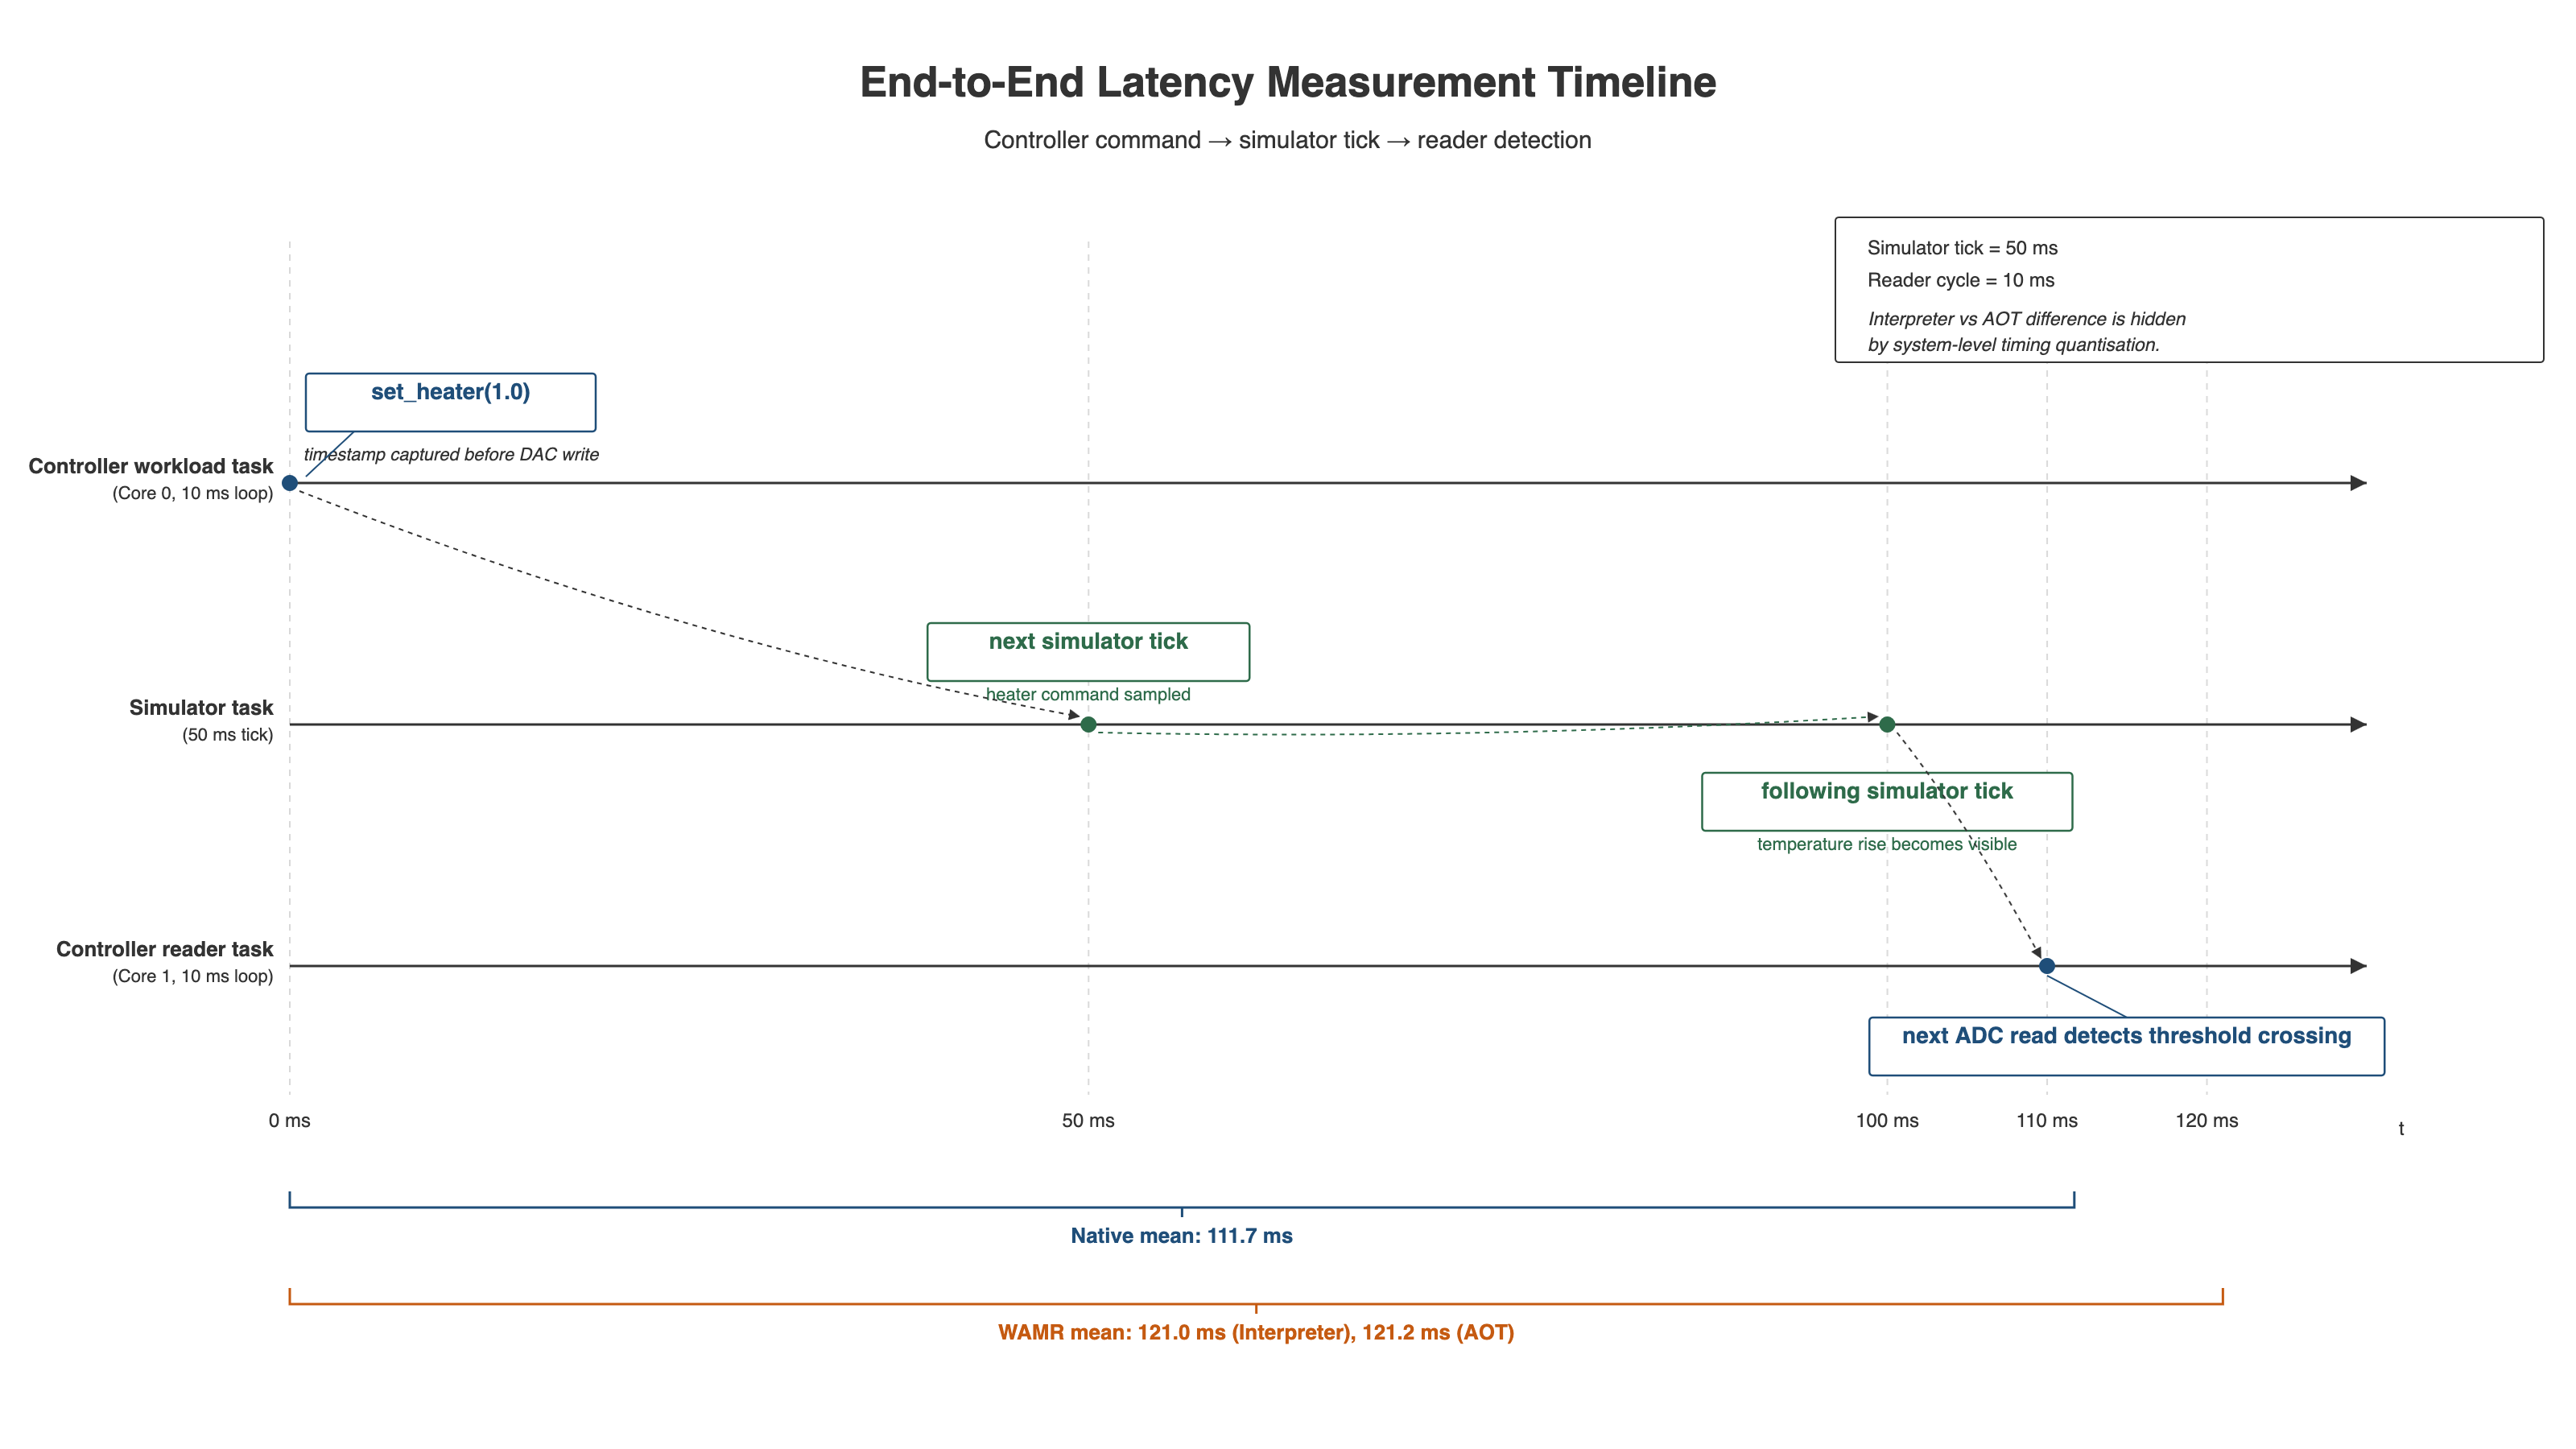
\includegraphics[width=0.95\textwidth]{images/e2e_timing_timeline.png}
    \caption{Discrete-time timeline for the end-to-end latency measurement.}
    \label{fig:e2e-timing-timeline}
\end{figure}

\subsection{Experimental setup}
\label{sec:perf-setup}

All performance profiling experiments were conducted on the two-board testbed described in Chapter~\ref{ch:design}. The Controller board was reflashed between runs with one of three firmware variants: native, WAMR interpreter, or WAMR AOT. The Simulator board ran the same firmware throughout so that only the controller execution environment changed between runs. The experiments used ESP-IDF v5.4, WAMR as an ESP-IDF managed component, and Wasm containers compiled with \texttt{wasi-sdk} 25.0 using \texttt{-O3} optimisation.

Each firmware variant was evaluated using the bang-bang controller, the PID controller, and the step-response workload, giving nine runs in total. The bang-bang and PID workloads ran for 1000 iterations at a 100~ms control period. The step-response workload ran for 9500 iterations at a 10~ms period, which allowed it to capture six end-to-end latency events over the full experiment. Before each run, the simulator was reset to ambient using the GPIO reset signal. The CSV capture covered all timing samples for the bang-bang and PID runs; for the longer step-response run, the fixed-size metrics buffer retained the final 1000 timing samples alongside all six end-to-end events. The serial capture pipeline used a timeout of 130~s for bang-bang and PID runs and 150~s for step-response runs.

\subsection{Data capture pipeline}
\label{subsec:data-pipeline}

A Python script (\texttt{exec\_esp32.py}) automates the flash-and-capture workflow. It flashes the firmware to the ESP32, opens the serial port, and captures output until the \texttt{<<<CSV\_END>>>} marker is detected. The script extracts the CSV block and writes it to a \texttt{results.csv} file. A second script (\texttt{compare\_stats.py}) loads the native and WAMR CSV files, computes per-metric summary statistics (mean, standard deviation, min, max), and produces a side-by-side comparison table with ratios. This pipeline ensures that results are reproducible across runs and that the same statistical analysis is applied consistently to both controller variants.

\section{Metrics}
\label{sec:perf-metrics}

\subsection{Timing and resource metrics}
\label{subsec:metric-defs}

All execution variants collect identical metrics at each control loop iteration and output them in a common CSV format. Table~\ref{tab:metrics} defines each metric.

\begin{table}[ht]
\centering
\small
\begin{tabular}{@{}llp{7.5cm}@{}}
\toprule
\textbf{Metric} & \textbf{Unit} & \textbf{Description} \\
\midrule
\texttt{exec\_time\_us} & \textmu{}s & Total wall-clock execution time of the algorithm (single value per run). \\
\texttt{loop\_time\_us} & \textmu{}s & Time between consecutive delay calls; one full control loop iteration. \\
\texttt{adc\_time\_us} & \textmu{}s & Full ADC read cycle in \texttt{reader\_task}, including calibration and mutex operations. \\
\texttt{heater\_time\_us} & \textmu{}s & Time for a single heater write, including DAC output and E2E arming. \\
\texttt{temp\_get\_time\_us} & \textmu{}s & Time for a single temperature read from the shared variable under mutex. \\
\texttt{e2e\_time\_us} & \textmu{}s & End-to-end signal propagation delay from heater command to threshold crossing. \\
\texttt{free\_heap} & bytes & Available heap memory at each ADC read. \\
\texttt{cpu\_core0} & \% & Core~0 CPU utilisation. \\
\texttt{cpu\_core1} & \% & Core~1 CPU utilisation. \\
\texttt{temp\_mutex\_wait} & \textmu{}s & Time spent by \texttt{reader\_task} acquiring \texttt{temp\_mutex}. \\
\texttt{metrics\_mutex\_wait} & \textmu{}s & Time spent by  \texttt{reader\_task} acquiring \texttt{metrics\_mutex}. \\
\bottomrule
\end{tabular}
\caption{Metrics collected by all execution variants.}
\label{tab:metrics}
\end{table}

All timing measurements use \texttt{esp\_timer\_get\_time()}, which returns a 64-bit microsecond timestamp from a hardware timer. The buffer depth of 1000 captures all iterations for bang-bang and PID runs, and the final 1000 samples for the step-response algorithm, providing complete coverage of both transient and steady-state behaviour.

\subsection{Host-function metrics}
\label{subsec:host-function-overhead}

The seven core host functions described in Section~\ref{subsec:host-functions-design} are the sole interface between the Wasm control algorithms and the physical hardware. From a performance perspective, the critical observation is that \texttt{host\_get\_temperature} and \texttt{host\_set\_heater} are called on every control loop iteration, making their boundary-crossing overhead a per-iteration fixed cost. The timing and recording host functions (\texttt{host\_get\_time\_us}, \texttt{host\_record\_heater\_time}, \texttt{host\_record\_temp\_get\_time}) allow the Wasm module to measure the duration of these calls from within the Wasm execution context, capturing the full overhead including argument marshalling, signature validation, and operand stack transitions that would be invisible if timing were performed only on the native side. The measured overhead for each host function is reported in Section~\ref{sec:host-overhead}.

\section{Results}
\label{sec:perf-results}

The results are organised from functional behaviour to lower-level cost. We first verify that the native, interpreter, and AOT variants produce the same control behaviour on the simulated plant. The timing and host-function measurements then isolate the runtime overhead introduced by the Wasm boundary, while the memory, CPU, and end-to-end latency measurements show how that overhead appears at system level.

\subsection{Control behaviour}
\label{sec:algo-temp-response}

This section first checks the plant-level behaviour of the three execution variants. That comparison matters because the later timing analysis is only meaningful if native and Wasm are solving the same control problem and producing the same thermal response. All three algorithms target 40\textdegree C and run for 1000 iterations at a 100~ms control period (total runtime $\approx$100~s), except the step-response workload, which uses a 10~ms period across 9500 iterations (95~s). The simulator is reset to ambient (25\textdegree C) before each run.

\subsubsection{Bang-bang controller}
\label{subsec:bb-response}

The bang-bang controller exhibits the characteristic limit-cycle oscillation of hysteresis control. Starting from ambient, the native variant reaches the target band within approximately 12 iterations (1.2~s), then oscillates between approximately 38.5\textdegree C and 42.7\textdegree C with a period of $\approx$2.9~s. The amplitude exceeds the $\pm$1\textdegree C hysteresis band because the simulator's thermal inertia and 50~ms tick rate cause overshoot before the heater state change takes effect.

\begin{figure}[htbp]
    \centering
    \begin{subfigure}[t]{0.32\textwidth}
        \centering
        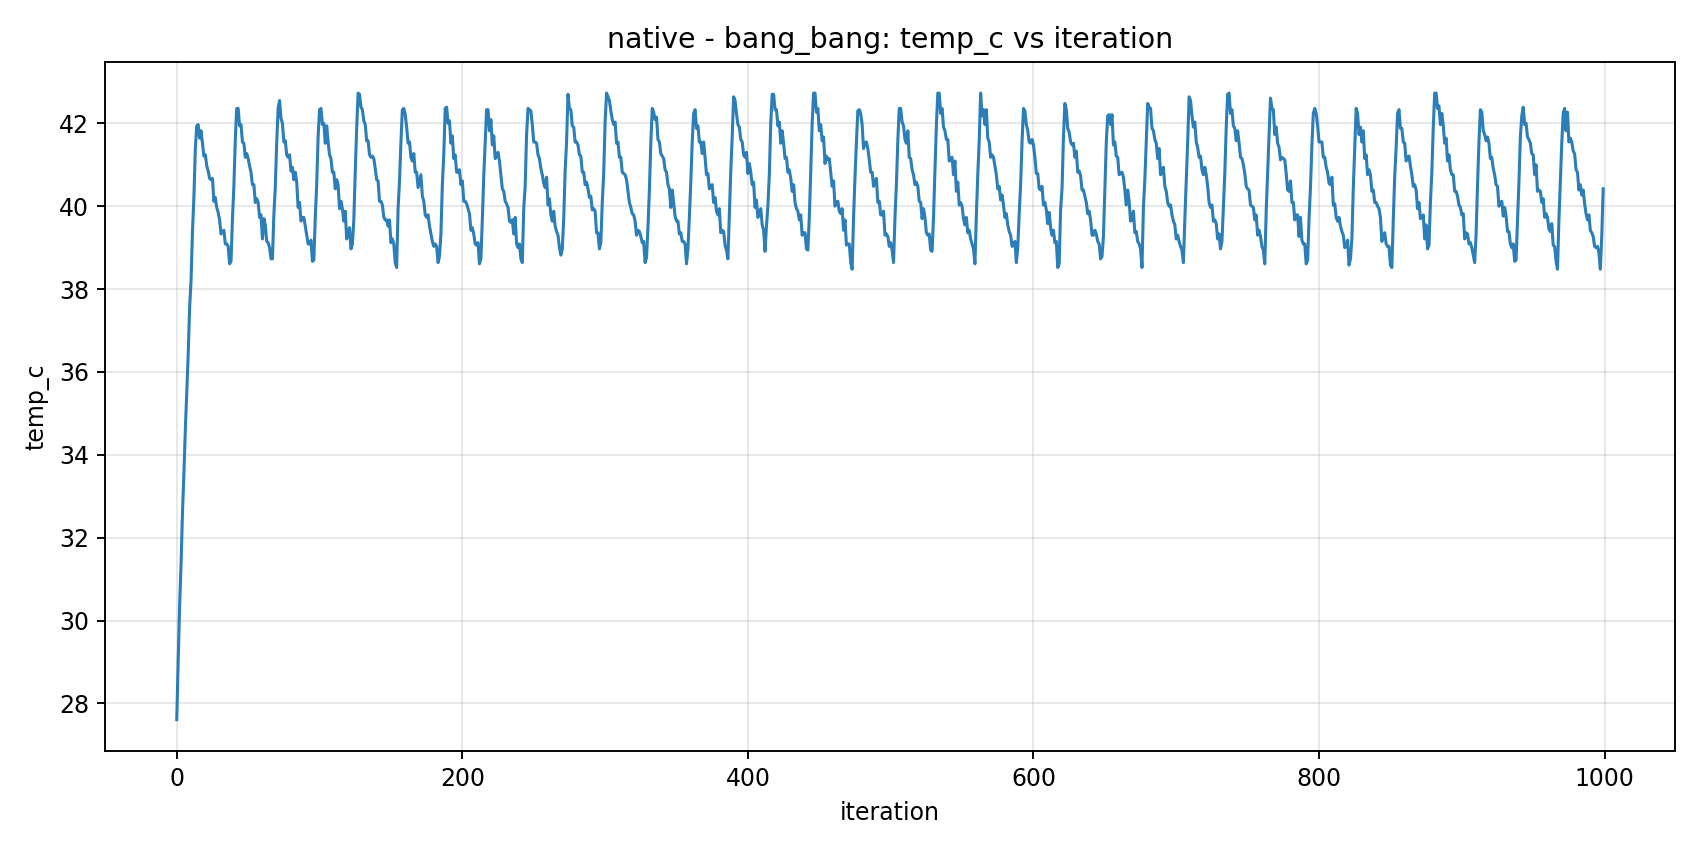
\includegraphics[width=\textwidth]{images/native_bang_bang_temp_vs_iteration.png}
        \caption{Native}
        \label{fig:bb-temp-native}
    \end{subfigure}
    \hfill
    \begin{subfigure}[t]{0.32\textwidth}
        \centering
        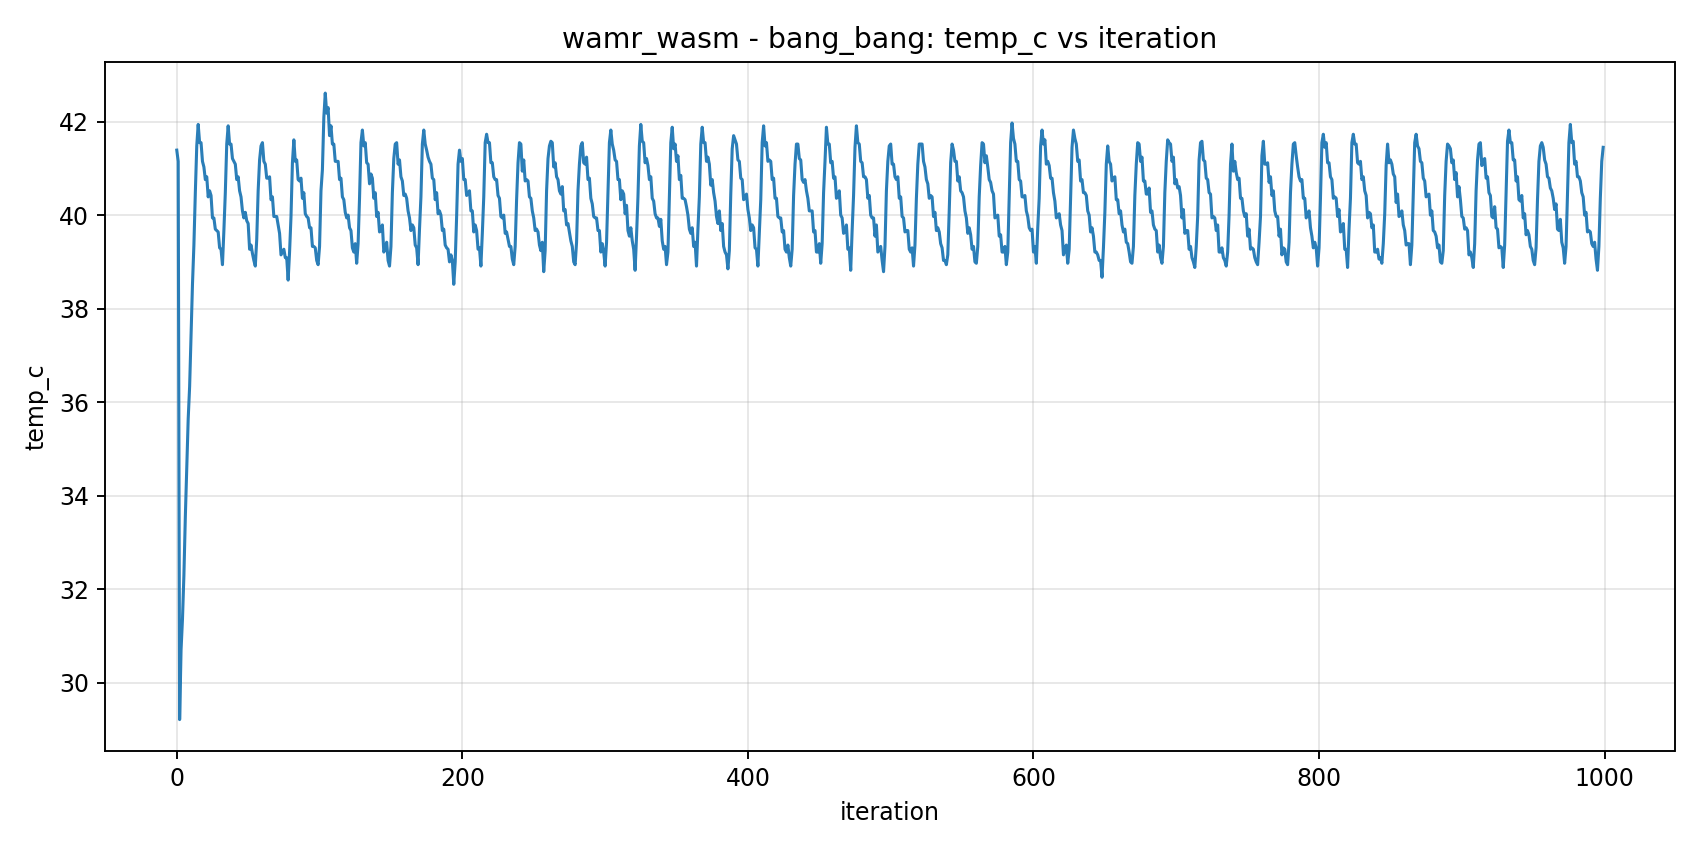
\includegraphics[width=\textwidth]{images/wamr_wasm_bang_bang_temp_vs_iteration.png}
        \caption{Interpreter}
        \label{fig:bb-temp-interpreter}
    \end{subfigure}
    \hfill
    \begin{subfigure}[t]{0.32\textwidth}
        \centering
        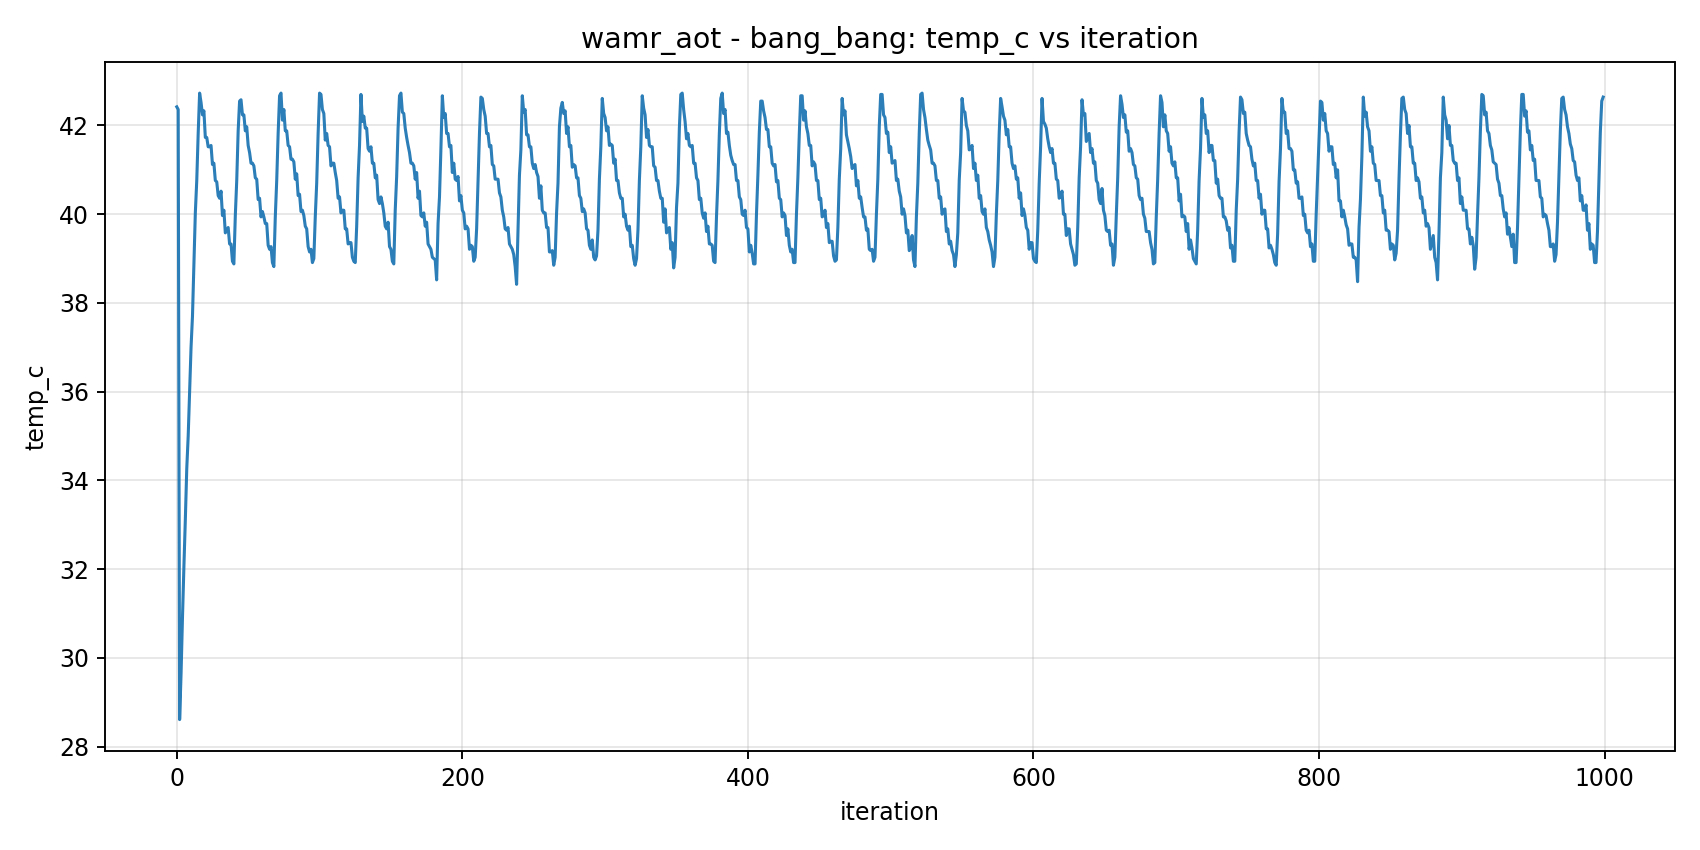
\includegraphics[width=\textwidth]{images/wamr_aot_bang_bang_temp_vs_iteration.png}
        \caption{AOT}
        \label{fig:bb-temp-aot}
    \end{subfigure}
    \caption{Bang-bang controller temperature response across execution variants.}
    \label{fig:bb-temp}
\end{figure}

Figure~\ref{fig:bb-temp} shows that the WAMR interpreter and AOT variants produce the same behaviour in practice. Their steady-state means all remain within 0.6\textdegree C of the 40\textdegree C setpoint, and their oscillation periods and waveform shapes are effectively the same. This indicates that runtime overhead appears in the timing metrics rather than as degraded bang-bang control behaviour.

\subsubsection{PID controller}
\label{subsec:pid-response}


The PID controller ($K_p = 1.2$, $K_i = 0.08$, $K_d = 0.25$) produces a smoother response than bang-bang control. From ambient, the native variant reaches the 40\textdegree C target within approximately 13 iterations (1.3~s), overshoots to $\approx$42.0\textdegree C, and then settles around the setpoint. Its steady-state variation is driven mainly by the simulator's $\pm$0.3\textdegree C sensor noise and the proportional and derivative terms.

\begin{figure}[htbp]
    \centering
    \begin{subfigure}[t]{0.32\textwidth}
        \centering
        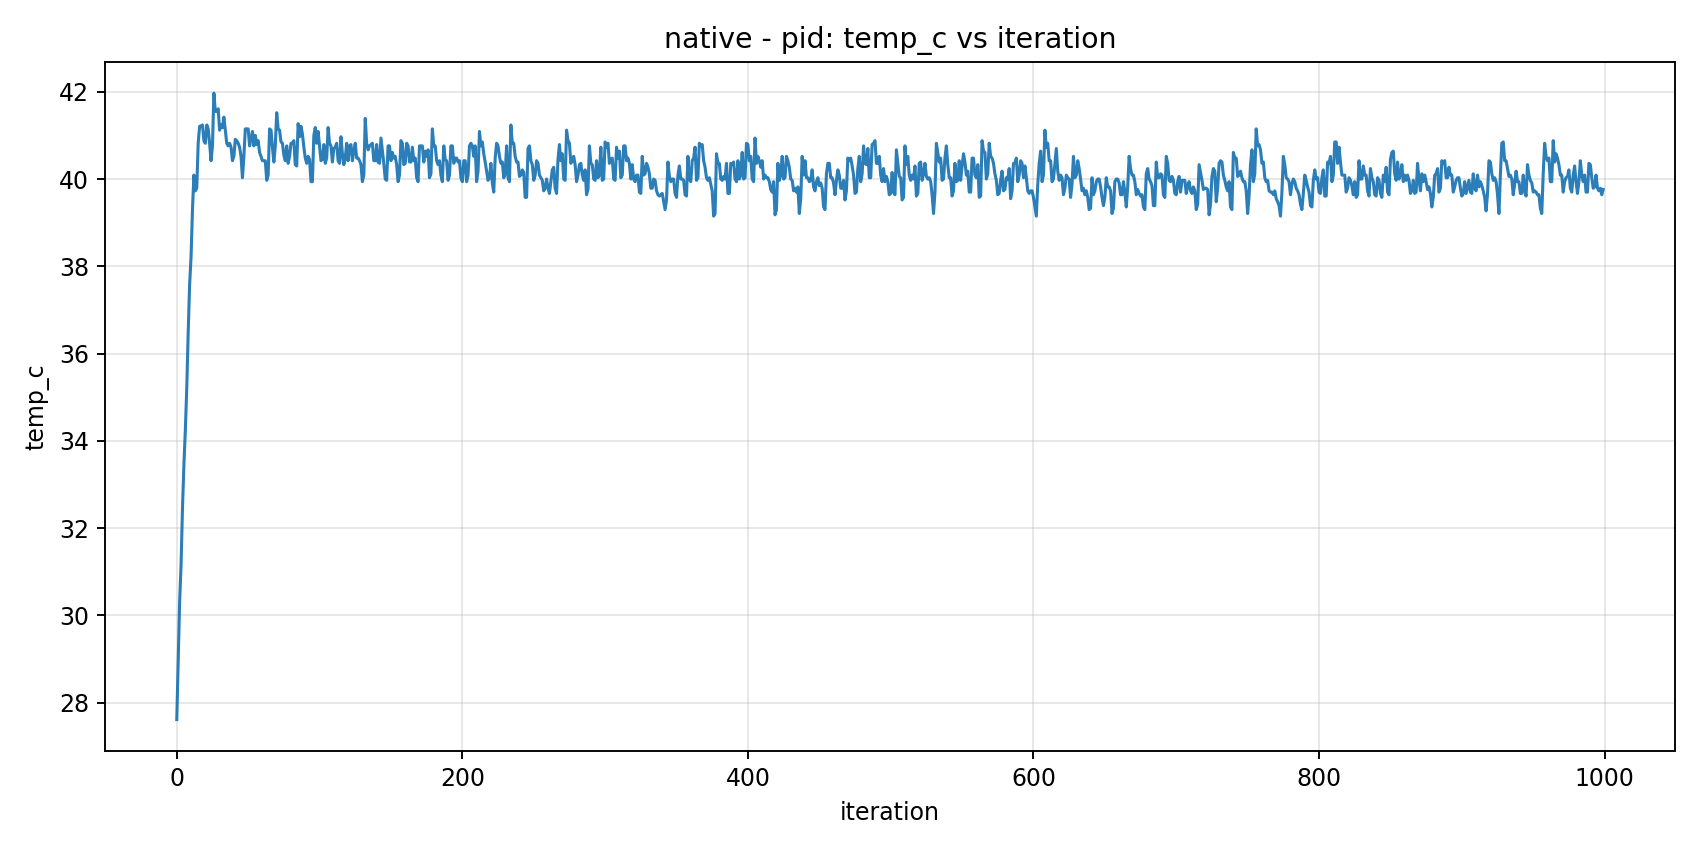
\includegraphics[width=\textwidth]{images/native_pid_temp_vs_iteration.png}
        \caption{Native}
        \label{fig:pid-temp-native}
    \end{subfigure}
    \hfill
    \begin{subfigure}[t]{0.32\textwidth}
        \centering
        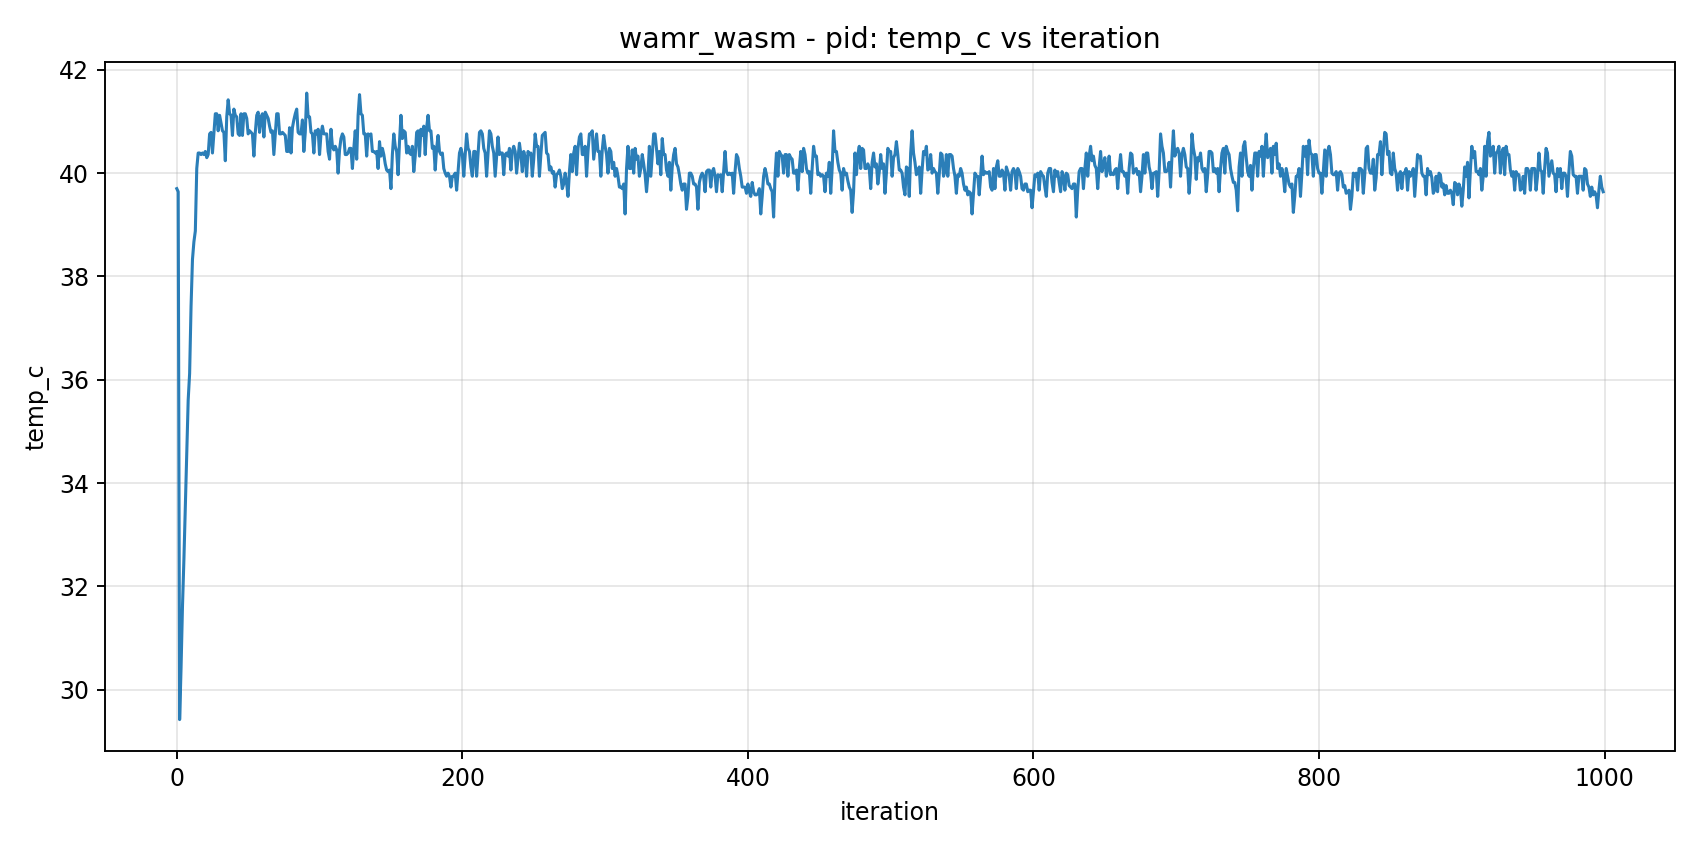
\includegraphics[width=\textwidth]{images/wamr_wasm_pid_temp_vs_iteration.png}
        \caption{Interpreter}
        \label{fig:pid-temp-interpreter}
    \end{subfigure}
    \hfill
    \begin{subfigure}[t]{0.32\textwidth}
        \centering
        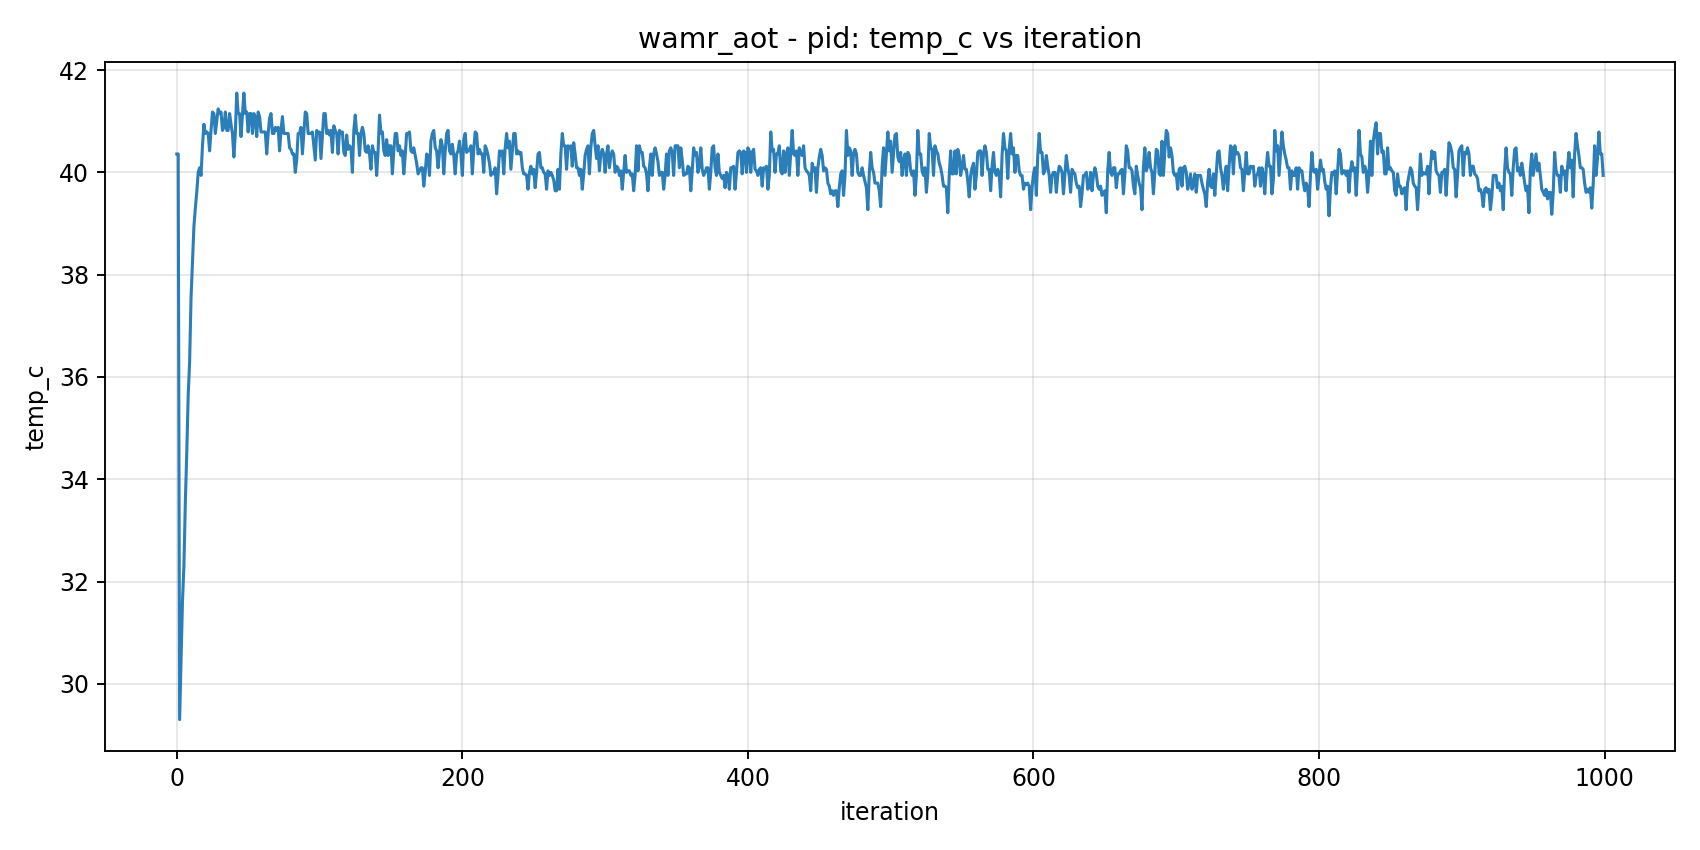
\includegraphics[width=\textwidth]{images/wamr_aot_pid_temp_vs_iteration.png}
        \caption{AOT}
        \label{fig:pid-temp-aot}
    \end{subfigure}
    \caption{PID controller temperature response across execution variants.}
    \label{fig:pid-temp}
\end{figure}

Figure~\ref{fig:pid-temp} shows consistent steady-state performance across all three execution variants. Their final mean temperatures are all 39.99\textdegree C, with similar standard deviations and settling times. This shows that the Wasm runtime does not degrade the PID controller's ability to maintain the setpoint within this workload.

\subsubsection{Step-response algorithm}
\label{subsec:e2e-response}

The step-response algorithm is a diagnostic workload rather than a closed-loop controller. After a 5-second stabilisation period, it performs six heating cycles: 3~seconds at full heater power followed by 12~seconds of cooldown. This produces independent temperature rises for measuring end-to-end signal propagation latency. Figure~\ref{fig:e2e-timing-timeline} shows a visual timeline for this algorithm.

\begin{figure}[htbp]
    \centering
    \begin{subfigure}[t]{0.32\textwidth}
        \centering
        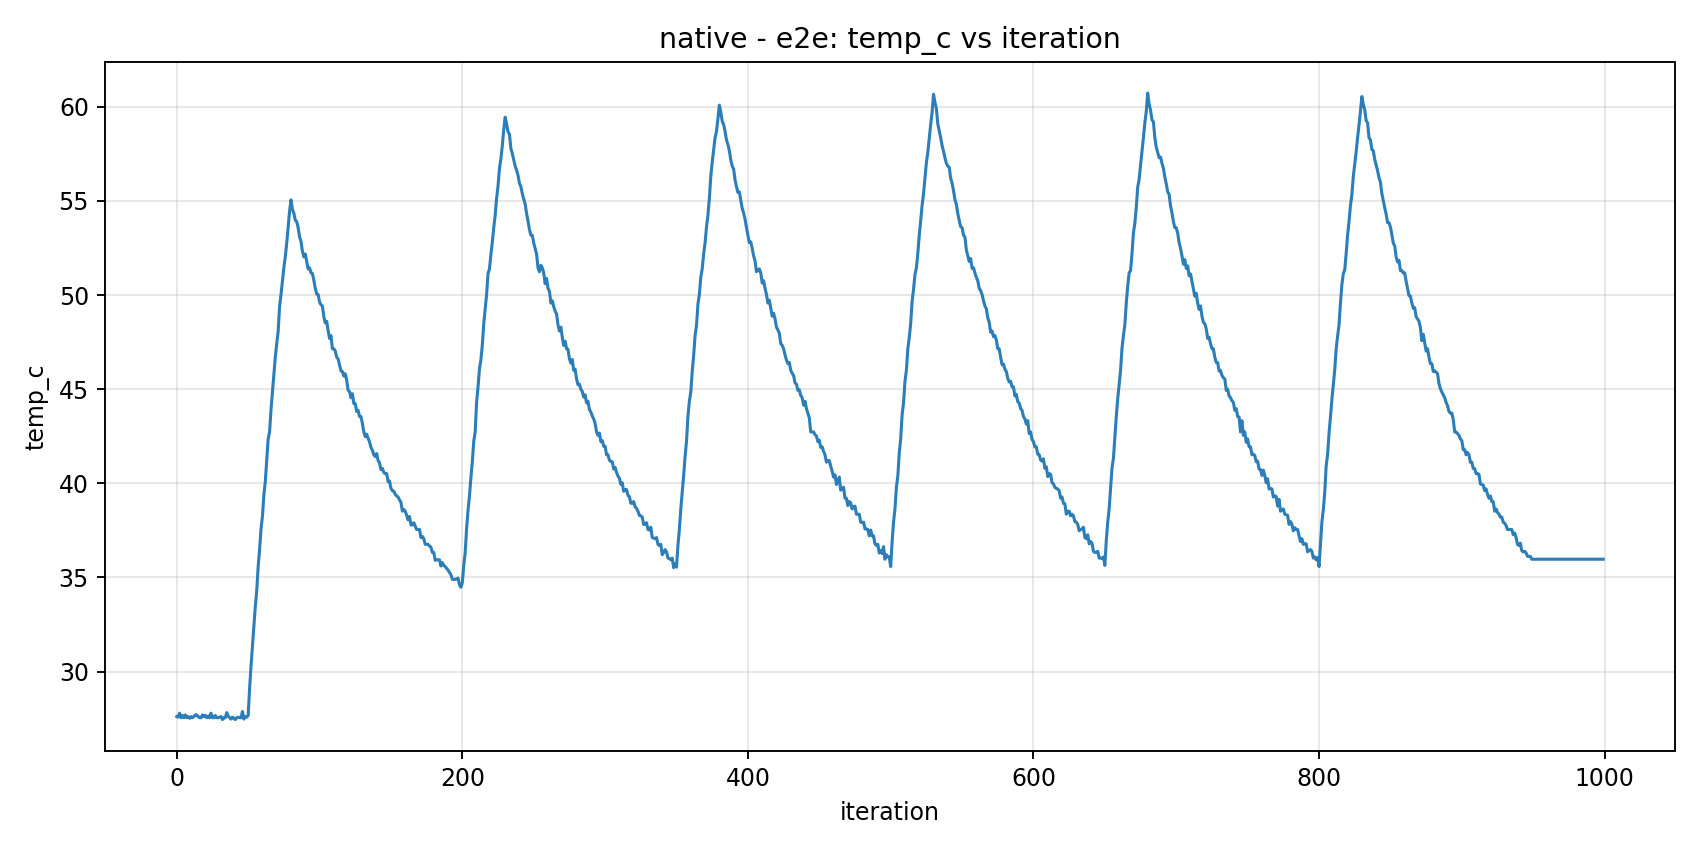
\includegraphics[width=\textwidth]{images/native_e2e_temp_vs_iteration.png}
        \caption{Native}
        \label{fig:e2e-temp-native}
    \end{subfigure}
    \hfill
    \begin{subfigure}[t]{0.32\textwidth}
        \centering
        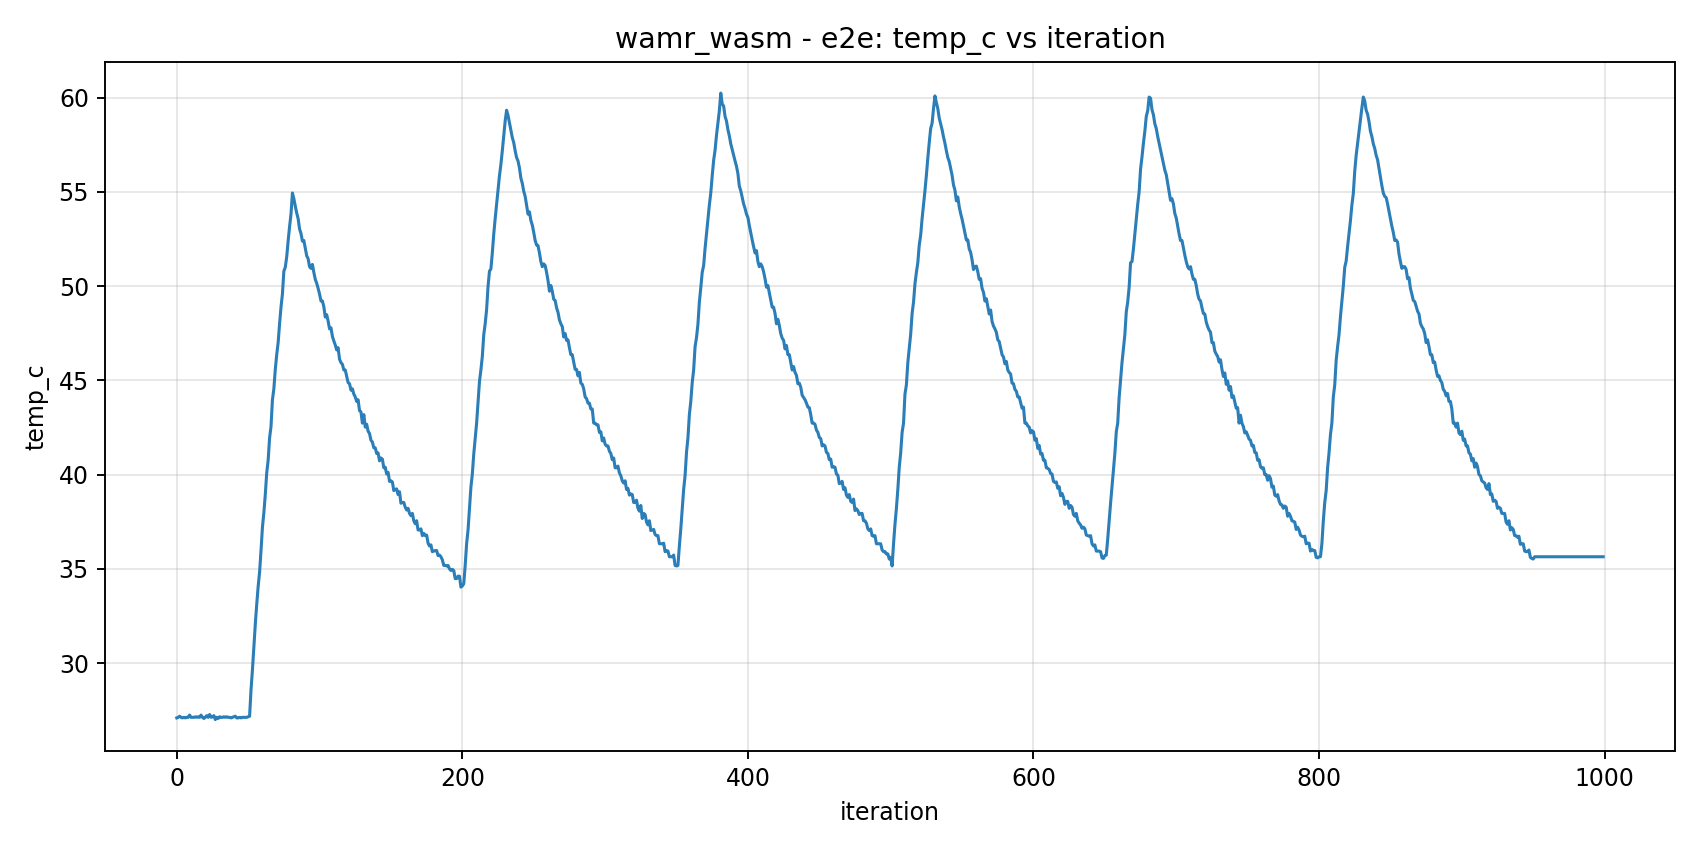
\includegraphics[width=\textwidth]{images/wamr_wasm_e2e_temp_vs_iteration.png}
        \caption{Interpreter}
        \label{fig:e2e-temp-interpreter}
    \end{subfigure}
    \hfill
    \begin{subfigure}[t]{0.32\textwidth}
        \centering
        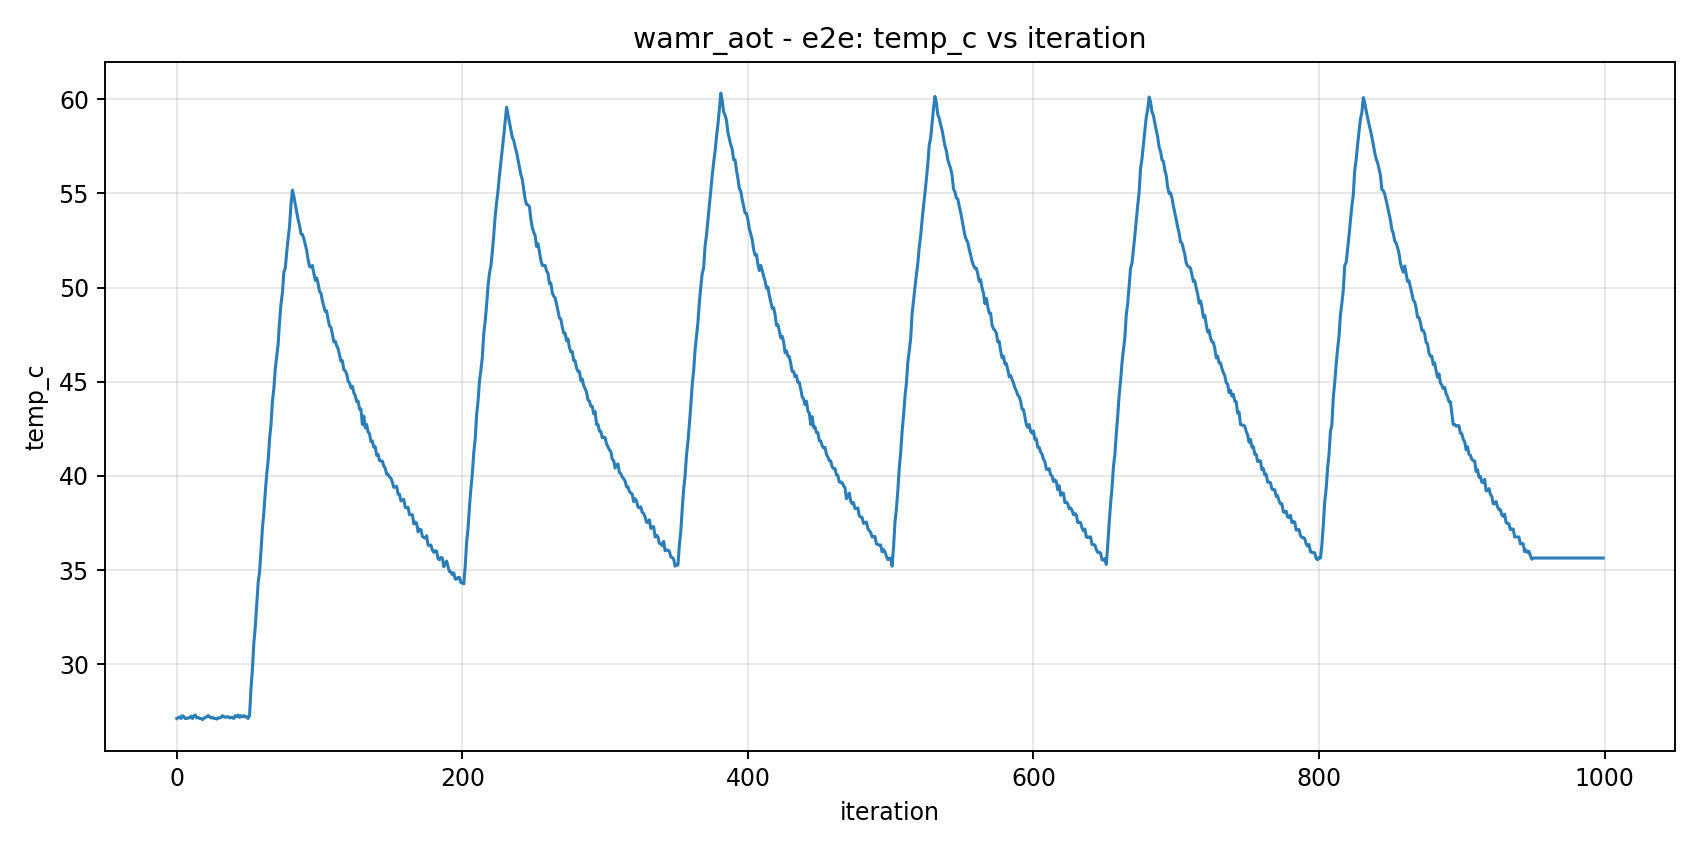
\includegraphics[width=\textwidth]{images/wamr_aot_e2e_temp_vs_iteration.png}
        \caption{AOT}
        \label{fig:e2e-temp-aot}
    \end{subfigure}
    \caption{Step-response temperature profile across execution variants.}
    \label{fig:e2e-temp}
\end{figure}

Figure~\ref{fig:e2e-temp} shows six sawtooth-like cycles for each execution variant, with peak temperatures remaining consistent across native, interpreter, and AOT runs. The workload is therefore comparable across variants. The E2E latency means differ, however: native averages 111.7~ms, while interpreter and AOT average 121.0~ms and 121.2~ms respectively. This latency gap is analysed later as a system-level effect of runtime overhead and discrete simulator timing.

\subsubsection{Cross-variant comparison}
\label{subsec:temp-comparison}

Table~\ref{tab:temp-response} summarises the temperature control characteristics across all variants and algorithms.

\begin{table}[htbp]
\centering
\caption{Temperature response characteristics across execution variants. All algorithms target 40\textdegree C.}
\label{tab:temp-response}
\small
\begin{tabular}{@{}llccc@{}}
\toprule
\textbf{Algorithm} & \textbf{Metric} & \textbf{Native} & \textbf{Interpreter} & \textbf{AOT} \\
\midrule
\multirow{3}{*}{Bang-bang}
    & Steady-state mean (\textdegree C) & 40.46 & 40.22 & 40.59 \\
    & Oscillation range (\textdegree C) & 38.5--42.7 & 38.7--42.0 & 38.5--42.7 \\
    & Oscillation period (s) & $\approx$2.9 & $\approx$2.9 & $\approx$2.9 \\
\midrule
\multirow{3}{*}{PID}
    & Steady-state mean (\textdegree C) & 39.99 & 39.99 & 39.99 \\
    & Steady-state $\sigma$ (\textdegree C) & 0.32 & 0.30 & 0.35 \\
    & Initial overshoot (\textdegree C) & 1.97 & 1.55 & 1.55 \\
\midrule
\multirow{2}{*}{Step-response}
    & Peak temperature (\textdegree C) & 60.7 & 60.2 & 60.3 \\
    & E2E latency mean (ms) & 111.7 & 121.0 & 121.2 \\
\bottomrule
\end{tabular}
\end{table}

The central finding is that the WebAssembly runtime---whether in interpreter or AOT mode---does not measurably degrade the temperature control quality of any algorithm at a 100~ms control period. The steady-state means, oscillation amplitudes, and settling times are statistically indistinguishable across variants. This is expected: at 100~ms per iteration, even the interpreter's per-loop overhead (on the order of hundreds of microseconds, as detailed in Section~\ref{sec:host-overhead}) constitutes less than 1\% of the control period, leaving the timing budget overwhelmingly dominated by the \texttt{vTaskDelay()} call. The performance differences between variants become visible only in the fine-grained timing metrics examined in the following sections.

\subsection{Execution time overhead}
\label{sec:exec-time}

The total wall-clock execution time (\texttt{exec\_time\_us}) measures the complete algorithm lifecycle: from runtime initialisation (for WAMR) or task entry (for native) through all control loop iterations to completion. Table~\ref{tab:exec-time} presents the results across all three algorithms.

\begin{table}[htbp]
\centering
\caption{Total execution time (seconds) by algorithm and execution variant.}
\label{tab:exec-time}
\small
\begin{tabular}{@{}lccc@{}}
\toprule
\textbf{Algorithm} & \textbf{Native} & \textbf{Interpreter} & \textbf{AOT} \\
\midrule
Bang-bang (1000 $\times$ 100\,ms) & 100.00 & 100.17 (+0.17\%) & 100.17 (+0.17\%) \\
PID (1000 $\times$ 100\,ms) & 100.00 & 100.16 (+0.16\%) & 100.17 (+0.17\%) \\
Step-response (9500 $\times$ 10\,ms) & 95.00 & 95.17 (+0.18\%) & 95.18 (+0.18\%) \\
\bottomrule
\end{tabular}
\end{table}

The overhead is remarkably small: less than 0.2\% for both WAMR execution modes across all algorithms. This is because the total runtime is dominated by \texttt{vTaskDelay()} calls within each iteration. For bang-bang and PID, the 1000 iterations at 100~ms account for 100~s of wall-clock time, during which the processor is yielded to the RTOS scheduler. The actual computation per iteration (sensor read, algorithm, actuator write) completes in under 1~ms, meaning the per-iteration Wasm overhead of tens to hundreds of microseconds is amortised across the 100~ms delay period. The $\approx$170~ms total overhead for WAMR runs is consistent with the one-time WAMR initialisation cost (SPIFFS mount, runtime init, module load, instantiation) rather than accumulated per-iteration overhead.

Notably, interpreter and AOT exhibit nearly identical total execution times. This confirms that at a 100~ms control period, the per-iteration overhead difference between interpreter and AOT (examined in detail in Section~\ref{sec:host-overhead}) is too small relative to the delay period to produce a measurable difference in wall-clock time.

\subsection{Loop timing and jitter}
\label{sec:loop-timing}

The \texttt{loop\_time\_us} metric measures the actual time between consecutive \texttt{vTaskDelay()} calls---effectively the real control period as experienced by the plant. Deviation from the configured period constitutes \textit{jitter}, which can degrade control stability if it becomes a significant fraction of the control period.

\begin{table}[htbp]
\centering
\caption{Loop timing statistics (\textmu{}s) for the PID algorithm (configured period: 100,000\,\textmu{}s).}
\label{tab:loop-timing}
\small
\begin{tabular}{@{}lcccc@{}}
\toprule
\textbf{Variant} & \textbf{Mean} & \textbf{Std Dev} & \textbf{Min} & \textbf{Max} \\
\midrule
Native       & 99,999.7 & 181.8 & 99,574 & 100,425 \\
Interpreter  & 99,999.7 & 7.8   & 99,794 & 100,006 \\
AOT          & 99,999.7 & 7.3   & 99,770 & 100,001 \\
\bottomrule
\end{tabular}
\end{table}

Table~\ref{tab:loop-timing} presents the PID results, which are representative of the 100~ms steady-state workloads. PID is used here because it exercises the same periodic sensing and actuation structure as bang-bang while avoiding the deadband-dependent skipped writes that make bang-bang timing less uniform. All three variants achieve the target 100~ms period with sub-millisecond accuracy. The mean loop time is effectively identical across variants.

Counter-intuitively, the WAMR variants exhibit \textit{lower} jitter than native ($\sigma = 7$--8~\textmu{}s vs.\ 182~\textmu{}s). This is explained by how each variant enters the delay. The native controller calls \texttt{vTaskDelay()} directly, and the FreeRTOS tick granularity (1~ms by default) introduces rounding that varies depending on where within a tick the delay is requested. The WAMR variants call \texttt{host\_delay()}, which passes through the host function dispatch before reaching \texttt{vTaskDelay()}. The additional constant overhead of the host function call shifts the delay request to a more consistent position within the tick cycle, effectively acting as a timing synchroniser. The step-response algorithm (10~ms period) shows higher jitter for all variants ($\sigma \approx 190$--370~\textmu{}s), as the shorter period makes the 1~ms tick granularity a proportionally larger source of variation.

For control-theoretic purposes, the worst-case jitter of $\pm$450~\textmu{}s at a 100~ms period represents 0.45\% of the control period---well within the acceptable range for thermal control, where the plant dynamics operate on timescales of seconds.

\subsection{Host-function call overhead}
\label{sec:host-overhead}

The host function call overhead is the per-call cost of crossing the Wasm--native boundary. It is the most direct measure of the runtime's execution penalty, isolated from the control period and delay timing. Two host functions are called on every control iteration: \texttt{host\_get\_temperature} (sensor read) and \texttt{host\_set\_heater} (actuator write). Their timings are recorded from within the Wasm module using \texttt{host\_get\_time\_us}, capturing the full round-trip including argument marshalling, signature validation, native function dispatch, and return value propagation.

\subsubsection{Temperature read overhead}
\label{subsec:temp-get-overhead}

\texttt{host\_get\_temperature} acquires a mutex, reads a float variable, and returns it. The native equivalent performs the same operations without a boundary crossing.

\begin{table}[htbp]
\centering
\label{tab:temp-get}
\small
\begin{tabular}{@{}lcccc@{}}
    \toprule
    \textbf{Variant} & \textbf{Mean} & \textbf{p50} & \textbf{p99} & \textbf{Overhead vs.\ Native} \\
    \midrule
    Native       & 8.2  & 8  & 10 & --- \\
    Interpreter  & 67.0 & 67 & 67 & 8.2$\times$ (+59~\textmu{}s) \\
    AOT          & 31.0 & 31 & 31 & 3.8$\times$ (+23~\textmu{}s) \\
    \bottomrule
\end{tabular}
\caption{\texttt{temp\_get\_time\_us} (\textmu{}s) across algorithms and variants. The PID values are representative of steady-state behaviour.}
\end{table}

The interpreter adds 59~\textmu{}s per temperature read, while AOT adds 23~\textmu{}s. These values are remarkably consistent across algorithms: the standard deviation is below 1~\textmu{}s for both WAMR modes, and the p50 and p99 values are identical, indicating that the overhead is a deterministic fixed cost with no tail latency. The consistency across bang-bang (mean 67.1~\textmu{}s), PID (67.0~\textmu{}s), and step-response (71.7~\textmu{}s) for the interpreter confirms that the overhead is independent of the calling algorithm's complexity.

\subsubsection{Heater write overhead}
\label{subsec:heater-overhead}

\texttt{host\_set\_heater} is more complex: it clamps the input, writes the DAC, reads the current temperature under mutex for E2E baselining, records the timestamp, and arms the E2E trigger. The PID algorithm calls \texttt{set\_heater} on every iteration with a continuously varying command, making it the cleanest benchmark for this function.

\begin{table}[htbp]
\centering
\caption{\texttt{heater\_time\_us} (\textmu{}s) for the PID algorithm.}
\label{tab:heater-time}
\small
\begin{tabular}{@{}lcccc@{}}
\toprule
\textbf{Variant} & \textbf{Mean} & \textbf{p50} & \textbf{p99} & \textbf{Overhead vs.\ Native} \\
\midrule
Native       & 20.2  & 20  & 21  & --- \\
Interpreter  & 132.9 & 134 & 135 & 6.6$\times$ (+113~\textmu{}s) \\
AOT          & 45.3  & 45  & 46  & 2.2$\times$ (+25~\textmu{}s) \\
\bottomrule
\end{tabular}
\end{table}

The absolute overhead is larger than for temperature reads because the underlying native function performs more work (DAC write, mutex acquisition, timestamp recording). However, the \textit{boundary-crossing} overhead---the difference attributable to Wasm rather than to the native function body---can be estimated by subtracting the native baseline: 113~\textmu{}s for interpreter and 25~\textmu{}s for AOT. These values are consistent with the 59~\textmu{}s and 23~\textmu{}s measured for the simpler temperature read, suggesting that the interpreter's per-call boundary cost is approximately 60--110~\textmu{}s while AOT's is approximately 23--25~\textmu{}s.

The bang-bang controller exhibits bimodal heater timing because approximately 57\% of iterations fall within the hysteresis deadband, where the heater state does not change and the DAC write is skipped, producing heater times of 1--2~\textmu{}s (native) or 34--40~\textmu{}s (interpreter). The remaining 43\% of iterations trigger a DAC write and produce times consistent with the PID measurements. This bimodality does not affect the overhead analysis but explains the higher variance in bang-bang heater timing ($\sigma = 10.9$~\textmu{}s native, $35.5$~\textmu{}s interpreter) compared to PID ($\sigma = 3.9$~\textmu{}s native, $5.3$~\textmu{}s interpreter).

\subsubsection{Overhead sources}
\label{subsec:overhead-sources}

The interpreter's higher per-call cost originates from WAMR's fast interpreter dispatch loop. When a Wasm module calls an imported function, the interpreter must decode the \texttt{call} instruction from the pre-compiled internal bytecode, look up the native symbol in the registered function table, validate the function signature, marshal arguments from the Wasm operand stack to the native C calling convention, invoke the native function through a function pointer, and marshal the return value back onto the operand stack. Each of these steps adds memory indirections and branches before the native work even begins.

AOT-compiled code removes the bytecode decode and dispatch stages entirely. The \texttt{wamrc} compiler resolves import calls ahead of time, generating direct native call instructions with inline argument marshalling. The remaining 23--25~\textmu{}s overhead reflects the residual cost of the WAMR ABI wrapper: saving and restoring the execution environment context, validating linear-memory bounds, and performing the indirect call through the relocation table.

\subsubsection{Per-iteration budget}
\label{subsec:per-iter-budget}

Each control iteration makes two host function calls (one temperature read, one heater write). The total per-iteration Wasm overhead is therefore approximately 170~\textmu{}s for the interpreter and 48~\textmu{}s for AOT. At a 100~ms control period, this represents 0.17\% (interpreter) and 0.05\% (AOT) of the available time budget---negligible for thermal control. At a 10~ms period (step-response), the overhead rises to 1.7\% (interpreter) and 0.48\% (AOT), still well within the budget. The overhead would only become problematic at control periods below approximately 1~ms, where the interpreter's 170~\textmu{}s per iteration would consume 17\% of the available budget.

\subsection{Memory footprint}
\label{sec:memory}

The \texttt{free\_heap} metric reports the available heap memory on the ESP32 during algorithm execution. Since both firmware variants allocate identical support task stacks, metrics buffers, and driver structures, the difference in free heap between native and WAMR directly reflects the memory consumed by the Wasm runtime.

\begin{table}[htbp]
\centering
\caption{Free heap (bytes) during steady-state algorithm execution. Values are constant within each run.}
\label{tab:free-heap}
\small
\begin{tabular}{@{}lccc@{}}
\toprule
\textbf{Algorithm} & \textbf{Native} & \textbf{Interpreter} & \textbf{AOT} \\
\midrule
Bang-bang      & 210,048 & 133,956 & 129,200 \\
PID            & 210,048 & 133,884 & 128,816 \\
Step-response  & 210,048 & 132,872 & 123,696 \\
\bottomrule
\end{tabular}
\end{table}

The native controller consistently leaves 210~KB of free heap across all algorithms. The WAMR interpreter consumes an additional $\approx$76~KB (reducing free heap to $\approx$134~KB), and AOT consumes $\approx$81--86~KB (reducing free heap to $\approx$124--129~KB). On an ESP32 with 520~KB of total SRAM, the WAMR runtime overhead represents 15--17\% of total memory.

\subsubsection{Memory breakdown}
\label{subsec:memory-breakdown}

The $\approx$76--86~KB consumed by WAMR is distributed across several categories, as described in Section~\ref{subsec:wamr-memory}:

AOT mode uses slightly more memory than the interpreter between 5-9~KB because the AOT loader must hold the compiled native code in memory alongside the relocation metadata. In interpreter mode, the equivalent space is occupied by the pre-compiled fast interpreter bytecode buffer, which is somewhat smaller than the AOT native code for these simple algorithms.

The minor variation across algorithms reflects differences in the Wasm module's static data size and the number of global variables, which affect the linear memory initialisation. The step-response algorithm declares more configuration constants, resulting in a marginally larger data segment.

\subsubsection{Practical implications}
\label{subsec:memory-implications}

The $\approx$76--86~KB overhead leaves 124--134~KB of free heap on the ESP32, which is sufficient for the current single-module deployment but becomes a constraint for more complex scenarios. Multi-module deployments (as explored in Chapter~\ref{ch:containerization_strategy}) require instantiating additional Wasm modules, each consuming at least 64~KB of linear memory plus stack and metadata. On the ESP32's 520~KB SRAM, this limits practical deployments to two or three concurrent Wasm modules before heap exhaustion. Memory, rather than execution speed, is therefore the primary practical constraint on Wasm adoption for microcontroller-based IoT systems.

\subsection{CPU utilisation}
\label{sec:cpu-utilisation}

CPU utilisation was initially recorded in two ways: through the per-sample CSV columns
\texttt{cpu\_core0}, \texttt{cpu\_core1}, and \texttt{cpu\_overall}, and through the end-of-run
FreeRTOS runtime statistics. The control-algorithm sweep suggested that CPU load depended much
more strongly on execution environment than on the algorithm itself. Native execution kept
Core~1 close to 6.5\% for all three workloads, whereas both WAMR modes reported approximately
15.6--15.8\% on the same core. Core~0 showed the expected increase for the 10~ms step-response
workload, but remained low for the 100~ms bang-bang and PID loops.

\begin{table}[htbp]
\centering
\caption{Mean CPU utilisation (\%) across the control-algorithm sweep.}
\label{tab:cpu-utilisation-summary}
\small
\begin{tabular}{@{}llccc@{}}
\toprule
\textbf{Algorithm} & \textbf{Variant} & \textbf{Core 0} & \textbf{Core 1} & \textbf{Overall} \\
\midrule
Bang-bang & Native      & 0.07 & 6.50 & 3.28 \\
Bang-bang & Interpreter & 1.00 & 15.67 & 8.34 \\
Bang-bang & AOT         & 0.87 & 15.71 & 8.29 \\
\midrule
PID       & Native      & 0.08 & 6.45 & 3.27 \\
PID       & Interpreter & 1.02 & 15.67 & 8.35 \\
PID       & AOT         & 0.89 & 15.71 & 8.30 \\
\midrule
Step-response & Native      & 0.42 & 6.60 & 3.51 \\
Step-response & Interpreter & 2.85 & 15.58 & 9.21 \\
Step-response & AOT         & 1.81 & 15.77 & 8.79 \\
\bottomrule
\end{tabular}
\end{table}

Table~\ref{tab:cpu-utilisation-summary} shows two consistent patterns. First, algorithm choice has
only a minor effect on Core~1 utilisation: within each execution environment, bang-bang, PID, and
step-response all produce very similar Core~1 values. Second, WAMR increases Core~0 usage in the
expected direction, especially for the higher-frequency step-response test, but it also appears to
introduce a large and algorithm-independent Core~1 overhead. 

\subsubsection{Investigation of Core~1 Overhead}
A dedicated CPU-investigation sweep varied both the WAMR execution mode and the core to which the Wasm thread
was pinned. Moving the Wasm thread from Core~0 to Core~1 changed Core~0 utilisation as expected,
but had only a very small effect on Core~1. This indicated that the large Core~1 figure could not
be explained simply by thread placement. A second check increased the CPU-sampler period from
10~ms to 100~ms, but this also left the reported Core~1 utilisation essentially unchanged. The
decisive result came from disabling the CPU-measurement task entirely in the WAMR build. The supporting measurements are provided in Appendix~\ref{app:performance-support}.

The investigation showed that reducing the sampling frequency did not lower
the reported Core~1 load, but removing the measurement task did. Once the sampler was disabled,
the \texttt{CPU Usage} task disappeared from the runtime statistics and Core~1 idle time rose from
84\% to 99\%. The earlier 15--16\% Core~1 figure was therefore dominated by the instrumentation
task itself rather than by an intrinsic background cost of WAMR. Native was not free of this
effect --- its own runtime statistics attribute approximately 6\% of CPU time to the same
measurement task --- but the cost was amplified significantly in the WAMR build.


\subsection{End-to-end signal propagation latency}
\label{sec:e2e-latency}

End-to-end (E2E) latency measures the total time from the controller issuing a heater command to the controller detecting the resulting temperature change. Unlike the per-call host function overhead (Section~\ref{sec:host-overhead}), E2E latency captures the full signal propagation chain: the DAC write on the controller, the analogue signal transit, the simulator's physics update, the DAC output on the simulator, the analogue return path, and the ADC read on the controller. It is the metric most directly relevant to control system responsiveness.

\subsubsection{Measurement methodology}
\label{subsec:e2e-method}

The step-response algorithm (described in Section~\ref{subsec:step-response}) is purpose-built for this measurement. It applies six discrete heating steps, each separated by a 12-second cooldown to ensure thermal independence. At the start of each heating step, \texttt{set\_heater(1.0)} records the current timestamp and baseline temperature under mutex protection, and sets a \texttt{waiting\_for\_rise} flag. The ADC reader task on Core~1 continuously monitors the temperature; when it exceeds the baseline by more than the E2E threshold (0.5\textdegree C), it records the elapsed time as the E2E latency and clears the flag.

The measured latency is governed by a short chain of discrete timing events:

\begin{enumerate}
    \item \textbf{Controller DAC write} ($t_0$): the heater command is written to the DAC and the E2E timer starts.
    \item \textbf{Simulator ADC read} ($t_0 + \Delta_{\text{sim}}$): the simulator reads the heater command on its next 50~ms tick. The wait $\Delta_{\text{sim}}$ is uniformly distributed in $[0, 50]$~ms depending on the phase alignment between the controller's command and the simulator's tick.
    \item \textbf{Physics update}: the simulator computes the new temperature. With the thermal mass ($\alpha = 0.7$) and heating rate (2.0\textdegree C/tick), a single tick at full power raises the temperature by approximately 0.6\textdegree C from a 27\textdegree C baseline---sufficient to cross the 0.5\textdegree C threshold.
    \item \textbf{Simulator DAC output}: the updated temperature is written to the simulator's DAC on the same tick.
    \item \textbf{Controller ADC read} ($t_0 + \Delta_{\text{sim}} + \Delta_{\text{read}}$): the controller's reader task samples the ADC on its next 10~ms cycle and detects the threshold crossing.
\end{enumerate}

The minimum theoretical E2E latency occurs when the heater command is issued just before a simulator tick and the threshold crossing is detected on the immediately following reader cycle. In practice, the expected latency is approximately two simulator ticks plus the reader-task alignment delay, yielding an overall budget of roughly 100--120~ms.

\subsubsection{Results}
\label{subsec:e2e-results}

Table~\ref{tab:e2e-summary} summarises the end-to-end measurements. The six raw measurements per variant are provided in Appendix~\ref{app:performance-support}.

\begin{table}[htbp]
\centering
\caption{Summary of E2E latency (ms) relative to native.}
\label{tab:e2e-summary}
\small
\begin{tabular}{@{}lccc@{}}
\toprule
\textbf{Variant} & \textbf{Mean} & \textbf{Std Dev} & \textbf{Overhead vs.\ Native} \\
\midrule
Native      & 111.7 & 0.2 & --- \\
Interpreter & 121.0 & 0.5 & +9.3 \\
AOT         & 121.2 & $<$0.1 & +9.5 \\
\bottomrule
\end{tabular}
\end{table}

Two points are immediately clear from Table~\ref{tab:e2e-summary}. First, all three variants fall within the expected 100--120~ms range implied by two simulator ticks plus reader-task alignment, so the measurement is consistent with the discrete-time signal-propagation model. Second, both WAMR modes introduce a stable additional delay of approximately 9--10~ms relative to native. The variance is extremely low in all three cases, indicating that the latency increase is systematic rather than incidental.

\subsubsection{Interpretation of the WAMR E2E overhead}
\label{subsec:e2e-analysis}

The 9--10~ms increase observed under WAMR is far larger than any single host-function call. However, the E2E measurement is not a one-shot host-call benchmark: it spans the full sequence of control-loop iterations, heater writes, sensor reads, and threshold checks that occur before the 0.5\textdegree C rise is detected. The relevant overhead therefore accumulates across multiple iterations of the 10~ms step-response loop, rather than being paid only once at the instant the heater command is issued.

This interpretation is consistent with the rest of the profiling results. Section~\ref{sec:host-overhead} showed that both \texttt{host\_get\_temperature} and \texttt{host\_set\_heater} are slower under WAMR than in native execution, and Section~\ref{sec:cpu-utilisation} showed that WAMR also increases control-path CPU activity on Core~0. In the step-response experiment, these costs recur on each loop iteration while the controller waits for the plant response to cross the threshold. Microsecond-scale penalties on individual calls can therefore accumulate into a millisecond-scale increase in the final end-to-end latency.

The near-identical interpreter and AOT means do not invalidate this conclusion, but they do indicate that the simulator and reader timing quantisation dominate the finer distinction between the two WAMR modes. The simulator advances on a 50~ms tick and the controller samples on a 10~ms loop, so the smaller interpreter--AOT gap seen in the host-function microbenchmarks is below the resolution of the overall E2E measurement. What remains visible is the larger and highly repeatable native-versus-WAMR gap.

The most defensible conclusion is therefore that WAMR introduces a genuine increase in end-to-end response latency in this system, but that the measurement is dominated by the cumulative effect of repeated runtime overheads within a discretely timed control loop rather than by any single imported call. For the thermal control workload studied here, the absolute increase is modest --- approximately 9--10~ms on top of a baseline of 112~ms --- but it is real and should be treated as part of the runtime cost of the Wasm deployment.

\section{Discussion}

Taken together, the profiling results show that WebAssembly on the ESP32 is viable for this class of thermal control workload, but with clear trade-offs. The most important result is that the Wasm runtime does not prevent the controller from meeting its timing requirements. All three execution variants maintained the required 100~ms control period for the bang-bang and PID workloads, and all three completed the 10~ms step-response workload within the expected timing envelope. In that sense, the core question of feasibility can be answered positively: both the interpreter and AOT modes are fast enough for the relatively slow plant dynamics of the benchmark system.

The more meaningful distinction lies in efficiency rather than feasibility. The host-function measurements showed that interpreter mode introduces a consistent per-call penalty, while AOT reduces that cost substantially. This difference is reflected in the control-path measurements: AOT consistently narrows the gap to native execution, particularly in the tighter step-response workload where control iterations occur ten times more frequently than in the steady-state tests. For a system whose main concern is preserving timing margin, AOT is therefore the more credible deployment mode. The interpreter remains usable, but its overhead is less attractive when the control period is reduced or when more host interactions are introduced.

Memory remains the most significant practical constraint. The runtime consumes approximately 76--86~KB beyond the native baseline, leaving substantially less free heap for additional modules, larger buffers, or more complex application logic. This overhead is acceptable for the single-module experiments performed here, but it limits the scalability of the approach on an ESP32-class device. In other words, the runtime's execution cost is manageable, but its memory cost materially constrains how far the design can be extended before memory becomes the limiting resource.

The CPU-utilisation experiments also sharpened an important methodological point. The initial data suggested that WAMR imposed a large persistent background load on Core~1, but the targeted follow-up experiments showed that this conclusion was dominated by the measurement task itself. Once the CPU-sampling task was disabled, the apparent Core~1 overhead largely disappeared. This does not imply that WAMR is free of cost; rather, it shows that instrumentation overhead can be large enough to distort the interpretation of fine-grained CPU measurements on a resource-constrained microcontroller. The more reliable conclusion is therefore that WAMR adds genuine control-path overhead, but not the large Core~1 background burden suggested by the raw sampled CPU traces.

The end-to-end results reinforce this distinction between micro-level overhead and system-level effect. Although individual host-function calls are only tens to hundreds of microseconds slower under WAMR, the complete signal-propagation experiment showed a repeatable 9--10~ms increase in latency relative to native execution. This demonstrates that small per-iteration penalties can accumulate into a visible system-level difference once they are embedded in a discretely timed control loop. Even so, the absolute latency remains modest relative to the thermal time constants of the plant, so the practical control impact is limited in this application.

Overall, the results support a balanced conclusion. Native execution remains the most efficient option in both memory and runtime cost, and is therefore the strongest baseline when maximum resource efficiency is required. WAMR interpreter mode provides portability and dynamic loading at a measurable but still tolerable overhead. WAMR AOT preserves most of the flexibility benefits of the runtime while recovering much of the lost execution efficiency, making it the most compelling Wasm deployment mode for embedded control on this platform. For the benchmarked thermal controller, WebAssembly is therefore not only possible but practical, provided that the memory overhead is acceptable and that AOT is preferred where timing margin matters.

\chapter{Fault tolerance tests}
\label{ch:fault_tolerance}

Chapter~\ref{ch:wamr} showed that the WAMR sandbox is affordable under normal operation. It did not show that the sandbox is worth anything once the code inside it goes wrong, which is the point of this chapter.

Under native execution, a null-pointer dereference or a stack overflow inside the control algorithm raises a CPU exception and the ESP32 resets. Everything running on top of that firmware disappears with it: the ADC reader on Core~1, the metrics buffers, the mutexes that guard them. Under WAMR the same fault should trap inside the sandbox, surface as a classifiable error on the host, and let the host bring up a replacement container without rebooting the chip. This experiment tests whether that is what actually happens, and how long it takes.

\section{Fault injection}
\label{sec:fault-injection}

Three fault classes are injected. Each replaces the control algorithm with a container that fails in a different way, and each container runs ten normal control iterations first so that pre-fault temperature, heap, and iteration count are captured cleanly before the failure.

\paragraph{Out-of-bounds memory access.} A store to an address well beyond the instance's 64~KB linear memory. WAMR's bounds check should catch the store before it leaves the sandbox; under native execution the write should reach the address directly and raise a CPU exception.

\begin{lstlisting}[style=csnippet,caption={OOB memory access (\texttt{fault\_null\_ptr.c}).},label={lst:fault-oob}]
volatile int *p = (volatile int *)0xFFFFFF;
*p = 42;
\end{lstlisting}

\paragraph{Stack overflow.} Unbounded recursion with a 1~KB per-frame buffer should exhaust the 2~KB Wasm stack within a handful of calls. WAMR provides the isolation here at the runtime level: the loader instruments each function entry with a bounds probe against the module's auxiliary stack region, so an overflow raises a runtime-generated trap before the corrupted pointer is dereferenced. No MMU or hardware guard page is involved --- the ESP32 has no MMU --- the protection is entirely a software check inserted by the WAMR loader. Under native execution no such check exists, and the corrupted return address should manifest on the next return as a load from a protected region.

\begin{lstlisting}[style=csnippet,caption={Recursive stack overflow (\texttt{fault\_overflow.c}).},label={lst:fault-overflow}]
void recurse(int depth) {
    volatile char buf[1024];
    buf[0] = buf[1023] = (char)depth;
    recurse(depth + 1);
}
\end{lstlisting}

\paragraph{Infinite loop.} A tight busy loop that never calls back into the host. No memory or control-flow violation occurs, so neither the native hardware traps nor WAMR's bounds checks should apply, and detection should fall to the activity heartbeat introduced below.

\begin{lstlisting}[style=csnippet,caption={Tight loop with no host callback (\texttt{fault\_infinite\_loop.c}).},label={lst:fault-loop}]
while (1) {
    volatile int x = 0;
    x++;
}
\end{lstlisting}

Fault selection uses the \texttt{TEST\_MODE} switch from Chapter~\ref{ch:design} (modes 2--4 for the three classes above); the surrounding testbed is unchanged. The only independent variable is whether the faulty code runs as a task in the native code or as a Wasm module under WAMR.

Under native execution each fault should reach the ESP32's ROM paths directly and end the firmware with a chip reset. The null dereference and stack overflow should raise Guru Meditation panics, which are Xtensa CPU exceptions that the ROM dumps as a register trace before resetting: \texttt{StoreProhibited} for the illegal write, \texttt{LoadProhibited} for the illegal read on the corrupted return. The infinite loop produces no such exception, so it should instead starve \texttt{IDLE0} until the ESP-IDF task watchdog --- a timer that fires when an idle task fails to run within its configured window --- forces the reset.

WAMR replaces this single reset path with a classification-and-recover loop. Memory faults are caught first: bounds checks inserted at module load catch out-of-bounds linear-memory accesses, and the auxiliary stack is guarded against recursive overflow. Both surface as trap strings via \texttt{wasm\_runtime\_get\_exception()} and are classified by the host's \texttt{run\_wasm()} as \texttt{WASM\_RESULT\_EXCEPTION}. Liveness faults need a separate mechanism, since no trap is raised: a watchdog task pinned to Core~1 polls a shared \texttt{last\_wasm\_activity\_us} timestamp every second, and every host function (\texttt{host\_get\_temperature}, \texttt{host\_set\_heater}, \texttt{host\_delay}, and the timing helpers) updates that timestamp on entry. Any module that stops calling back for longer than 5~s is terminated via \texttt{wasm\_runtime\_terminate()} and reported as \texttt{WASM\_RESULT\_TERMINATED}. Once a fault is classified by either path, \texttt{verify\_host\_integrity()} samples the current temperature, waits two seconds to confirm the reader task's sample counter advances, attempts to take the metrics mutex, and checks the free-heap level; only then does the harness load the backup \texttt{bang\_bang\_finite} container and record the recovery event.

This entire path --- loader, native-symbol table, and exception handling --- is shared between the interpreter and AOT modes, so the trap and watchdog behaviour reported here is substrate-level and the results below use a single WAMR column.

\section{Metrics}
\label{sec:fault-metrics}

Each fault run records the following.

\begin{itemize}
  \item \textbf{Detection.} The wall-clock interval from fault injection to the host identifying the fault. Injection is timed from the start of \texttt{run\_wasm()} on the faulty container, or from the equivalent call site in the native variant. For WAMR the endpoint is the point at which \texttt{run\_wasm()} returns a non-OK \texttt{wasm\_result\_t}. Native execution cannot be measured in-band: the ROM panic handler transfers control out of the firmware before any host-side timer can be read, so only the pre-fault state captured by the metrics pipeline before the crash remains.
  \item \textbf{Recovery latency.} The interval from fault detection to the backup container producing its first iteration. Most of this is the SPIFFS read of the backup image and the WAMR module instantiation that follows.
  \item \textbf{Post-fault system state.} Temperature and free heap sampled at fault time and again after recovery, plus three integrity flags: whether the reader task's ADC counter continued to increment, whether the metrics mutex could be acquired, and whether the free heap stayed above a 20~KB threshold. These say whether the rest of the host survived.
  \item \textbf{Diagnostic information.} The textual classification WAMR returned and, for native runs, the Guru Meditation register dump or task-watchdog message the ROM emits on the way out. WAMR reports \texttt{wasm\_exception} for trapped faults and \texttt{watchdog\_terminated} for liveness timeouts.
\end{itemize}

\section{Results}
\label{sec:fault-results}

Each fault class is presented on its own, with a side-by-side table comparing the native and WAMR variants. Interpreter and AOT share the trap and watchdog path described in Section~\ref{sec:fault-injection}, so one WAMR column covers both.

\subsection{Null pointer}
\label{subsec:fault-null}

\begin{table}[ht]
\centering
\caption{Null-pointer fault: native vs WAMR.}
\label{tab:fault-null}
\small
\begin{tabular}{lll}
\toprule
Metric & Native & WAMR \\
\midrule
Pre-fault iterations    & 10                                & 10 \\
Pre-fault temp (\textdegree C) & 38.03                      & 35.70 \\
Pre-fault heap (B)      & 253{,}984                         & 209{,}800 \\
Detection path          & none (ROM panic)                  & linear-memory bounds check \\
Failure signature       & Guru Meditation, StoreProhibited  & \texttt{wasm\_exception} \\
Detection latency       & n/a (chip reset)                  & 1{,}098~ms \\
Recovery latency        & n/a (chip reset)                  & 3{,}644~ms \\
Post-fault temp (\textdegree C) & n/a (rebooted)            & 37.21 \\
Post-fault heap (B)     & n/a (rebooted)                    & 209{,}580 \\
Host state preserved    & no                                & yes \\
\bottomrule
\end{tabular}
\end{table}

Under native execution the write to \texttt{0xFFFFFF} is a \texttt{StoreProhibited} panic and the firmware resets; the reader task, metrics buffers, and control state are lost, and the next sample comes from a freshly booted image. Under WAMR the same write is caught by the linear-memory bounds check before it leaves the sandbox, surfaces as a \texttt{wasm\_exception} 1.10~s after injection, and is followed by the backup container resuming control 3.64~s later. Most of the 1.10~s is the faulty container executing its prelude before reaching the dereference, not detection overhead. The reader task's ADC counter continued to increment across the fault window, and the free heap moved from 209{,}800~B before injection to 209{,}580~B once the backup container was running (Table~\ref{tab:fault-null}), a net loss of 220~B that confirms \texttt{wasm\_runtime\_deinstantiate()} released the faulty instance's linear memory and auxiliary stack cleanly. This is the cleanest containment case in the experiment, because the detection path is internal to WAMR and does not depend on any configured timeout.

\subsection{Stack overflow}
\label{subsec:fault-overflow}

\begin{table}[ht]
\centering
\caption{Stack-overflow fault: native vs WAMR.}
\label{tab:fault-overflow}
\small
\begin{tabular}{lll}
\toprule
Metric & Native & WAMR \\
\midrule
Pre-fault iterations    & 10                                & 10 \\
Pre-fault temp (\textdegree C) & 36.21                      & 33.76 \\
Pre-fault heap (B)      & 253{,}984                         & 209{,}800 \\
Detection path          & none (ROM panic)                  & runtime aux-stack probe $\rightarrow$ watchdog \\
Failure signature       & Guru Meditation, LoadProhibited   & \texttt{watchdog\_terminated} \\
Detection latency       & n/a (chip reset)                  & 6{,}972~ms \\
Recovery latency        & n/a (chip reset)                  & 3{,}141~ms \\
Post-fault temp (\textdegree C) & n/a (rebooted)            & 37.42 \\
Post-fault heap (B)     & n/a (rebooted)                    & 209{,}580 \\
Host state preserved    & no                                & yes \\
\bottomrule
\end{tabular}
\end{table}

Native execution survives until the next return, at which point the corrupted return address loads from a protected region and the ROM emits a \texttt{LoadProhibited} panic; the chip resets. Under WAMR the runtime-inserted bounds probe on the module's auxiliary stack catches the overflow as a trap before it corrupts anything outside the instance, but the trap is not propagated until the host watchdog next runs. The reported detection latency is therefore 6.97~s --- the 5~s heartbeat window plus the 1~s polling interval plus scheduling slack --- rather than the synchronous figure seen for the null-pointer case. Recovery is 3.14~s, and the integrity indicators match the null-pointer case. The system survives, but at a latency floor set by the watchdog configuration rather than by how fast the fault itself is detectable.

\subsection{Infinite loop}
\label{subsec:fault-loop}

\begin{table}[ht]
\centering
\caption{Infinite-loop fault: native vs WAMR.}
\label{tab:fault-loop}
\small
\begin{tabular}{lll}
\toprule
Metric & Native & WAMR \\
\midrule
Pre-fault iterations    & 10                                & 10 \\
Pre-fault temp (\textdegree C) & 38.70                      & 33.67 \\
Pre-fault heap (B)      & 253{,}984                         & 209{,}800 \\
Detection path          & \texttt{IDLE0} starvation $\rightarrow$ task WDT & host activity watchdog \\
Failure signature       & Task watchdog, IDLE0 starvation   & \texttt{watchdog\_terminated} \\
Detection latency       & n/a (chip reset)                  & 6{,}975~ms \\
Recovery latency        & n/a (chip reset)                  & 3{,}151~ms \\
Post-fault temp (\textdegree C) & n/a (rebooted)            & 37.52 \\
Post-fault heap (B)     & n/a (rebooted)                    & 209{,}580 \\
Host state preserved    & no                                & yes \\
\bottomrule
\end{tabular}
\end{table}

Native has no memory-protection mechanism for this case: no access fault has occurred, so the ROM's trap handlers do not apply. The task watchdog only fires because \texttt{IDLE0} is starved, which likewise forces a chip reset. Under WAMR the outcome mirrors the stack-overflow case: bounds checks are irrelevant, the host activity watchdog classifies the fault as \texttt{watchdog\_terminated} after 6.97~s, and \texttt{wasm\_runtime\_terminate()} is called on the active instance. Recovery is 3.15~s. This is the only fault class in which WAMR's detection depends entirely on the explicit heartbeat installed by the host; without that layer a livelocked container would be indistinguishable from one that is correct but slow.

\section{Discussion}
\label{sec:fault_tolerance_discussion}

Taken together, the three runs show that WAMR recovered from every fault class tested, and native recovered from none. Every WAMR run ended with the reader task still sampling, the metrics mutex still acquirable, the free heap within 220~B of its pre-fault level, and a replacement container driving the plant within 3.1--3.6~s of detection. Every native run ended in a chip reset that lost the reader task, metrics buffers, and control state. The containment claim made in Section~\ref{sec:fault-injection} therefore holds for all three fault classes on real hardware, not just the ones caught by the bounds check.

The latencies fall into two regimes. Memory faults surface through the runtime's bounds checks with near-zero intrinsic overhead: the 1.10~s reported for the null-pointer case is mostly the faulty container running its prelude before reaching the dereference. Liveness faults surface through the host activity watchdog, which adds a 5--6~s floor set by the heartbeat window and poll interval; tightening it trades detection speed against false triggers on long SPIFFS reads or \texttt{vTaskDelay} spans. Recovery itself is one container-instantiation regardless of class, and the 3.1--3.6~s figure is the same SPIFFS read plus WAMR instantiation cost reported for hot-swap in Chapter~\ref{ch:wamr}.

The argument holds even if native were given a recovery mechanism of its own. Native faults on this platform terminate in the ROM, so any recovery begins from boot: the firmware image, FreeRTOS tasks, mutexes, and the reader and metrics pipelines all have to be brought back up before the control loop can run again. WAMR recovers at a different granularity. The host and its long-lived tasks are never disturbed, and recovery reduces to instantiating a replacement container inside a still-running process. This difference in fault-recovery granularity demonstrates the stronger fault-tolerance behaviour of WAMR: a fault is contained to the instance that caused it, so the unit that has to be reinitialised is the container rather than the whole system. The fault tolerance observed here therefore follows from the architecture, not from extra host-side recovery logic layered on top.
 




\chapter{Containerization strategies}
\label{ch:containerization_strategy}
\label{ch:containerization}

The previous chapter measured WAMR's cost when running a single module in isolation. The more interesting architectural question is what happens once a system is built from several containers, how far that split can be pushed on an ESP32, how those containers should communicate, and how they get updated once the device is deployed. An ESP32 running WAMR can host multiple containers under different isolation and communication regimes, which opens up a wide range of ways a workload can be partitioned. It also makes field updates considerably lighter: a new container is just a binary written to the dedicated flash partition, so an over-the-air (OTA) update can replace the workload without reflashing the whole firmware image. This chapter therefore looks at three practical issues: update cost, IPC cost, and the resource limit reached when several containers are active at the same time.


\section{Over-the-air updates}
\label{sec:containerization-ota}

\subsection{Update methodologies}
\label{subsec:containerization-ota-methods}

The two update paths considered here are full firmware flashing and storage-partition updates. A full firmware flash replaces the entire application image --- bootloader partition aside, everything that ESP-IDF's build produced is rewritten and the device reboots to run it. This is how a native-only deployment ships new control logic: there is no other way to get code into the device, because the control algorithms are compiled into the same image as the RTOS and the driver stack. A storage-partition update, by contrast, rewrites only the dedicated SPIFFS partition that holds the container binaries. The firmware itself --- bootloader, ESP-IDF, WAMR runtime, host tasks --- stays put, and the new container is loaded from SPIFFS by the already-running host on the next hot-swap. Both paths can be driven over the air using ESP-IDF's OTA framework; the difference is in the size of the payload and the extent of what has to be restarted.

The practical consequences divide along three axes:

\begin{itemize}
  \item \textbf{Payload size:} A full firmware image for the native controller used in this project is on the order of a megabyte once the ESP-IDF base, driver stack, and FreeRTOS kernel are included. A WASM container for the same algorithm is typically a few kilobytes. A field update that only needs to change the control logic therefore moves two to three orders of magnitude less data when only the storage partition is touched.
  \item \textbf{Downtime:} Full firmware updates require a reboot: the device goes dark, the bootloader runs, ESP-IDF initialises, tasks are recreated, and any in-memory state from before the update is lost. Storage-partition updates do not reboot the device; the host stays up, and the replacement container is instantiated in place while the reader, metrics, and DAC pipelines continue to run.
  \item \textbf{Risk of bricking:} Reflashing the bootloader or application partition has a non-zero chance of leaving the device unbootable if the image is malformed or the write is interrupted. ESP-IDF mitigates this with A/B OTA partitions, but the mitigation is itself overhead. Writing to the SPIFFS container partition cannot brick the device: the worst case is that the new container fails to load, in which case the host reports the error and continues running the previous container.
\end{itemize}

\subsection{Metrics}
\label{subsec:containerization-ota-metrics}

OTA cost is measured on the host side from \texttt{ota\_benchmark.py}, which drives each flash strategy and records its wall-clock cost. Each run captures the following.

\begin{itemize}
  \item \textbf{Flash time:} The wall-clock duration of the host-side flash command, from subprocess start to subprocess exit. Captured separately for each of the three strategies: full flash (\texttt{idf.py flash}), SPIFFS-only write (\texttt{esptool.py write\_flash 0x210000 storage.bin}), and clean rebuild plus flash (\texttt{idf.py fullclean \&\& idf.py build flash}). The third option represents the realistic cost of shipping new native logic, where the firmware has to be recompiled before it can be flashed.
  \item \textbf{Boot time:} The interval from a board-level reset to the first WASM activity marker on the serial log. \texttt{ota\_benchmark.py} toggles the reset (RTS) pin to force the reset and watches the serial output for a known \texttt{WASM} log line. The elapsed time is the cost to reconfigure the device and is independent of the flashing methodology used. 
  \item \textbf{Bytes written:} The size of the image(s) written to flash by each strategy: the container partition alone for the SPIFFS-only path, and the full bootloader, partition table, application and container partition for the other two. This is the payload size that an OTA update system has to deliver from a centralized server to the deployed edge devices.
\end{itemize}

\subsection{Results}
\label{subsec:containerization-ota-results}

Table~\ref{tab:ota-strategies} summarises the three update strategies, averaged across three runs.

\begin{table}[htbp]
\centering
\small
\begin{tabular}{@{}lrrrr@{}}
\toprule
\textbf{Strategy} & \textbf{Flash (s)} & \textbf{Boot (s)} & \textbf{Total (s)} & \textbf{Bytes written} \\
\midrule
Full flash            & 19.60 & 0.547 & 20.15 & 1{,}073{,}264 \\
SPIFFS-only           &  7.05 & 0.547 &  7.60 &   524{,}288 \\
Build + flash         & 58.49 & 0.547 & 59.04 & 1{,}073{,}264 \\
\bottomrule
\end{tabular}
\caption{Update cost averaged across three runs. Flash time is the duration of the host tool invocation; boot time is the interval from device reset to the first WASM activity marker on the serial log.}
\label{tab:ota-strategies}
\end{table}

The three strategies differ mostly in what they touch. A SPIFFS-only update rewrites just the 512\,kB container partition and leaves the bootloader, partition table, and application binary alone, finishing in 7.60\,s end-to-end. A full flash rewrites all four regions, 1.02\,MB in total, and takes 20.15\,s, about 2.65$\times$ longer. Adding a clean rebuild on top pushes the total to 59.04\,s, close to 8$\times$ the SPIFFS number. 

The extra 39\,s separating build-plus-flash from plain full-flash is the compile step, and a compile is only necessary when the firmware itself is changing. Updating a WASM container never triggers one: the \texttt{.wasm} binary is built once and shipped as-is to the container partition, so the SPIFFS path skips the rebuild entirely. Across a 10{,}000-device rollout that gap is the difference between a few hours and a couple of days of aggregate flash time for exactly the same control-logic change.

Boot time sits at 0.547\,s in every row. It is the fixed ESP-IDF bring-up cost (bootloader, RTOS initialisation, SPIFFS mount, WAMR runtime init) and none of the three strategies can shorten it. Update latency is therefore dominated by how much of flash each strategy rewrites, not by what happens after reset. 

A SPIFFS write cannot touch the bootloader or application partition; if the new container fails to validate, the host simply keeps running the previous one. A full firmware flash has to overwrite the application partition, which is only safely recoverable with an A/B OTA layout, and the price of that safety net is a second copy of the firmware permanently resident in flash. For iterative control-logic updates the SPIFFS path wins from a time and risk mitigation perspective.

\section{Inter-container communication}
\label{sec:containerization-ipc}

Once a deployment hosts more than one container, the next question is how those containers exchange data. The IPC benchmark isolates this question from the control loop: a producer and a consumer container exchange a \texttt{SensorMessage} struct using one of five mechanisms, selected at compile time. To check whether payload size affects the transfer cost, the \texttt{SensorMessage} struct is swept across four padding sizes (0, 52, 244 and 500 bytes). Each mechanism maps to a recognisable IoT architecture:

\begin{itemize}
  \item \textbf{Shared memory} --- the host loads a single container, obtains a native pointer into its linear memory through \texttt{wasm\_runtime\_addr\_app\_to\_native}, and then performs the store and load itself in native code; no WASM executes inside the timing loop. This is the lower bound for any IPC measurement on the platform, because it strips the exchange down to a pair of raw memory operations with no container/runtime boundary crossed.

  \item \textbf{Queue} --- producer and consumer run in separate FreeRTOS tasks, each with its own WAMR execution environment, exchanging messages through \texttt{xQueueSend} and \texttt{xQueueReceive}. This is the architecture used in event-driven IoT gateways: a radio-reception container enqueues packets and a parsing container dequeues them, with the RTOS providing concurrency.

  \item \textbf{Stream buffer} --- same dual-task structure, but using byte-oriented \texttt{xStreamBufferSend} and \texttt{xStreamBufferReceive}. This is akin to a telemetry-pipeline architecture in which a producer appends continuous byte streams, such as audio frames or LiDAR samples, to a ring that a consumer drains at its own pace.

  \item \textbf{Host-mediated read} --- the two containers exchange messages through a native buffer owned by the host. The producer calls a host function that copies the message out of its linear memory into the buffer; the consumer calls a host function that copies from the buffer into its own linear memory. Both host functions use \texttt{wasm\_runtime\_addr\_app\_to\_native}, a WAMR API that maps a guest-visible offset to a real host pointer, so the host can read from or write to either module's memory without the two modules ever addressing each other. This mirrors the architecture of a smart-sensor hub in which a sensor container publishes readings and a downstream container pulls them through a trusted host intermediary rather than sharing memory.

  \item \textbf{Host-driven invocation} --- the host constructs the message in native memory and hands it to a WASM-exported function on every message. This matches a polling-based sensor architecture: the native firmware samples a peripheral at set intervals. On each tick, it calls into a containerised processing module with fresh reading. The container never touches the bus directly; it only ever sees values the host has already fetched and handed over by invoking its exported function. This is the strongest isolation of the five at the cost of a full host$\to$container call per sample.
\end{itemize}

\begin{figure}[htbp]
  \centering
  \begin{subfigure}[t]{0.32\textwidth}
    \centering
    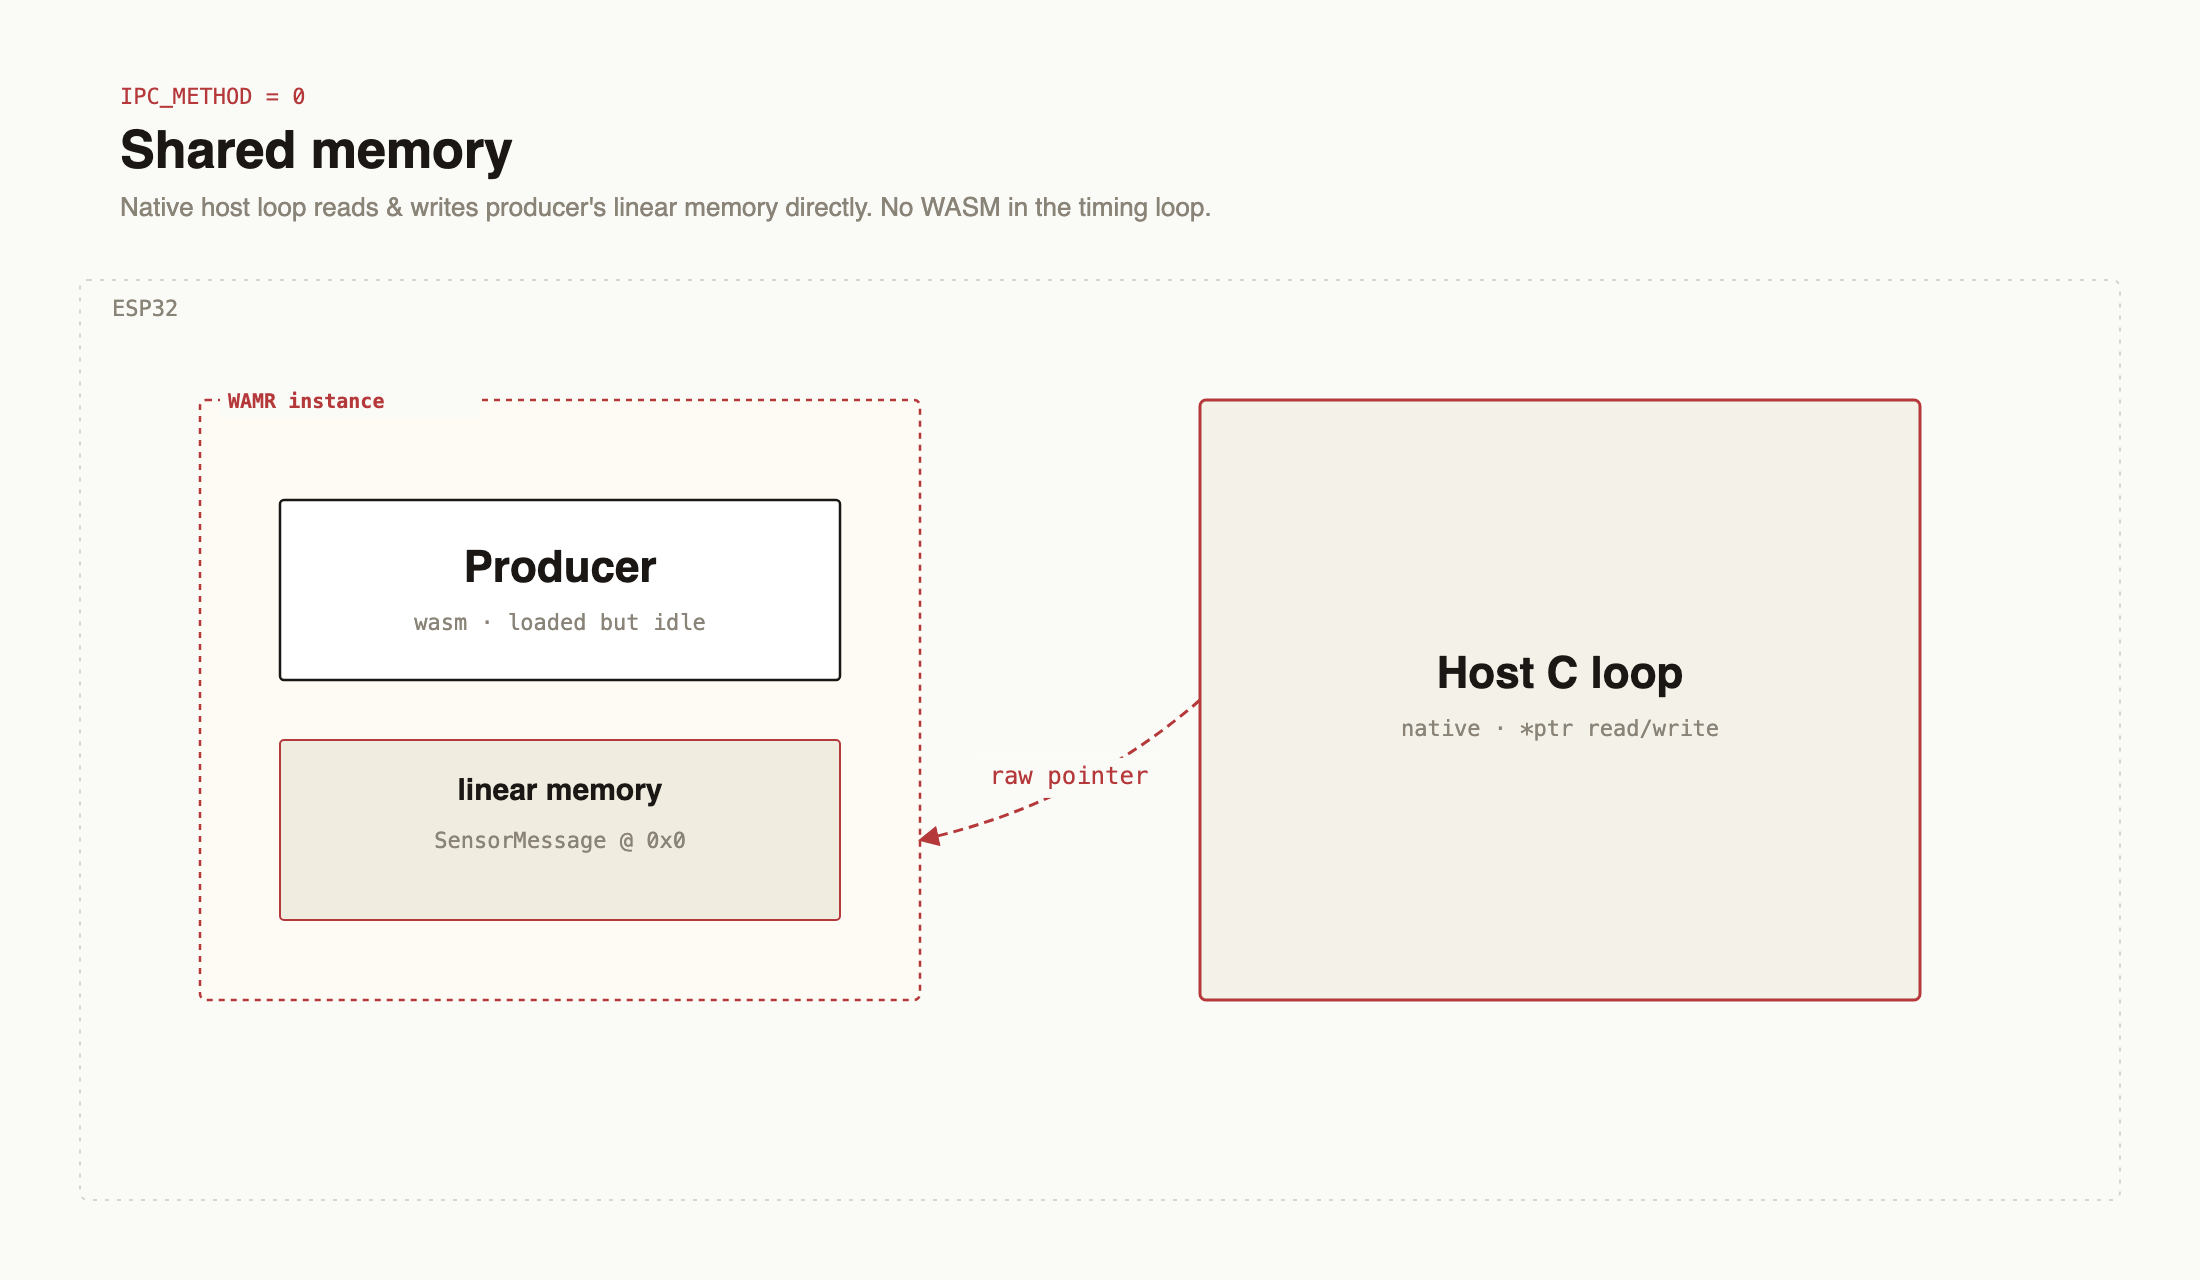
\includegraphics[width=\textwidth]{images/m0.png}
    \caption{Shared memory}
    \label{fig:ipc-m0}
  \end{subfigure}
  \hfill
  \begin{subfigure}[t]{0.32\textwidth}
    \centering
    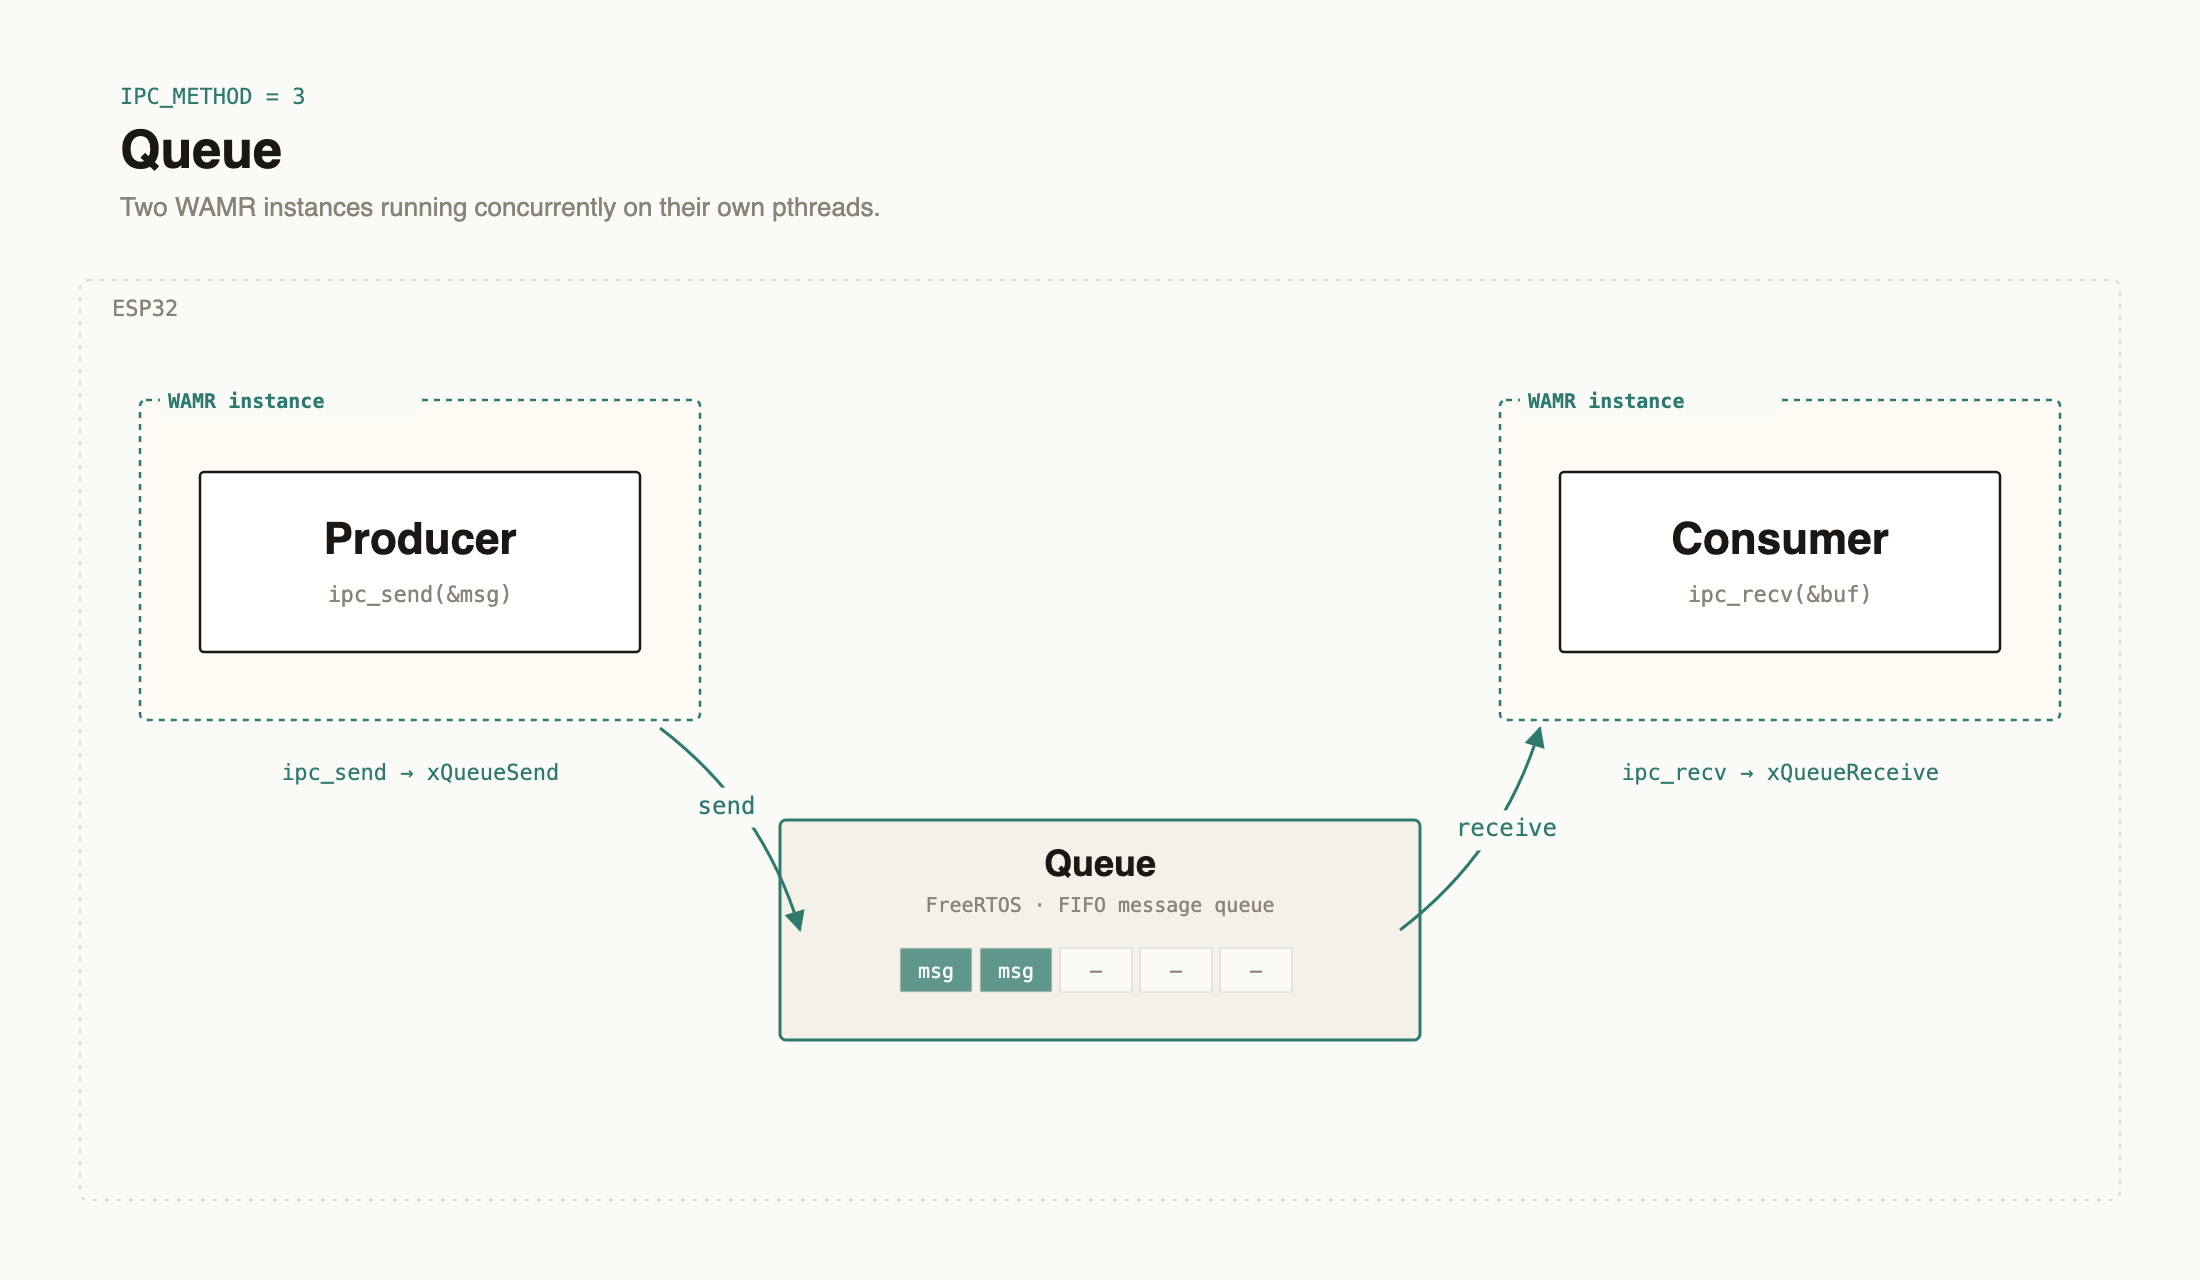
\includegraphics[width=\textwidth]{images/m3.png}
    \caption{Queue}
    \label{fig:ipc-m3}
  \end{subfigure}
  \hfill
  \begin{subfigure}[t]{0.32\textwidth}
    \centering
    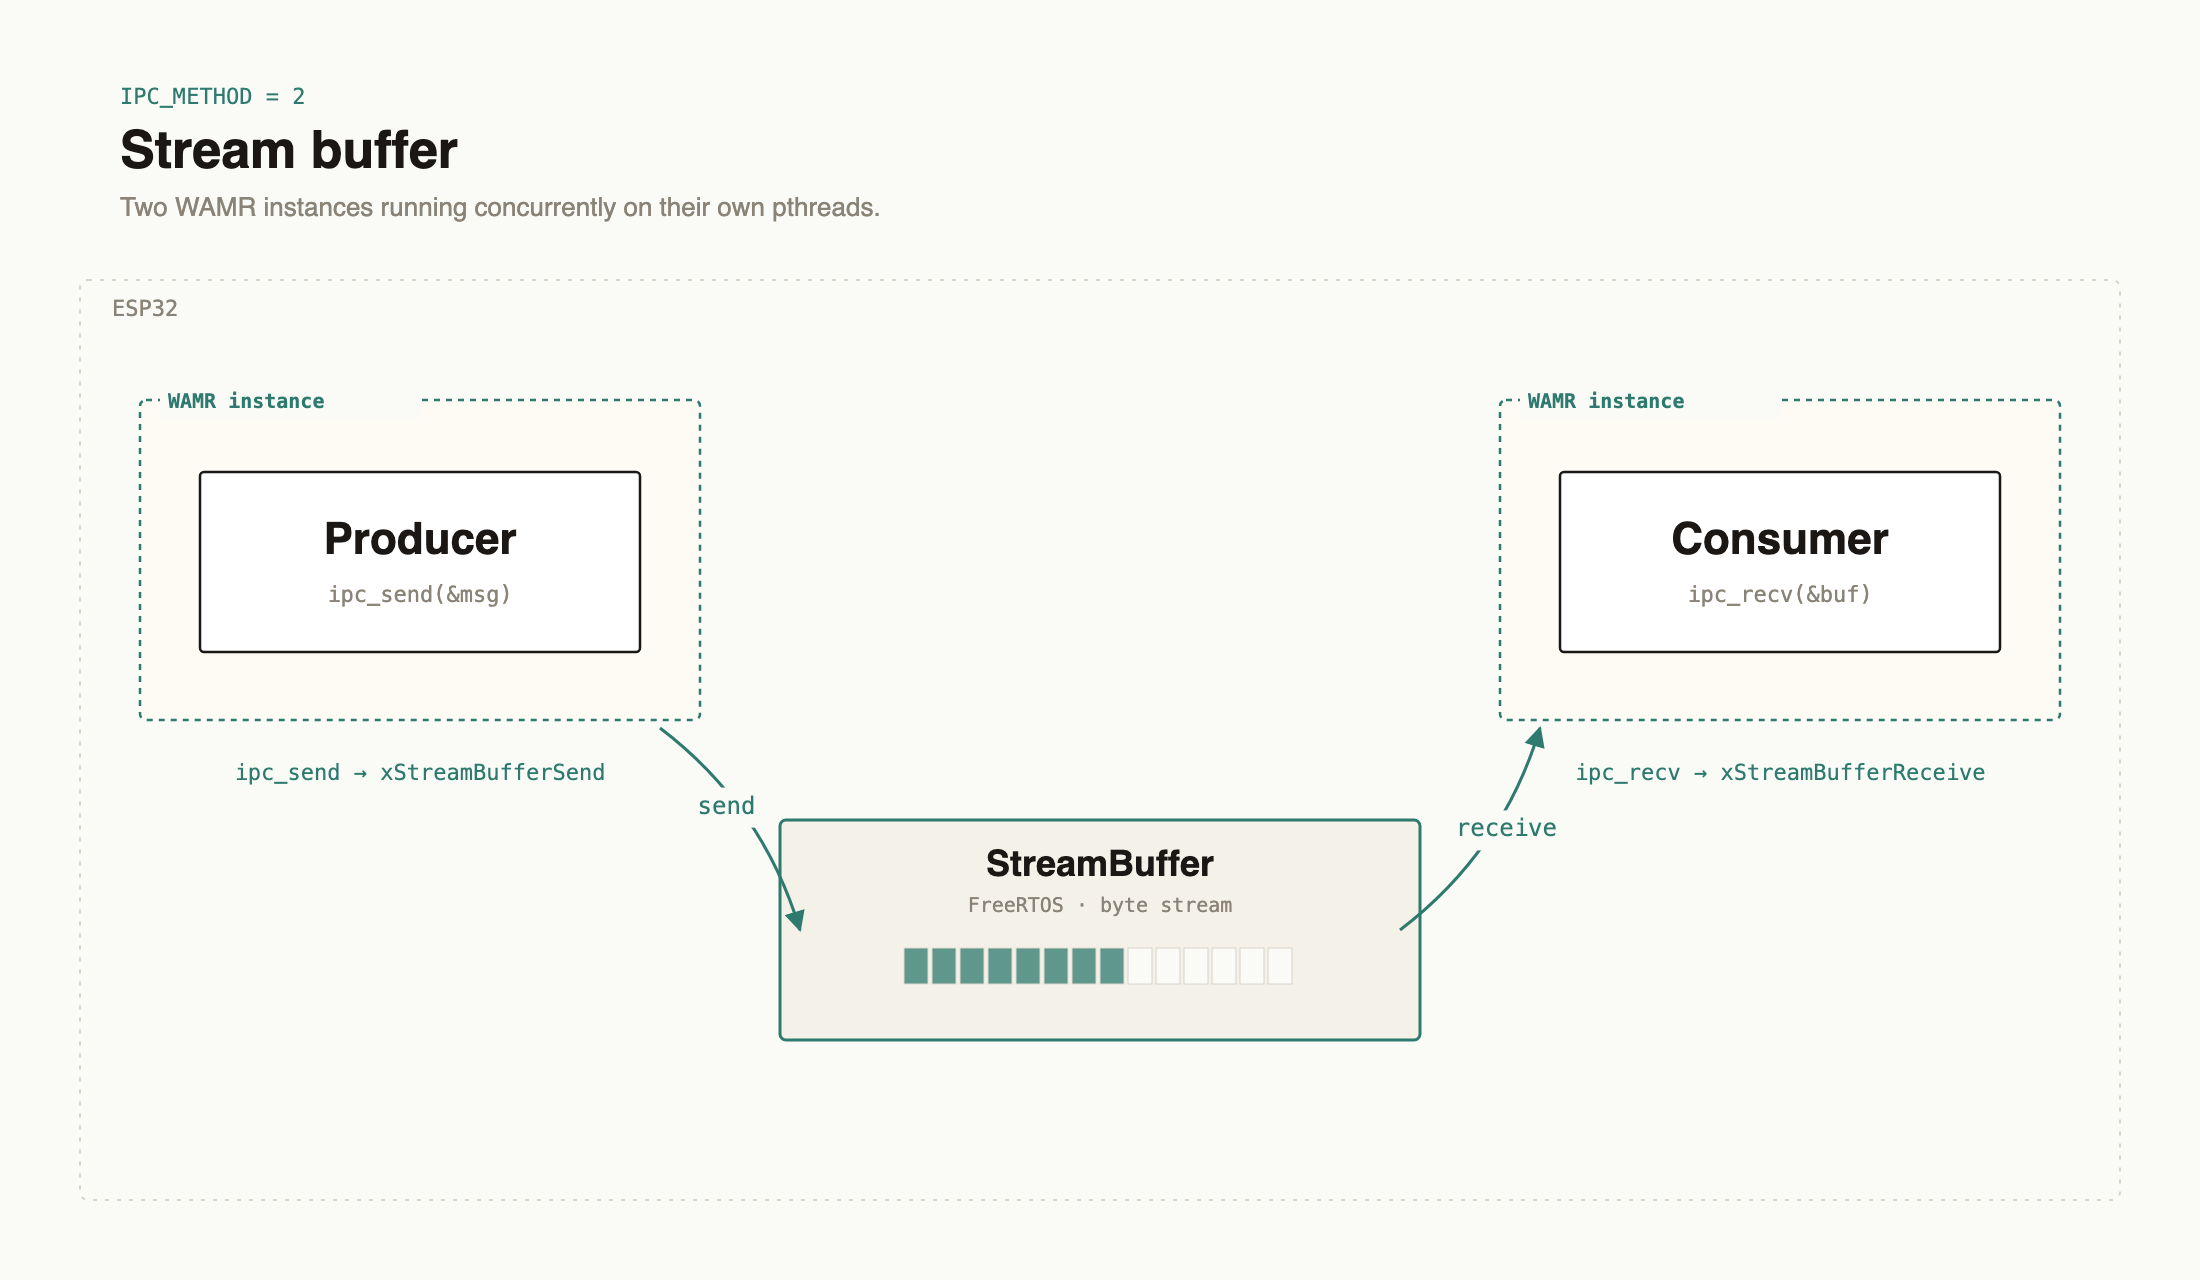
\includegraphics[width=\textwidth]{images/m2.png}
    \caption{Stream buffer}
    \label{fig:ipc-m2}
  \end{subfigure}

  \vspace{0.6em}

  \begin{subfigure}[t]{0.40\textwidth}
    \centering
    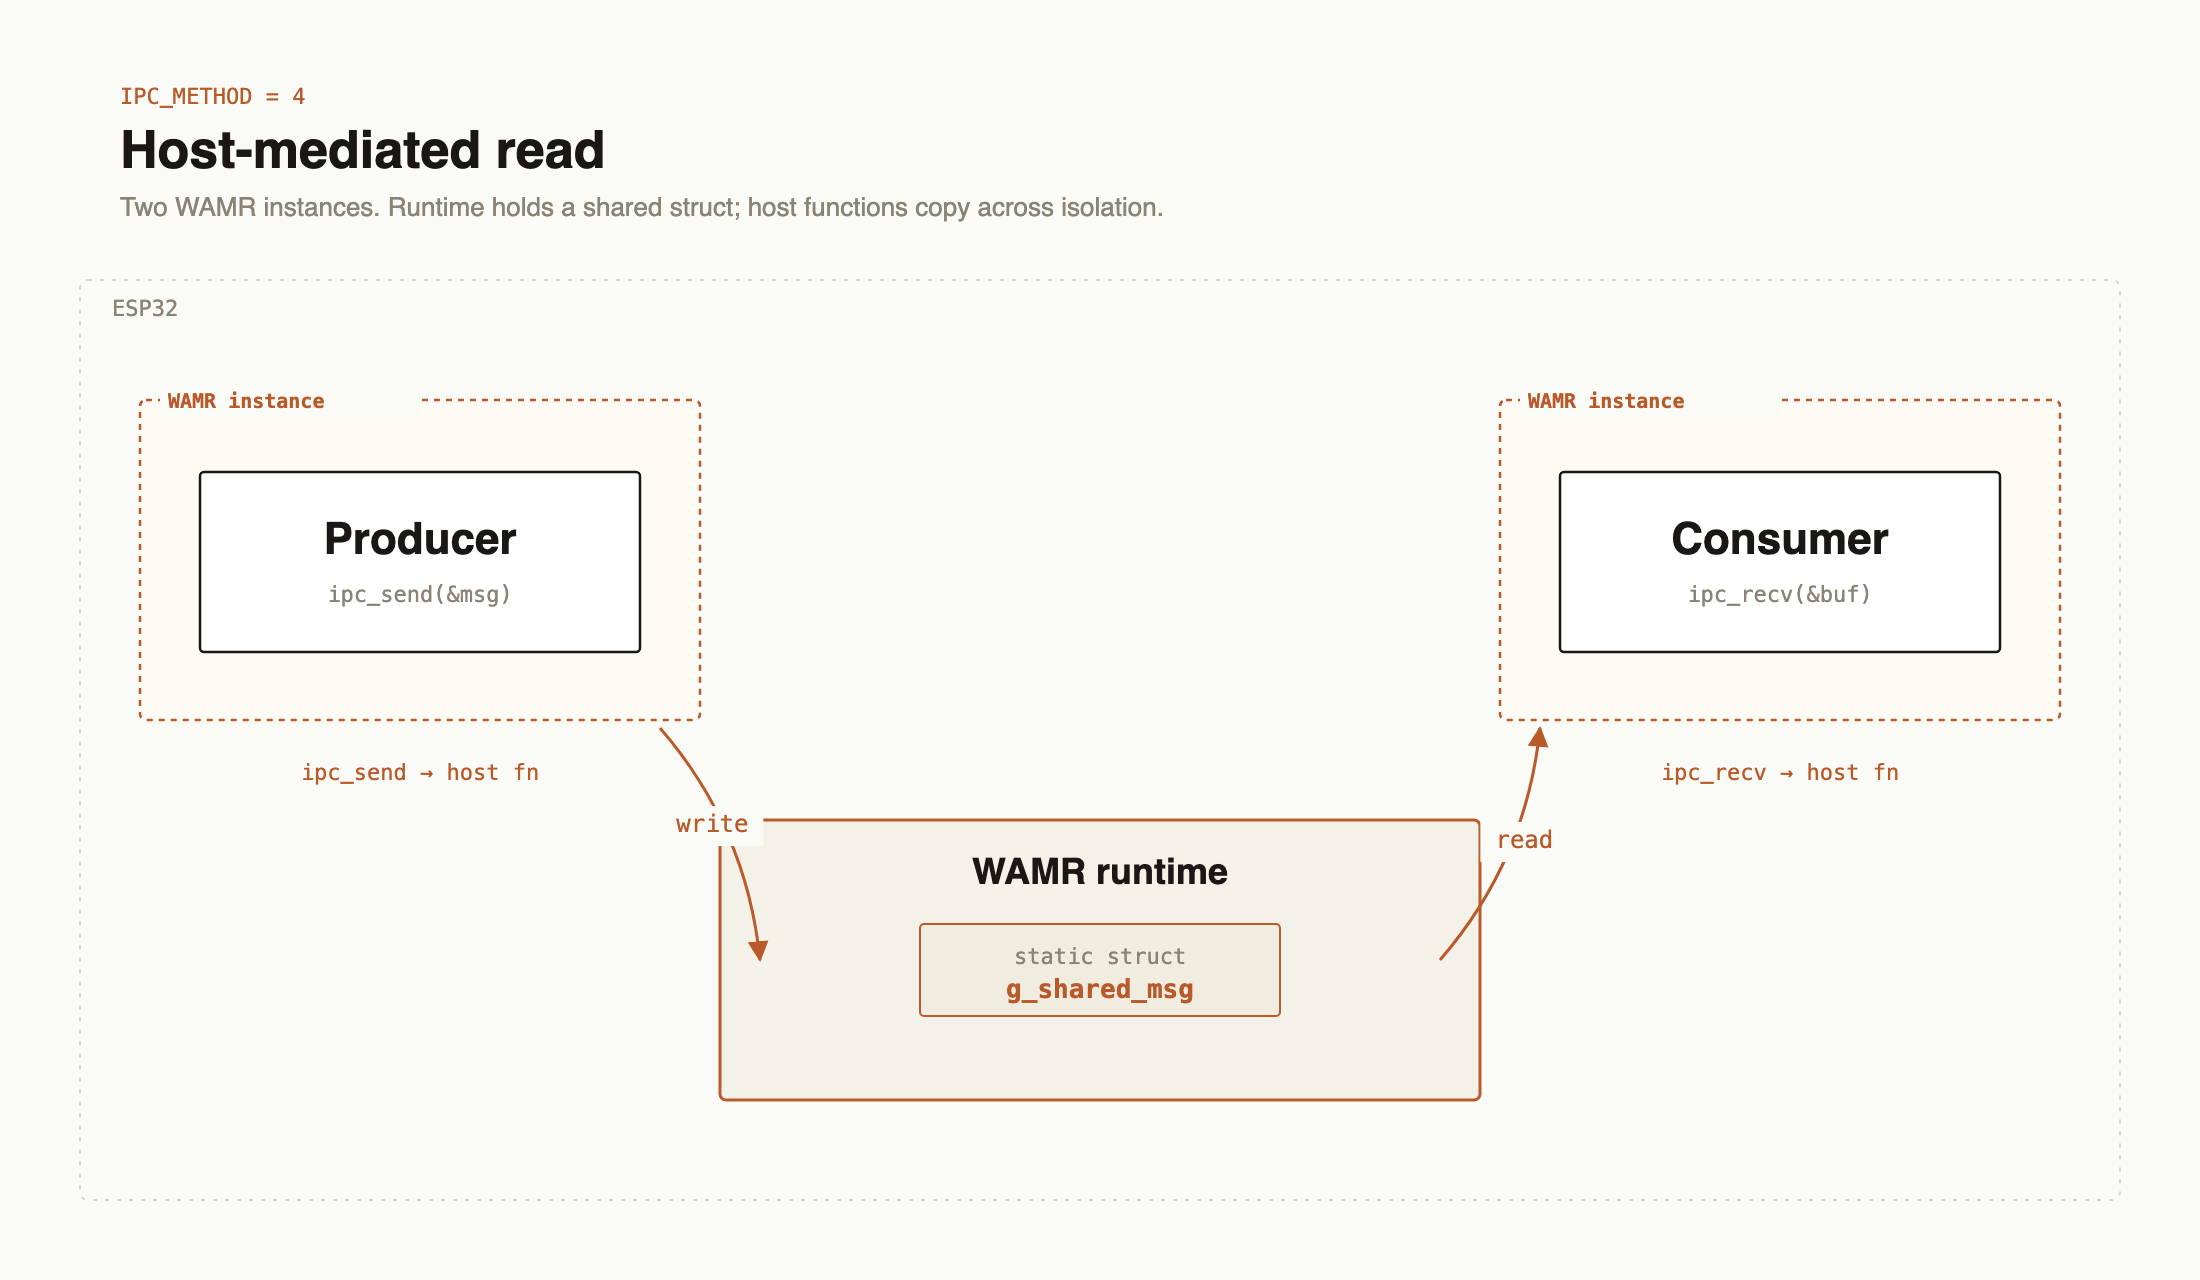
\includegraphics[width=\textwidth]{images/m4.png}
    \caption{Host-mediated read}
    \label{fig:ipc-m4}
  \end{subfigure}
  \hfill
  \begin{subfigure}[t]{0.40\textwidth}
    \centering
    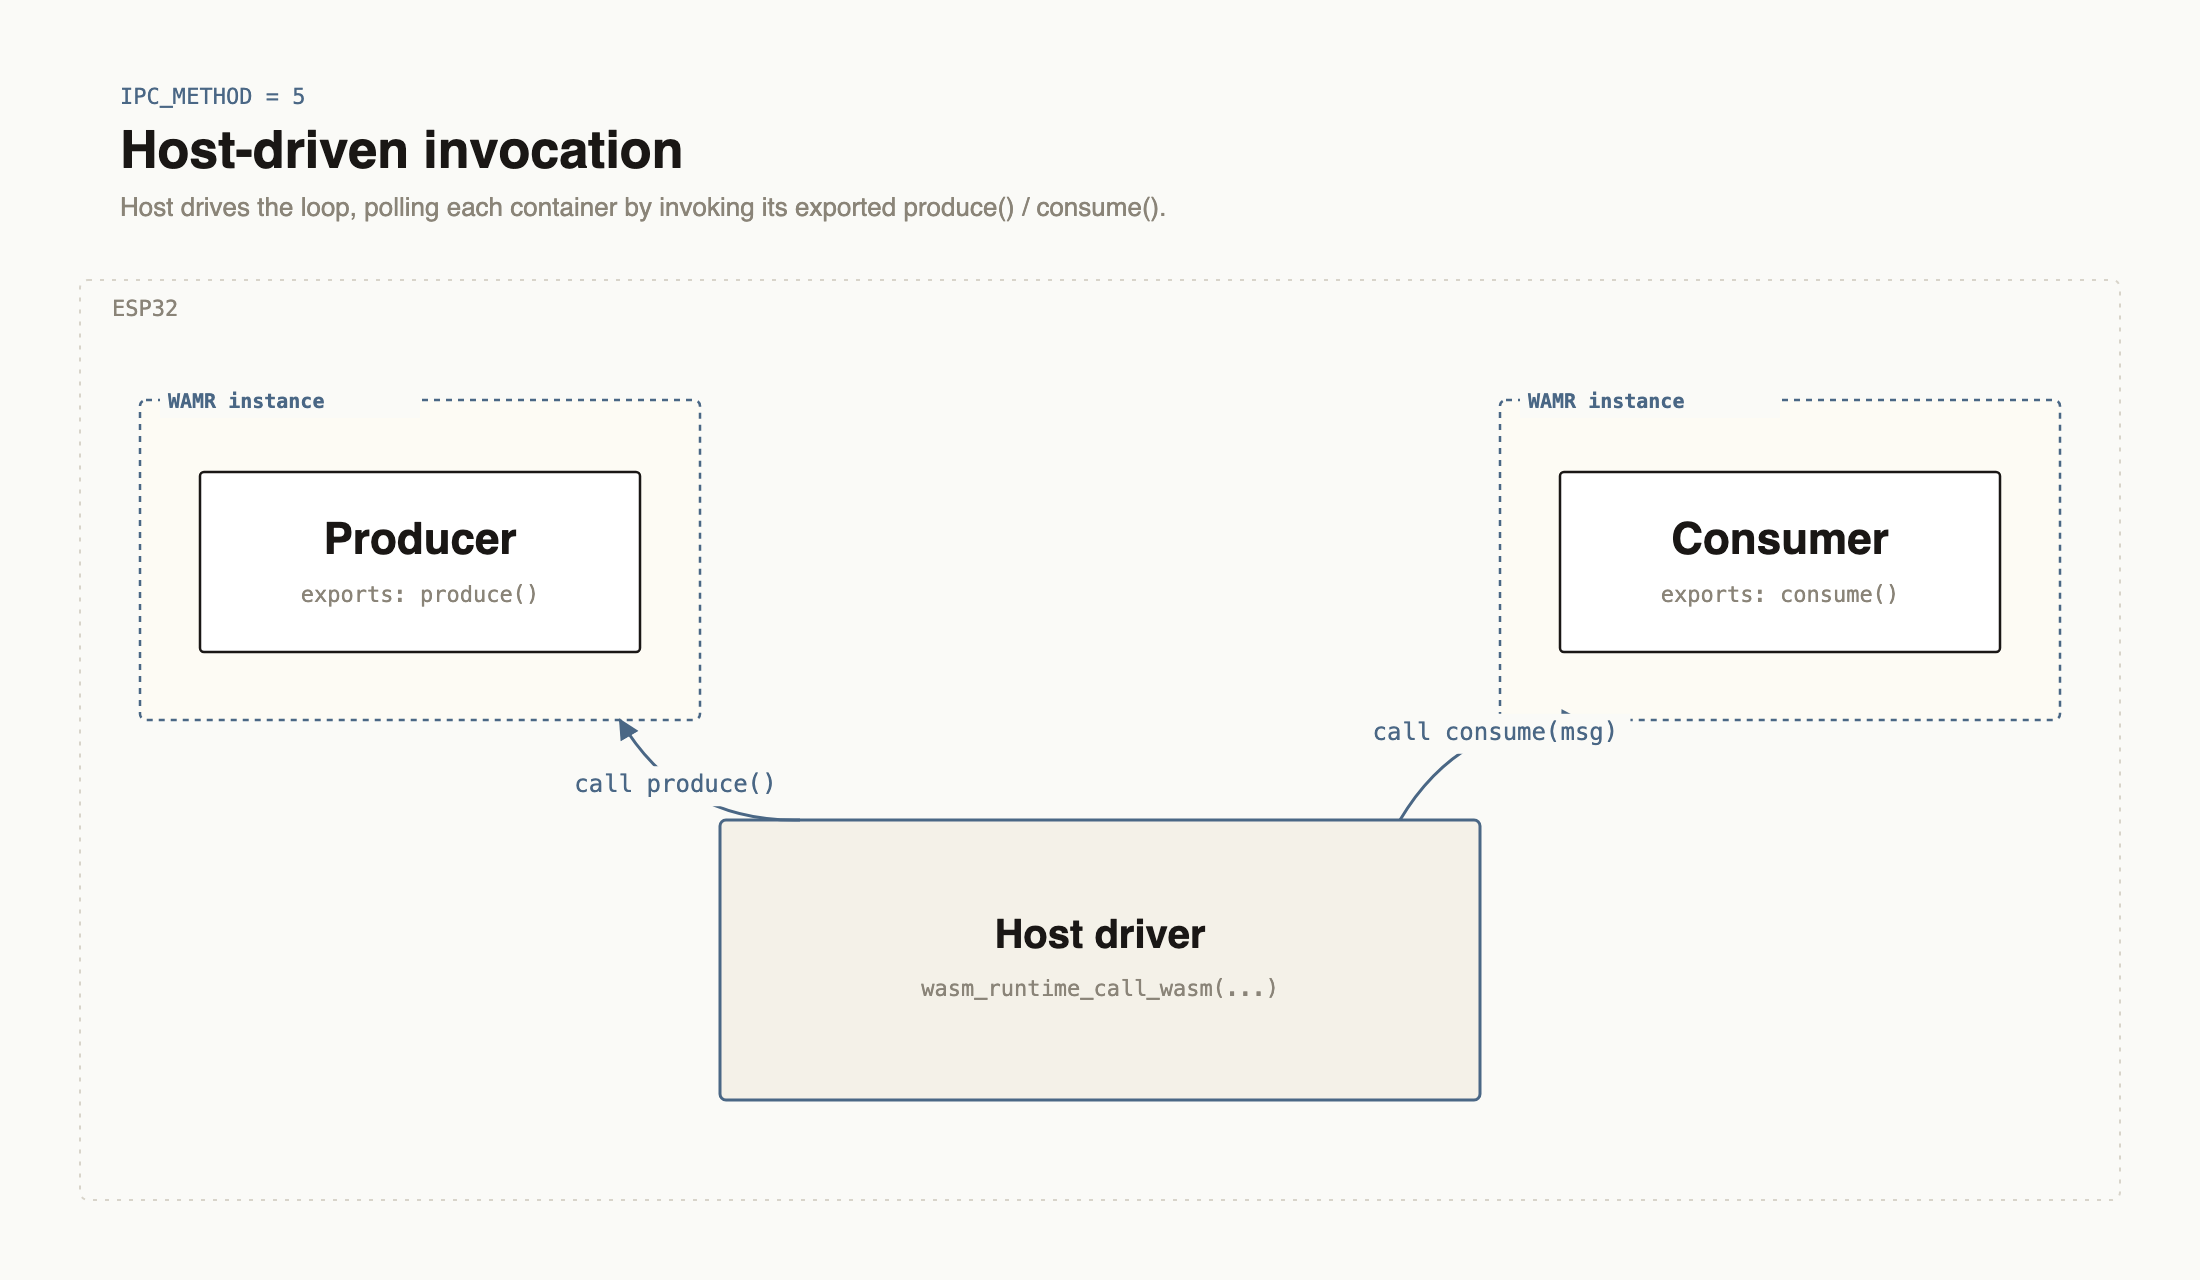
\includegraphics[width=\textwidth]{images/m5.png}
    \caption{Host-driven invocation}
    \label{fig:ipc-m5}
  \end{subfigure}
  \caption{IPC architectures evaluated in the containerisation benchmark.}
  \label{fig:ipc-architectures}
\end{figure}

\subsection{Metrics}
\label{subsec:containerization-ipc-metrics}

Per-iteration cost is measured using the Xtensa CPU's CCOUNT register, a free-running 32-bit counter that increments once per CPU clock tick and is readable through the single-instruction \texttt{rsr.ccount} macro. Reading CCOUNT immediately before and after each operation gives cycle-exact timing with a resolution of 4.17\,ns at 240\,MHz, tight enough to distinguish a bare pointer dereference from a WAMR-mediated read without the measurement itself dominating the quantity being measured. Each run captures the following.

\begin{itemize}
  \item \textbf{Per-iteration cycles:} Each iteration records three numbers. \texttt{write\_cycles} is the CCOUNT delta around the producer-side operation, whether that is a raw store, \texttt{xQueueSend}, \texttt{xStreamBufferSend}, or the host-function write. \texttt{read\_cycles} is the matching delta around the consumer-side operation. \texttt{round\_trip\_cycles} is their sum, and that is the figure the results table reports, since the end-to-end cost per message is what constrains how the IPC fits into a loop. 10{,}000 iterations are recorded per architecture, and the summary CSVs contain the min, max, mean, p50, p95, and p99 of that distribution. The tail statistics matter more than the mean for control-loop scheduling, because the worst case determines the jitter floor.
  \item \textbf{Free heap:} Free heap reading at the start and end of each run, sampled through \texttt{esp\_get\_free\_heap\_size()}. The delta across the run reveals whether the architecture leaks memory; the absolute level indicates the RAM cost of the isolation mechanism itself.
  \item \textbf{Core affinity:} Whether the producer and consumer were pinned to the same core or to separate cores, controlled through \texttt{xTaskCreatePinnedToCore}. All figures below use the same-core configuration; cross-core runs were collected but do not change the ordering of the methods.
\end{itemize}

\subsection{Result}
\label{subsec:containerization-ipc-results}

Table~\ref{tab:ipc-methods-p52} shows the per-iteration cost of each IPC architecture at a 52-byte payload. The mean column is the cycle count averaged across 10{,}000 iterations, converted to microseconds at 240\,MHz, and the ratio column expresses the gap to the shared-memory baseline.

\begin{table}[htbp]
\centering
\small
\begin{tabular}{@{}lrrrrrr@{}}
\toprule
\textbf{Method} & \textbf{Mean} & \textbf{Mean} & \textbf{p50} & \textbf{p95} & \textbf{p99} & \textbf{Ratio} \\
 & \textbf{(cycles)} & \textbf{(\textmu{}s)} & \textbf{(cycles)} & \textbf{(cycles)} & \textbf{(cycles)} & \textbf{vs shm} \\
\midrule
Shared memory   & 25.2       & 0.11   & 25      & 25      & 25      & 1$\times$ \\
Host-mediated read     & 16{,}974.8 & 70.7   & 16{,}717 & 17{,}951 & 18{,}645 & 673$\times$ \\
Queue                  & 49{,}241.1 & 205.2  & 19{,}433 & 288{,}318 & 428{,}928 & 1{,}954$\times$ \\
Stream buffer          & 59{,}612.1 & 248.4  & 20{,}846 & 345{,}699 & 416{,}795 & 2{,}366$\times$ \\
Host-driven invocation & 419{,}763.4 & 1{,}749.0 & 419{,}778 & 420{,}839 & 421{,}026 & 16{,}657$\times$ \\
\bottomrule
\end{tabular}
\caption{Per-iteration cost of each IPC architecture at a 52-byte payload, same-core, 10{,}000 iterations. Ratios are computed against the shared-memory mean.}
\label{tab:ipc-methods-p52}
\end{table}

\paragraph{Shared memory:} At around 25 cycles per iteration, the measurement is the cost of a native store followed by a native load issued by the host through a pointer into a single container's linear memory. No WASM executes in the timing loop and no module boundary is crossed. The p50, p95, and p99 are identical, so the access path has no observable jitter. This is a reference point for what raw memory access costs on the platform, not a realistic multi-container architecture.

\paragraph{Host-mediated read:} The host-mediated read costs around 70\,\textmu{}s per message, roughly 673$\times$ the shared-memory baseline. Its tail behaviour is tightly controlled: p99 sits within 12\% of the p50. Each exchange is two host-function calls and two memory copies through \texttt{wasm\_runtime\_addr\_app\_to\_native} --- the producer into the host-owned buffer, the consumer out of it --- all of which run deterministically without involving the scheduler. For control-loop periods in the tens to hundreds of milliseconds this is comfortably within budget.

\paragraph{Queue and stream buffer:} The two RTOS-mediated methods share a structural signature: their medians, around 19--21\,k cycles, are close to the host-mediated read, but their p95 and p99 values jump to 270--460\,k cycles. The mean is three times the median in each case, which is the clearest possible sign that the distribution is dominated by rare but expensive scheduler interactions. Each message involves a context switch between the producer and consumer tasks, and the scheduler's latency is sensitive to whatever else is running. A 400\,k-cycle worst-case event is roughly 1.7\,ms of blocked time on CPU0 --- a substantial fraction of a 10\,ms control period.

\paragraph{Host-driven invocation:} The host-driven invocation path costs around 420\,k cycles (1.75\,ms) per message and is the highest-overhead architecture tested. The cost is the full host$\to$guest call path: argument marshalling, stack-frame setup, and a WASM function dispatch per message. It is also the most consistent of the mediated methods: p99 is within 0.3\% of the mean, because no scheduler is involved. The mechanism honours the sandbox boundary on every exchange, and the cost reflects exactly that.

\paragraph{Memory footprint:} Free-heap readings separate the architectures into three tiers. Shared memory runs with 104\,kB free because only one container is instantiated; the host reads and writes directly into that container's linear memory through a native pointer, and no second module or exec\_env is allocated. The other methods each instantiate two containers and thus have 63\,kB of free heap, which is the cost of reserving a second linear-memory region and its module instance.

\subsection{Payload sensitivity}
\label{subsec:containerization-payload}

Table~\ref{tab:ipc-payload} shows the mean cycle count as the payload grows from 0 to 244 bytes. For every method the payload effect is smaller than the run-to-run variation in the mean.

\begin{table}[htbp]
\centering
\small
\begin{tabular}{@{}lrrr@{}}
\toprule
\textbf{Method} & \textbf{0\,B} & \textbf{52\,B} & \textbf{244\,B} \\
\midrule
Shared memory   & 25.2       & 25.2       & 25.3 \\
Host-mediated read     & 17{,}047.4 & 16{,}974.8 & 17{,}013.1 \\
Queue                  & 49{,}580.4 & 49{,}241.1 & 43{,}512.1 \\
Stream buffer          & 58{,}487.4 & 59{,}612.1 & 60{,}094.1 \\
Host-driven invocation & 419{,}763.3 & 419{,}763.4 & 419{,}171.1 \\
\bottomrule
\end{tabular}
\caption{Mean cycles per iteration as a function of payload size. }      
\label{tab:ipc-payload}
\end{table}

The implication is that the overhead measured here is almost entirely agnostic of the size of the message while runtime mediation, scheduler interaction, and choice of IPC are visible in the measured results.

\section{Container-count scaling}
\label{sec:containerization-scaling}

The IPC benchmark shows what each message costs once a workload is split across containers. A different question is how many containers can stay active at once before the ESP32 out of memory or scheduler headroom. To answer that, a separate scaling benchmark was added to the same host project and run in both interpreter and AOT modes.

\subsection{Methodology}
\label{subsec:containerization-scaling-method}

The benchmark loads the same worker module from SPIFFS $N$ times, instantiates $N$ separate WAMR module instances, creates one \textbf{exec\_env} and one host \textbf{pthread} per instance, and releases all workers together through a start barrier. 

Each container runs the same deterministic integer-only kernel. In the final version used here, the worker performs 120 outer iterations; each iteration executes 2{,}048 inner arithmetic rounds, yields cooperatively to the host every 512 rounds, and then calls a 15~ms host delay. The checksum reported at the end of the run is fixed, so completion is only accepted if every container reaches the expected final state.

\begin{algorithm}[htbp]
  \caption{CPU-bound worker kernel used by each container}
  \label{alg:container-worker-kernel}
  \begin{algorithmic}[1]
  \Procedure{WorkerContainer}{$container\_id, iterations, inner\_work$}
      \State $checksum \gets container\_id$
      \For{$i \gets 0$ to $iterations - 1$}
          \State $x \gets i + container\_id$
          \For{$j \gets 0$ to $inner\_work - 1$}
              \State $x \gets x \times 1664525 + 1013904223$
              \State $x \gets x \oplus (x \gg 16)$
              \State $x \gets x + j$
          \EndFor
          \State $checksum \gets checksum \oplus x$
          \If{$i \bmod sample\_interval = 0$}
              \State \Call{ReportProgress}{$container\_id, i, checksum$}
          \EndIf
      \EndFor
      \State \Return $checksum$
  \EndProcedure
  \end{algorithmic}
\end{algorithm}

For each container count, the benchmark tracks free heap at five points: before WAMR initialisation, after initialisation, after loading the $N$ modules, after instantiating them, and at the lowest point reached during steady-state execution. It also records the total startup time for the full container set and samples mean CPU utilisation from FreeRTOS runtime statistics while the workers are active. The sweep increments $N$ until a run fails or becomes unstable. A run is treated as unstable if any worker fails to finish within the 15~s timeout, or if the task watchdog fires because the worker tasks starve the idle task.

\subsection{Results}
\label{subsec:containerization-scaling-results}

The interpreter remained stable up to six concurrent containers and failed at seven with a timeout. AOT remained stable up to eleven containers and failed at twelve when the host could no longer create another pthread. The full per-container measurements are provided in Appendix~\ref{app:scaling-tables}.

\begin{figure}[htbp]
  \centering
  \begin{subfigure}[t]{0.49\textwidth}
      \centering
      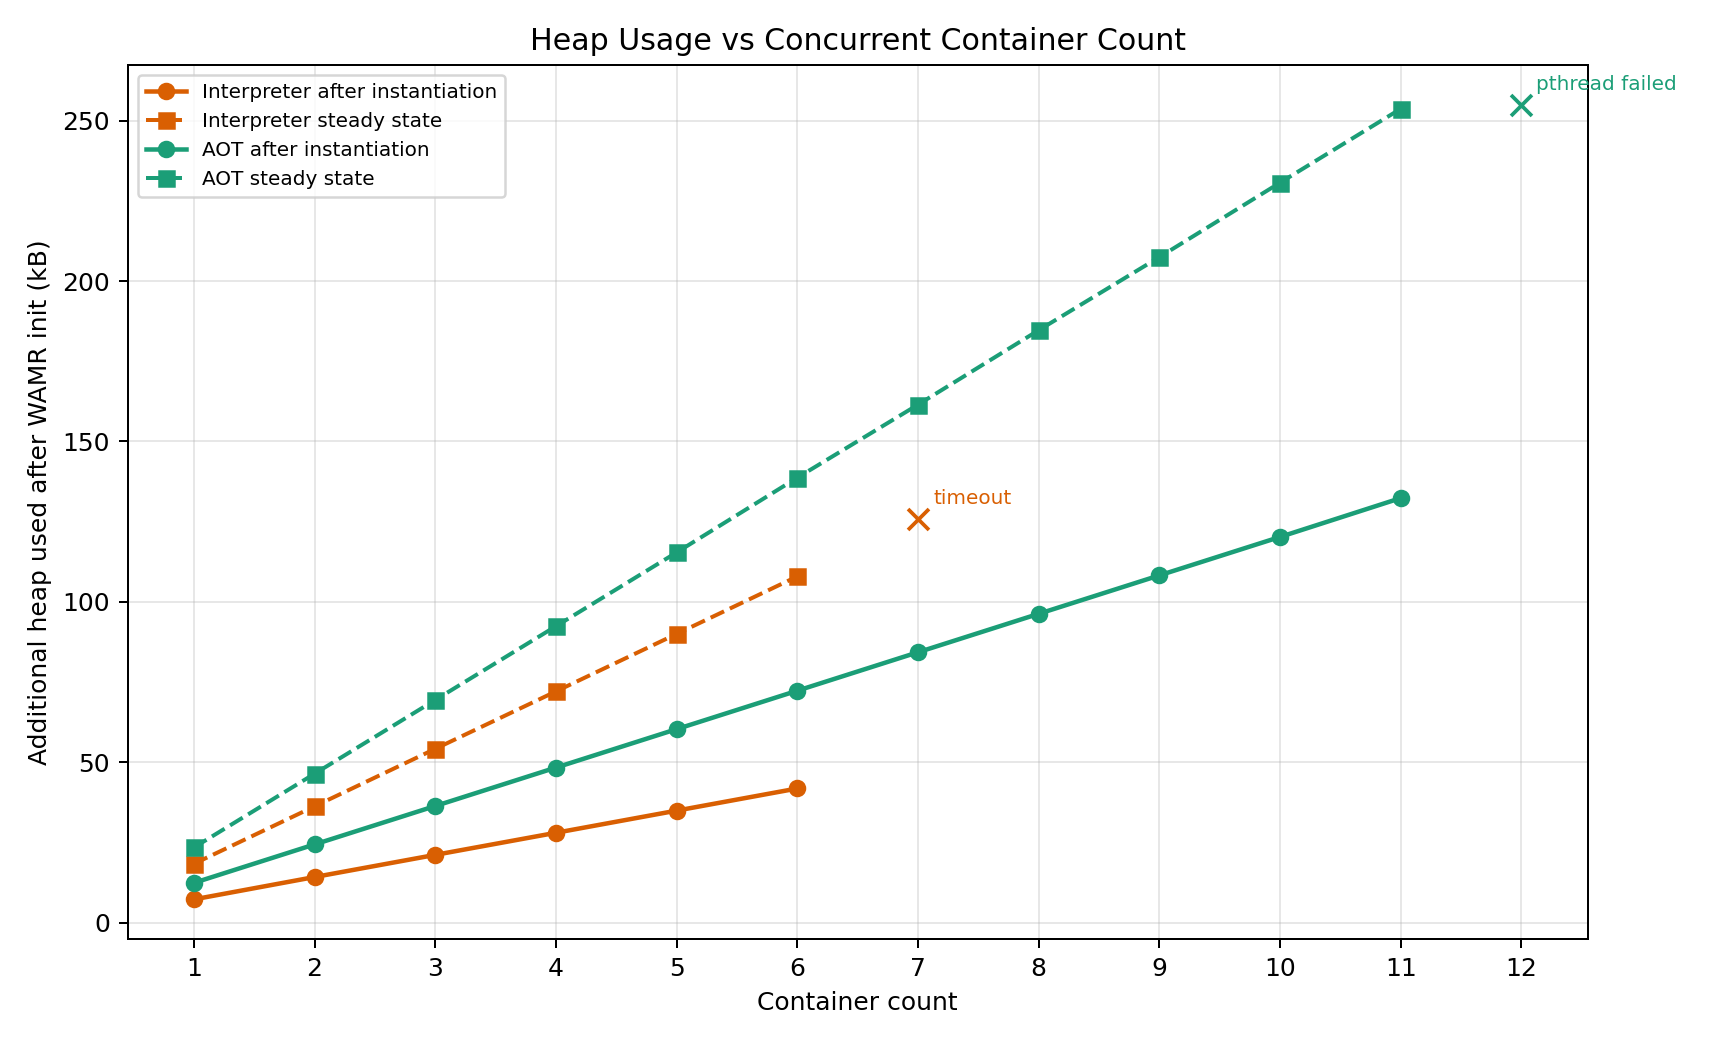
\includegraphics[width=\textwidth]{images/container_scaling_heap.png}
      \caption{Heap usage}
      \label{fig:container-scaling-heap}
  \end{subfigure}
  \hfill
  \begin{subfigure}[t]{0.49\textwidth}
      \centering
      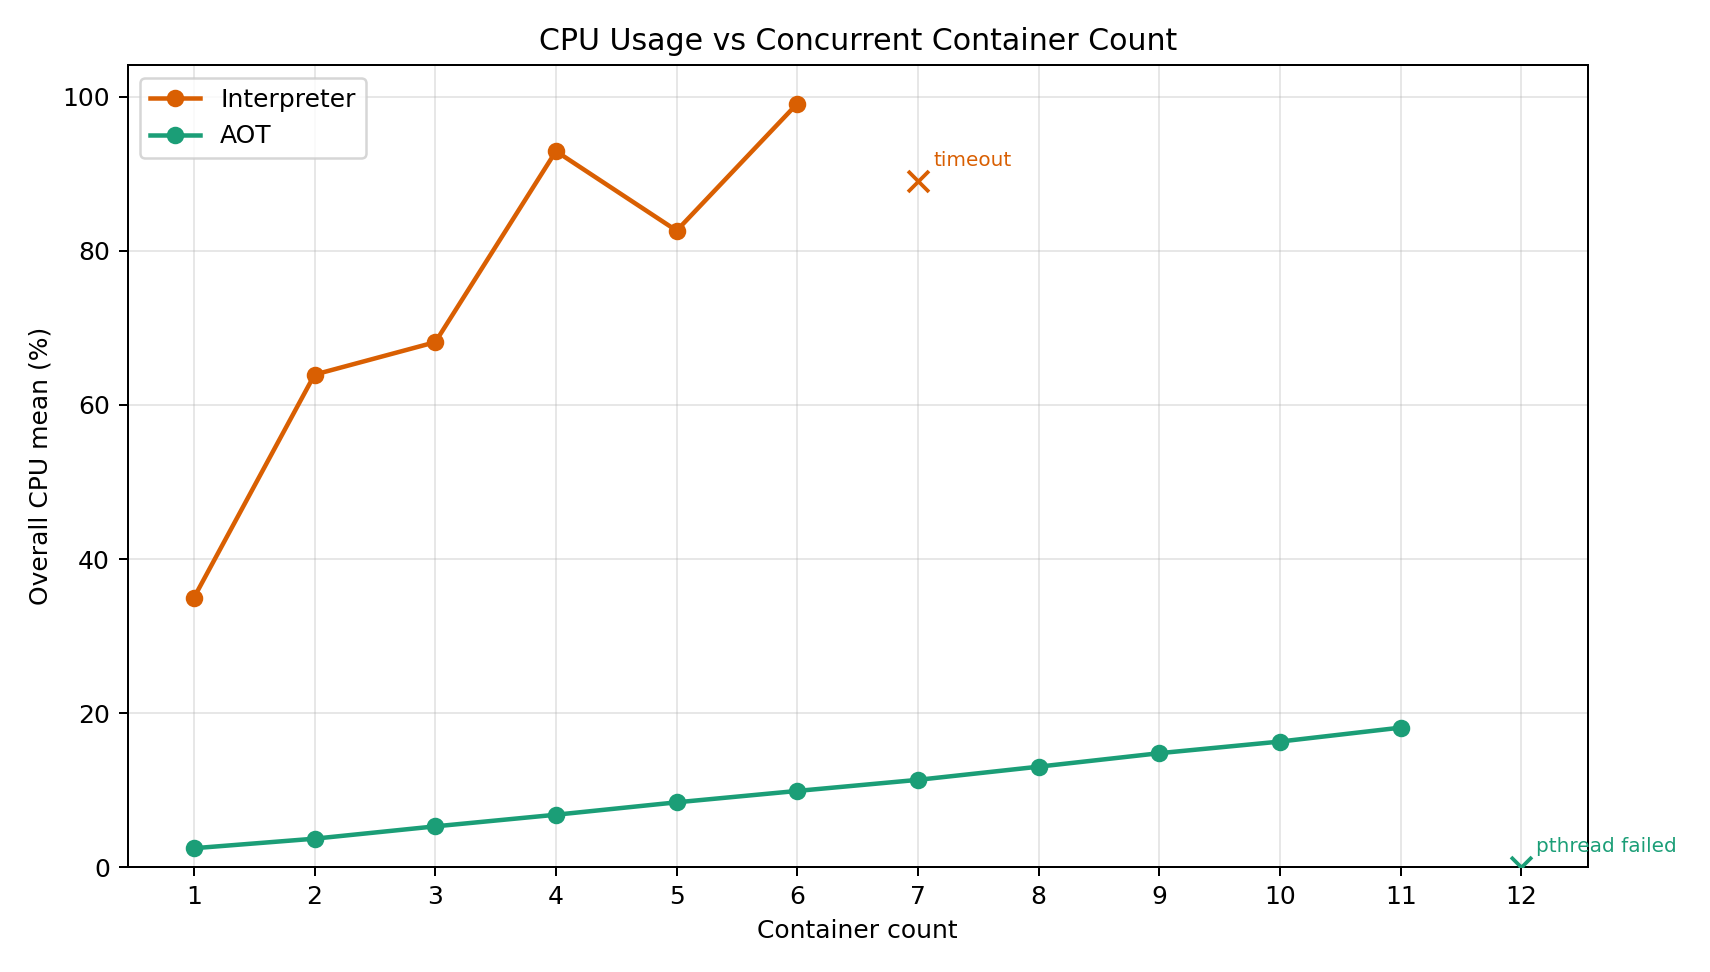
\includegraphics[width=\textwidth]{images/container_scaling_cpu.png}
      \caption{CPU utilisation}
      \label{fig:container-scaling-cpu}
  \end{subfigure}
  \caption{CPU & heap usage against container count for WAMR on the ESP32.}
  \label{fig:container-scaling}
\end{figure}

Figure~\ref{fig:container-scaling} shows the corresponding memory and CPU trends. The memory trend is close to linear in both modes over the successful part of the sweep, but the slopes are different. Using a straight-line fit over the successful runs, free heap after instantiation drops by about 6.9\,kB per added interpreter container and about 12.0\,kB per added AOT container. The steady-state slope is steeper because the exec\_env objects and pthread stacks are live while the workers are running: about 17.9\,kB per active interpreter container and 23.0\,kB per active AOT container. 

CPU behaviour is what separates the two modes in practice. Interpreter mode rises from 35.0\% overall CPU utilisation at $N=1$ to 99.1\% at $N=6$, and the first unstable run appears at $N=7$. That failure did not happen because memory was exhausted as 131.9\,kB of free heap was still visible at the lowest point of the run. The limiting factor was scheduler starvation. The task watchdog fired while a benchmark pthread was running on each core inside WAMR's bytecode interpreter, and the run eventually hit the benchmark timeout. AOT shows the opposite pattern. Its CPU load remains low across the whole successful range, rising from 2.4\% at $N=1$ to 18.1\% at $N=11$, and the failure boundary is pushed out to $N=12$, where pthread creation fails with only 2.9\,kB of free heap remaining. For AOT, the practical limit is memory rather than CPU.

Startup time also scales roughly linearly with the number of containers. The fitted slope is about 3.3~ms per added container in interpreter mode and 5.2~ms per added container in AOT mode. The AOT startup slope is steeper because the module image is larger (15kB compared with 490B) and its instantiation work costs more, but that extra startup cost is small compared with the difference in execution overhead once the workers are running.


\section{Discussion}
\label{sec:containerization-discussion}

Three things follow from these results. One is how firmware is updated, one about how containers communicate with each other, and one about how far a modular design can be pushed on this class of microcontroller.

If the platform code remains stable between releases and only the control logic changes, placing the algorithm in a Wasm container turns a field update into a 7.6\,s SPIFFS write rather than a 20\,s full flash. It also reduces the 59\,s build-plus-flash developer cycle to a container reload on the host. The update payload falls from 1.02\,MB to 512\,kB, which matters on low-bandwidth links such as LoRaWAN and can reduce aggregate bandwidth consumption across a fleet. The safety boundary also improves. A SPIFFS-only update does not touch the bootloader or application partition, so a bad container can fail to load while the host keeps running the previous version. On the other hand, as demonstrated in Chapter \ref{ch:fault_tolerance} a bad firmware image can crash the whole ESP32 device.

The IPC results show that the communication method matters more than the message size for the payloads tested. Taking shared memory as the baseline, the four IPC designs differ by an order of magnitude in cost, mainly because they impose different amounts of isolation and scheduler involvement per message. Host-mediated read is the cheapest stable option because each exchange is handled as a deterministic copy through a host-owned buffer, without waking another task. Queues and stream buffers allow producer and consumer containers to run concurrently, but this concurrency comes with occasional long delays when context switches occur. Host-driven invocation has the highest average cost because the host crosses into and out of the Wasm sandbox for every message, but its timing is more consistent because the scheduler is not on the critical path. These results do not exhaust the possible IPC designs, but they show that, for modular Wasm workloads on the ESP32, the communication architecture is a major performance consideration.

The scaling benchmark adds a second architectural constraint. In interpreter mode, the first hard limit is CPU time rather than available memory. The ESP32 still had well over 100\,kB of free heap when the seven-container run became unstable, since the workers spent too much time inside the bytecode interpreter and starved the idle task, causing the task watchdog to fire. With AOT, the bottleneck changes. CPU headroom remains comfortable, but each additional container consumes enough resident memory that the twelfth worker fails during pthread creation. Therefore, for workloads that require several concurrently active containers on the ESP32, AOT is the practical mode. Interpreter mode is better suited to smaller container counts or less aggressive concurrent workloads.

% ============================================================


% ============================================================
\chapter{Conclusions}
\label{ch:conclusion}

\section{Summary of findings}

This project evaluated whether WebAssembly can provide a practical modular execution layer for embedded control workloads on an ESP32. The answer is conditional. For the thermal-control workloads studied here, WebAssembly preserved the required control behaviour at the tested timing budget and provided useful system-level benefits. The cost was mainly memory, with smaller but measurable overheads in host calls, execution time, CPU activity, and end-to-end latency.

The performance results show that WebAssembly was feasible for the tested closed-loop workload. At a 100 ms control period, both WAMR interpreter and WAMR ahead-of-time (AOT) execution produced the same control behaviour as the native C baseline. The runtime overhead was visible in fine-grained measurements rather than in the thermal response itself. Interpreter mode added about 59~\textmu{}s to a temperature read and 113~\textmu{}s to a heater write over native execution, while AOT reduced those penalties to about 23--25~\textmu{}s. The total wall-clock overhead stayed below 0.2\%, largely because the workloads were dominated by deliberate timing delays rather than computation. The more significant cost was SRAM: WAMR consumed about 76--86~KB of additional memory compared with native execution.

These findings are consistent with prior embedded-Wasm work, but move the discussion beyond whether Wasm can execute on a microcontroller. The contribution of this project is that it quantifies the cost of WebAssembly at both granular and system levels on a ESP32 within the context of a simulated workload. The evaluation separates host-function overhead, loop timing, end-to-end signal latency, memory footprint, CPU activity, fault recovery, update cost, IPC behaviour, and multi-container scaling. This makes the result more useful than a single native-versus-Wasm slowdown figure as it identifies where overhead enters the system, which costs matter for control behaviour, and which resources become limiting as the system architecture becomes more modular.

The fault-injection results show the clearest system-level benefit of the runtime. In the native firmware, representative faults such as null-pointer access, stack overflow, and infinite loop conditions caused system-level failure and reset. Under WAMR, the same classes of fault were contained at the container boundary and recovered without rebooting the device. The important difference is therefore not only that the fault was detected, but that recovery happened at the container level while the host firmware and long-lived system tasks remained alive.

The deployment experiments also support the modular-firmware argument. Updating only the container partition was substantially cheaper than reflashing the whole firmware image: the SPIFFS-only update path took about 7.60~s, compared with 20.15~s for a full flash and 59.04~s for build plus flash. This matters when the changed component is application logic rather than device support code. In that case, a Wasm-based design allows the control algorithm to be replaced without rebuilding and reflashing the entire firmware image.

The inter-container communication experiments evaluated the cost of coordinating multiple containers under different communication architectures. Shared memory is the cheapest option but provides the weakest isolation boundary. Queue and stream-buffer designs introduce higher tail latency because they involve scheduler interaction. Host-mediated communication gives a more useful balance between isolation and cost, while host-driven invocation is more expensive but more consistent. The main result is that architecture choice dominates payload size for the message sizes tested.

To complete the system-level evaluation, the scaling experiments measured how resource use changed as the number of active containers increased. The main result is that having enough memory to allocate another container does not guarantee stable concurrent execution. In interpreter mode, the system remained stable up to six active containers; the seventh caused timeouts and task-watchdog instability despite remaining heap capacity. The limiting factor was scheduler starvation and CPU saturation, not memory exhaustion. In AOT mode, the system remained stable up to eleven active containers and failed on the twelfth when pthread creation failed because of insufficient heap. AOT reduced the CPU cost enough that memory, rather than interpreter execution time, became the first hard limit.

Taken together, the results show that WebAssembly can support modular embedded workloads on this ESP32 testbed, but only with clear trade-offs. It provides fault containment, lighter logic-only updates, and more flexible partitioning of application code. In return, it consumes more memory and adds runtime overhead. AOT is the practical deployment mode for this workload, while interpreter mode is useful for portability and experimentation but becomes less suitable as the system scales because of its CPU and scheduling cost. The use of WebAssembly in IoT systems should therefore be judged per workload, against the device's memory budget, task's timing requirements, and need for modularity.

\section{Limitations}

The evaluation has several limits. First, the study covers one microcontroller family, one runtime, and one class of workload. The ESP32 is a useful target because it is widely used, resource-constrained, and supported by WAMR, but its dual-core Xtensa architecture and ESP-IDF runtime are not representative of all MCUs. The conclusions should therefore not be treated as applying directly to ARM, RISC-V, or single-core platforms without further testing.

Second, the workload is deliberately controlled. The two-board thermal testbed includes analogue I/O, sampling delay, actuator updates, and real FreeRTOS scheduling, so it is closer to an embedded control system than a purely synthetic benchmark. It is still simpler than a deployed physical plant as it lacks real actuator or sensors. Thermal systems also have relatively slow time constants. The result that WAMR preserved control behaviour at a 100 ms period does not imply that it would be suitable for much tighter loops, such as motor control or high-rate signal processing.

Third, some measurements are shaped by the instrumentation and benchmark design. The simulator tick, the reader period, the depth of the metric buffer, the placement of tasks, and the logging strategy all affect what can be observed. The limited system resources informed these instrumentation decisions, and they were designed (see section \autoref{ch:design}) with the goal of extracting insightful and quality data. The results should therefore be interpreted in the context of these measurement choices.

Fourth, the SPIFFS-only update path demonstrates the benefit of replacing container files separately from the main firmware image. It does not implement the full set of mechanisms required in a deployed fleet, such as cryptographic verification, rollback, staged rollout, power-failure recovery, or network transfer over a constrained link.

Finally, the multi-container experiments measure a useful but limited form of scaling. The benchmark uses repeated instances of a simple worker module and stops at the first failed or unstable configuration. This is appropriate for identifying the first practical limit, but it does not cover different scheduling policies, module sizes, IPC patterns, or state-sharing designs. A different workload could move the bottleneck from CPU to heap, from heap to task resources, or from average latency to tail latency.

\section{Future work}

A direct way to build on this work is to extend the experimental test suite developed for this project. The current suite already combines a two-board Hardware-in-the-Loop control workload, matched native/interpreter/AOT implementations, host-call profiling, end-to-end latency measurement, fault injection, update-path comparison, IPC benchmarks, and container-count scaling. Future studies could reuse this structure while changing the plant model, control frequency, runtime, MCU family, or communication architecture. This would make results across embedded-Wasm systems easier to compare than isolated microbenchmarks.

The first direction for future work is to test tighter control workloads. The thermal controller used here has enough timing slack that WAMR overhead remains small relative to the control period. A useful next step would be to increase the control frequency and use faster plant dynamics until the runtime begins to affect the behaviour of the controller. That would identify the point at which interpreter mode becomes impractical and AOT becomes necessary rather than merely preferable.

A second direction is broader platform coverage. Repeating the evaluation on other MCU families, especially Arm Cortex-M and RISC-V devices, would show how much of the result is specific to the ESP32 and how much generalises to resource-constrained microcontrollers more broadly. The same applies to runtime choice. Comparing WAMR with wasm3, WARDuino, or other embedded execution layers would make it clearer whether the measured costs come from Wasm itself, from WAMR's implementation, or from the surrounding ESP-IDF integration.

A third direction is to extend the deployment model. The SPIFFS-only update experiment shows the benefit of replacing application logic separately from the firmware image, but a real OTA system would need authentication, rollback, version management, and failure recovery during interrupted updates. These mechanisms should be evaluated alongside timing and memory cost, because they may change the storage layout and runtime assumptions.

The multi-container results also point to further work on runtime organisation. In AOT mode, CPU overhead was low enough that memory and task resources became the main limits. In interpreter mode, the system failed earlier because the runtime saturated the CPU and the scheduler. Future work should therefore look beyond container count alone and study how containers should be scheduled, prioritised, recovered, and connected. This includes scheduling policies, container priorities, state handover after recovery, and IPC designs that reduce worse case latency without weakening isolation. The question then becomes not only how many containers can run, but how a modular embedded application should be structured.

Energy measurement is another missing piece. Prior work suggests that interpreted Wasm can be much more energy-hungry than native execution on constrained devices. This project measured timing, CPU activity, and memory, but not power draw. Adding current measurement would make the trade-off clearer for battery-powered IoT deployments, where a design that is fast enough may still be too expensive energetically.

Finally, AOT execution raises questions about timing analysis. If Wasm is to be used in stricter real-time systems, average overhead is not enough. Future work should investigate worst-case execution time for AOT-compiled Wasm modules, including host-function calls and scheduler interaction. That would clarify whether WebAssembly can be used only for soft real-time control tasks or it could support stronger timing guarantees.

\section{Final remarks}

This project demonstrated that WAMR can be a viable execution layer for modular IoT workloads on an ESP32, provided that its costs are measured at the level of the whole embedded system rather than treated as a single runtime slowdown. The main result is not simply that WebAssembly adds overhead in exchange for flexibility. That trade-off is expected. The more useful finding is a measured breakdown of where the overhead appears and how the bottleneck changes. For instance, interpreter mode is limited by CPU and scheduler pressure, while AOT shifts the practical limit towards memory and task resources.

This matters for the kinds of IoT systems introduced at the start of the report. In heterogeneous fleets, where devices may use different processor architectures and deployed firmware is difficult to update safely, WebAssembly offers a way to separate long-lived device services from replaceable application logic. The experiments show that this separation can preserve closed-loop control behaviour at a 100 ms period, contain representative software faults without rebooting the device, and reduce the cost of logic-only updates. The IPC and scaling results show that containerisation is only practical when communication cost, scheduling behaviour, and memory use are designed around the limits of the device.

The broader contribution is therefore an evidence base and a methodology for evaluating modular firmware on constrained devices. For ESP32-class systems, WebAssembly is not a universal replacement for native firmware, but it can provide a practical boundary for portable, recoverable, and updateable application logic when the workload has enough timing slack and memory headroom is available. Future work can reuse the test suite developed for this project to compare how different devices, runtimes, communication designs, and control workloads affect memory use, timing, and stability.

% ============================================================
% References
% ============================================================
\bibliographystyle{plain}
\bibliography{references}

% ===========================================================
% Appendices
% ============================================================
\appendix

\chapter{Supporting Measurements}
\label{app:performance-support}

This appendix contains supporting measurements from the performance profiling and container-scaling experiments. They are kept here to preserve the raw evidence while keeping the main evaluation chapters focused on the summary results and interpretation.

\section{Performance profiling supporting measurements}

\begin{table}[htbp]
\centering
\caption{WAMR Core~1 verification using the dedicated CPU-investigation runs.}
\label{tab:cpu-instrumentation-check}
\small
\begin{tabular}{@{}lccc@{}}
\toprule
\textbf{Configuration} & \textbf{IDLE1} & \textbf{CPU Usage Task} & \textbf{WASM Runtime} \\
\midrule
Interpreter, 10~ms sampler   & 84\% & 15\% & 5\% \\
Interpreter, 100~ms sampler  & 84\% & 15\% & 5\% \\
Interpreter, sampler disabled & 99\% & -- & 4\% \\
\bottomrule
\end{tabular}
\end{table}

\begin{table}[htbp]
\centering
\caption{Raw E2E latency measurements (ms) for each heating step.}
\label{tab:e2e-raw}
\small
\begin{tabular}{@{}lcccccc|cc@{}}
\toprule
\textbf{Variant} & \textbf{S1} & \textbf{S2} & \textbf{S3} & \textbf{S4} & \textbf{S5} & \textbf{S6} & \textbf{Mean} & $\boldsymbol{\sigma}$ \\
\midrule
Native      & 111.9 & 111.4 & 111.9 & 111.9 & 111.6 & 111.9 & 111.7 & 0.2 \\
Interpreter & 122.1 & 120.7 & 120.7 & 120.7 & 120.7 & 120.7 & 121.0 & 0.5 \\
AOT         & 121.2 & 121.2 & 121.2 & 121.2 & 121.2 & 121.2 & 121.2 & $<$0.1 \\
\bottomrule
\end{tabular}
\end{table}
\newpage
\section{Container scaling measurements}
\label{app:scaling-tables}

This section provides the detailed per-container measurements for the scaling sweep discussed in Section~\ref{sec:containerization-scaling}.

\begin{table}[htbp]
\centering
\small
\begin{tabular}{@{}rlrrrr@{}}
\toprule
\textbf{$N$} & \textbf{Status} & \textbf{Heap after inst.} & \textbf{Heap steady} & \textbf{CPU mean} & \textbf{Startup} \\
 &  & \textbf{(kB)} & \textbf{(kB)} & \textbf{(\%)} & \textbf{(ms)} \\
\midrule
1 & ok      & 250.5 & 239.4 & 35.0 & 22.3 \\
2 & ok      & 243.5 & 221.5 & 63.9 & 24.3 \\
3 & ok      & 236.6 & 203.5 & 68.2 & 28.5 \\
4 & ok      & 229.7 & 185.6 & 93.0 & 34.9 \\
5 & ok      & 222.8 & 167.7 & 82.6 & 39.3 \\
6 & ok      & 215.9 & 149.8 & 99.1 & 35.1 \\
7 & timeout & 209.0 & 131.9 & 89.1 & 50.1 \\
\bottomrule
\end{tabular}
\caption{Interpreter container scaling measurements.}
\label{tab:scaling-interpreter}
\end{table}

\begin{table}[htbp]
\centering
\small
\begin{tabular}{@{}rlrrrr@{}}
\toprule
\textbf{$N$} & \textbf{Status} & \textbf{Heap after inst.} & \textbf{Heap steady} & \textbf{CPU mean} & \textbf{Startup} \\
 &  & \textbf{(kB)} & \textbf{(kB)} & \textbf{(\%)} & \textbf{(ms)} \\
\midrule
1  & ok              & 245.3 & 234.3 &  2.4 & 18.9 \\
2  & ok              & 233.3 & 211.3 &  3.7 & 24.1 \\
3  & ok              & 221.4 & 188.3 &  5.3 & 29.4 \\
4  & ok              & 209.4 & 165.3 &  6.8 & 34.8 \\
5  & ok              & 197.4 & 142.3 &  8.4 & 41.1 \\
6  & ok              & 185.4 & 119.0 &  9.9 & 46.4 \\
7  & ok              & 173.4 &  96.3 & 11.3 & 51.8 \\
8  & ok              & 161.5 &  73.0 & 13.0 & 56.7 \\
9  & ok              & 149.5 &  50.3 & 14.8 & 63.4 \\
10 & ok              & 137.5 &  27.0 & 16.3 & 68.8 \\
11 & ok              & 125.4 &   4.0 & 18.1 & 65.2 \\
12 & \texttt{pthread\_failed} & 113.0 &   2.9 &  0.0 & 70.9 \\
\bottomrule
\end{tabular}
\caption{AOT container scaling measurements.}
\label{tab:scaling-aot}
\end{table}

\chapter{Code Repository}
\label{app:code-repository}

The source code for this project is available at:

\begin{center}
\url{https://github.com/Ahmed-Ansari02/COMP0138-FYP}
\end{center}

The repository contains the native controller, WAMR controller, and simulator firmware. Benchmarks for performance profiling, intercontainer communication, and container scaling are also included, along with the analysis code used to produce the results in this report. The README file provides instructions for building and running the firmware, and reproducing the experiments. 


\chapter{Project Plan}

\begin{center}
{\Large\bfseries Enabling Modularity in IoT: Running WebAssembly Containerized Workloads on Microcontrollers}

\vspace{0.5em}
Ahmed Ansari
\end{center}

\section*{Project details}
\begin{itemize}
    \item \textbf{Project Title:} Enabling Modularity in IoT: Running WebAssembly Containerized Workloads on Microcontrollers
    \item \textbf{Project supervisor:} Professor Stefano Vissicchio
\end{itemize}

\section*{Executive summary}
This project evaluates the feasibility of deploying containerized control workloads on resource-constrained microcontrollers (MCUs) using WebAssembly (Wasm). The scope focuses on decomposing control algorithms into isolated Wasm modules and benchmarking their performance against native C/C++ implementations. The project follows a two-phase approach: characterizing container performance on a single device, and subsequently assessing the scalability of the architecture across an IoT network.

\section*{Aims and Objectives}
\begin{itemize}
    \item Explore the WASM project and its ecosystem.
    \item Review existing literature on WASM containers running on IoT devices.
    \item Run a control workload on a MCU as a container.
    \item Explore containerization strategies on an IoT network.
    \item Experiment with different containerization strategies and workloads.
\end{itemize}

\section*{Deliverables}
\begin{itemize}
    \item Literature review.
    \item Code for running containerized control workload(s) on MCU.
    \item Performance analysis of different containerization strategies.
    \item Final project report.
\end{itemize}

\section*{Work Plan}
\begin{itemize}
    \item \textbf{3rd week of September to end of October (4 weeks):} conduct initial research into WebAssembly and its ecosystem, and explore workloads to run on the MCU.
    \item \textbf{1st week of November to 1st week of December (5 weeks):} decide on an initial control workload to run on the MCU, set up tooling to work with WASM, set up the MCU to run WASM containers, and conduct the literature review.
    \item \textbf{2nd week of December to 2nd week of January (5 weeks):} depending on the control task, determine factors of interest such as power consumption, get the control workload working as a native version and as a single container, measure performance with respect to the factors of interest, and submit the interim report.
    \item \textbf{3rd week of January to 1st week of February (3 weeks):} experiment with different containerization strategies on a single MCU and measure performance with respect to the factors of interest.
    \item \textbf{Middle of February to middle of March (5 weeks):} extend the project by running multiple containerized workloads in an IoT network and explore different containerization strategies across this IoT network.
    \item \textbf{Middle of March to middle of April (4 weeks):} analyse performance results for different containerization strategies and work on the final report, detailing methodology, results, and recommendations for future work.
\end{itemize}

\section*{Hardware resources}
\begin{itemize}
    \item ESP32 microcontroller.
    \item Equipment to measure performance of ESP32.
    \item Actuators and sensors for the control workload.
    \item The above will be made available from the project supervision team.
\end{itemize}

\section*{Relevant work}
\begin{itemize}
    \item WebAssembly: WASM.
    \item WebAssembly Micro Runtime: WAMR.
    \item ESP-IDF: ESP-IDF.
    \item Skrivankova, K., Handley, M. and Hailes, S. (2025). 20 Years in Life of a Smart Building: A retrospective. arXiv. Available at: \url{https://arxiv.org/abs/2509.06229} [Accessed 9 Nov. 2025].
\end{itemize}

\chapter{Interim Report}

\section*{Project details}
\begin{itemize}
    \item \textbf{Project Title:} Enabling Modularity in IoT: Running WebAssembly Containerized Workloads on Microcontrollers
    \item \textbf{Student name:} Ahmed Ansari
    \item \textbf{Project supervisor:} Professor Stefano Vissicchio
\end{itemize}

\section*{Project Overview}
This project evaluates the feasibility of deploying containerized control workloads on resource-constrained microcontrollers (MCUs) using WebAssembly (Wasm). The project aims to benchmark containerized solutions against its native counterparts and assess the scalability of this architecture across an IoT network.

\section*{Work completed}
\subsection*{1. Implemented a Hardware-in-the-Loop Architecture}
The project utilizes a Hardware-in-the-Loop architecture as a robust testbed for benchmarking WebAssembly solutions against native implementations. This architecture is realized using two ESP32 microcontrollers: one designated as the ``Simulator'' and the other as the ``Controller''. The Simulator runs a virtualized physics environment, emulating a thermal system complete with a temperature sensor and a heater actuator.

The Controller is responsible for reading sensor data, processing it via a control algorithm (implemented either natively or within a WASM container), and transmitting a control signal back to the Simulator to modulate the environment. Bidirectional communication between the devices is established via a hardwired analog interface, utilizing the ESP32's internal Analog-to-Digital Converter (ADC) and Digital-to-Analog Converter (DAC) peripherals to exchange continuous signals.

\subsection*{2. Analog Communication Layer}
A dedicated analog communication layer manages bidirectional communication between the simulator and the controller. The Simulator transmits simulated temperature data via DAC for the Controller to read via ADC, and the Controller reciprocates with heater commands using its DAC which is read by the Simulator's ADC. Attempts were made to use PWM to relay the Controller command to the Simulator however it was observed that this data transmission was inconsistent and would eventually result in the simulator not receiving commands from the controller.

\subsection*{3. Physics Simulation Engine}
The Simulator device runs a physics engine designed to model a thermal system with configurable thermodynamic parameters, including thermal mass, ambient temperature, and specific heating or cooling rates. This engine operates on a fixed 50~ms real-time update loop to calculate the dynamic energy balance between heater input and environmental loss. The system emulates a virtual thermistor, generating a continuous temperature signal that is transmitted to the Controller node to simulate real-time sensor feedback.

\subsection*{4. WebAssembly Runtime (WAMR) Integration}
The Controller leverages the WebAssembly Micro Runtime (WAMR) to execute WebAssembly containers directly on the ESP32 hardware. A set of native function bindings serves as a bridge between the isolated WebAssembly sandbox and the device's physical resources, granting the containerized code access to essential capabilities such as logging, timing delays, reading centralized state, and sending commands to the Simulator. Furthermore, the runtime provides functionality to orchestrate the containers, including loading them from storage, instantiation, and resource cleanup. Access to the centralized state is governed by a semaphore, which enforces mutual exclusion for shared resources between containers such as state or control signals.

\subsection*{5. Control Algorithms via WASM Containers}
Control logic is deployed through modular WASM containers, supporting algorithms ranging from simple Bang-bang logic to complex Proportional-Integral-Derivative (PID) controllers. These tasks are compiled into isolated \texttt{.wasm} binaries that can be dynamically loaded by the runtime, enabling the ability to load different control strategies. This facilitates true hot-swappability, allowing for the seamless substitution of algorithms without requiring a system reset.

\subsection*{6. Metrics Collection}
To rigorously evaluate the comparative performance of native and containerized solutions, a comprehensive suite of metrics was established. This includes profiling WASM execution jitter, control loop variance, and I/O latency. Additionally, end-to-end system lag is measured by the delay between command actuation and the subsequent detection of environmental change via the sensor interface. All collected telemetry is exported in CSV format to facilitate detailed offline analysis and benchmarking.

\section*{Current work}
Currently, I am focusing on establishing a rigorous performance baseline by implementing the control algorithms natively in C using the ESP-IDF framework. This native implementation is essential for me to accurately quantify the specific computational overhead introduced by the WebAssembly containerization.

In parallel, I am designing the architecture for a small-scale IoT network comprising two controller nodes. This setup will allow me to investigate container orchestration strategies, with a specific interest in testing redundancy and distributed hot-swappability. Finally, I am actively conducting a literature survey to ensure my experimental approach remains grounded in the latest research developments.

\section*{Future work}
A crucial extension of the project involves exploring how the modularity and hot-swappability of WebAssembly containers can be leveraged within a distributed IoT context. To investigate this, I will develop a small-scale IoT network comprising 2--3 ESP32 Controller nodes communicating with a central Simulator node.

The primary focus of this phase is to implement a robust orchestration platform capable of dynamically deploying containerized control algorithms to available hardware resources. A central objective is the implementation of a state persistence mechanism, ensuring that the last known operational state of a container is preserved and accessible. This architecture will serve as the foundation for testing advanced reliability features such as state-aware failover, redundancy, and hot-swappability.

I aim to have the fully functioning networked prototype, including the orchestration and failover mechanisms, completed by the end of March. Following the validation of these features, I will proceed to final data analysis and aim to submit the first draft of the final project report by April 10th.


% ============================================================
\end{document}
% ============================================================
